\documentclass[iop,twocolappendix]{emulateapj}

\usepackage{epstopdf}
\usepackage{aas_macros}
\usepackage{braket}
\usepackage{verbatim}
\usepackage{wrapfig}
\usepackage{booktabs}
\usepackage{amsfonts}
\usepackage{amsmath}
\usepackage{appendix}
\usepackage[usenames,dvipsnames]{color}
\usepackage[normalem]{ulem}
\usepackage{array}
\bibliographystyle{hapj}


\newcommand{\myemail}{samuelreay@gmail.com}
\newcommand{\tick}{\checkmark}
\newcommand{\gtick}{\color{ForestGreen} \tick }
\newcommand{\cross}{$\times$ }
\newcommand{\rcross}{\color{red} \cross }
\newcommand{\runz}{\textsc{Runz}}
\newcommand{\brac}[1]{\left( #1 \right)}
\newcommand*\mean[1]{\bar{#1}}
\newcommand\abs[1]{\left|#1\right|}
\newcommand {\etal} {\emph{~et~al.} }
\newcommand{\green}{\color{green}}
\newcommand{\blue}{\color{blue}}
\newcommand{\red}{\color{red}}
\newcommand{\orange}{\color{BurntOrange}}
\newcommand{\purple}{\color{Fuchsia}}
\newcommand{\hMpc}{h^{-1} {\rm Mpc}} % to be used in math mode
\newcommand{\camb}{\textsc{camb}}
\newcommand{\cosmomc}{\textsc{cosmomc}}

\newcommand{\kmsmpc}{km\,s$^{-1}$\,Mpc$^{-1}$}

\newcommand{\halofit}{\textsc{halofit}}
\newcommand{\specialcell}[2][c]{\begin{tabular}[#1]{@{}c@{}}#2\end{tabular}}


\shorttitle{WiggleZ 2D BAO}
\shortauthors{S. R. Hinton et al.}


\begin{document}

\title{Measuring the Baryon Acoustic Oscillation signal of galaxies in WiggleZ: Cosmological constraints} %$H(z)$, $D_A(z)$ and $\Omega_c h^2$}

\author{S. R. Hinton}
\affil{School of Mathematics and Physics, The University of Queensland, Brisbane, QLD 4072, Australia}
\affil{ARC Centre of Excellence for All-sky Astrophysics (CAASTRO)}

\author{E. Kazin}
\affil{Centre for Astrophysics \& Supercomputing, Swinburne University of Technology, P.O. Box 218, Hawthorn, VIC 3122, Australia}
\affil{ARC Centre of Excellence for All-sky Astrophysics (CAASTRO)}

\author{T. M. Davis}
\affil{School of Mathematics and Physics, The University of Queensland, Brisbane, QLD 4072, Australia}
\affil{ARC Centre of Excellence for All-sky Astrophysics (CAASTRO)}

\author{C. Blake}
\affil{Centre for Astrophysics \& Supercomputing, Swinburne University of Technology, P.O. Box 218, Hawthorn, VIC 3122, Australia}
 
\author{C. Lidman}
\affil{Australian Astronomical Observatory, North Ryde, NSW 2113, Australia}

\author{Others?}


\begin{abstract}
We present results from the 2D anisotropic Baryon Acoustic Oscillation (BAO) signal present in the final dataset from the WiggleZ Dark Energy Survey.  We analyse the WiggleZ data in two ways: firstly using the full shape of the 2D correlation function and secondly focussing only on the position of the BAO peak in the reconstructed data set.  {\red [Remove] In both cases we utilise covariance matrices generated using Comoving Lagrangian Acceleration simulations (WizCOLA) that improve on the lognormal covariances used in  previous WiggleZ analyses.} When fitting for the full shape of the 2D correlation function we use a multipole expansion to compare with theory.  When we use the reconstructed data we marginalise over the shape and just measure the position of the BAO peak, analysing the data in wedges separating the signal along the line of sight from that parallel to the line of sight. 

We verify our method with mock data and find the results to be free of bias or systematic offsets.  We also redo the pre-reconstruction angle averaged (1D) WiggleZ BAO analysis with the improved WizCOLA covariance matrix and present an updated result.   The final results are presented in the form of $\Omega_c h^2$, $H(z)$, and $D_A(z)$ for three redshift bins with effective redshifts $z = 0.44, 0.60$, and $0.73$.  
%The multipole analysis on the full correlation function determined $\Omega_c h^2$, $H(z)$, and $D_A(z)$ for three redshift bins, of effective redshifts $z = 0.44, 0.60$, and $0.73$. The respective constraints on $\Omega_c h^2$ are $0.119^{+0.029}_{-0.026}$, $0.151^{+0.038}_{-0.025}$ and $0.140^{+0.036}_{-0.022}$. The fits for $H(z)$ are respectively  $87 \pm 16$, $90 \pm 15$ and $82 \pm 13$ \kmsmpc, and for $D_A(z)$ we find values of $1300 \pm  160$, $1300 \pm  180$ and $1350 \pm  160$ Mpc.  
Our cosmological constraints are consistent with Flat $\Lambda$CDM cosmology and agree with results from the Baryon Oscillation Spectroscopic Survey (BOSS).
\end{abstract}

%%%%%%%%%%%%%%%%%%%%
%%%%%%%%%%%%%%%%%%%%
%%%%%%%%%%%%%%%%%%%%
%%%%%%%%%%%%%%%%%%%%
%%%%%%%%%%%%%%%%%%%%
%%%%%%%%%%%%%%%%%%%%
%%%%%%%%%%%%%%%%%%%%
%%%%%%%%%%%%%%%%%%%%

%%%%%%%%%%%%%%%%%%%%
%%%%%%%%%%%%%%%%%%%%
%%%%%%%%%%%%%%%%%%%%
%%%%%%%%%%%%%%%%%%%%
%%%%%%%%%%%%%%%%%%%%
%%%%%%%%%%%%%%%%%%%%
%%%%%%%%%%%%%%%%%%%%


\section{Introduction}

{\red QUESTION Chris - Is there a paper using WizCOLA and 1D pre-recon or post recon?}

Modern cosmological observations have given strict constraints on cosmological parameters and model viability, and indicate a late time accelerated expansion of the universe \citep{RiessFilippenko1998, PerlmutterAldering1999, SpergelVerde2003, RiessStrolger2004, TegmarkBlanton2004, SanchezBaugh2006, SpergelBean2007, Komatsu2009, RiessMacri2009, PercivalReid2010, ReidPercival2010,BlakeKazin2011}. Determining the cause of this accelerating expansion is one of the foremost problems in cosmology.   Continued efforts to measure the expansion history of the universe and growth of structure within it will allow differentiation between many proposed models such as those that invoke ``dark energy'' and those that invoke a modification to general relativity \citep{AlbrechtBernstein2006, SanchezScoccola2012}. One area of rapid development is using Baryon Acoustic Oscillations (BAO) measured in the large scale structure of the universe to provide a robust and precise measurement of the history of the universe's expansion rate and size \citep{EisensteinHu1998,BlakeGlazebrook2003,HuHaiman2003,Linder2003,SeoEisenstein2003}. Analysis of the BAO signal has been performed on several cosmology surveys, providing tight constraints on cosmological parameters \citep{Eisenstein2005,PercivalCole2007,Gaztanaga2009,PercivalReid2010,BlakeDavis2011,BlakeKazin2011, SanchezKazinBeutler2013, AndersonAubourg2014}. The constraints BAO measurements provide are highly complimentary to, and can be used in conjunction with, constraints derived from measurements on the Cosmic Microwave Background  \citep[CMB;][]{BennettHalpern2003, Planck201416}, weak lensing \citep{VanWaerbeke2000,WittmanTyson2000,KaiserWilson2000} and supernova data \citep{KowalskiRubin2008, KesslerBeckerCinabro2009, BetouleKessler2014}.

Here we assess the 2D galaxy correlation function, which groups pairs of galaxies by their angle with respect to the line of sight.  The correlation function of galaxy pair separations along the line of sight is most sensitive to the Hubble parameter, $H(z)$, and  perpendicular to the line of sight is more sensitive to the angular diameter distance, $D_A(z)$.  

Decomposing the BAO signal into the line of sight and tangential components has only recently become possible \citep{Gaztanaga2009, XuCuesta2013, AndersonAubourg2014DR11, AndersonAubourg2014}. In addition to fitting for the 2D BAO signal in the full shape of the galaxy correlation function (including BAO), reconstruction techniques have recently been utilised to recreate a stronger BAO peak at the expense of marginalising over the broad shape \citep{KazinKoda2014, PadmanabhanXuEisenstein2012}.

In this paper we analyse the 2D BAO signal using both techniques on the WiggleZ Dark Energy Survey data.  In detail we:
\begin{enumerate}
\item {\bf Model the multipole correlation function:} We use the full shape information in the correlation function by modelling its multipoles and fitting it to multipole data extracted from the WiggleZ survey.  This uses the maximal information in the correlation function, but does not include reconstruction and therefore has a weaker BAO peak. 
\item {\bf Use reconstruction and only measure the BAO peak:}  We perform reconstruction on the WiggleZ data, which recovers a correlation function with a much stronger BAO peak, but loses the shape information.  We therefore marginalise over the shape information and only use the peak itself as a standard ruler. 
\end{enumerate}

In this paper Section \ref{sect:wigglez} begins by describing the data we use.  Then in Section \ref{sec:model} we construct a theoretical model of the full 2D correlation function.  In Section \ref{sect:multiwedge} we decompose that correlation function into our two summary statistics --- multipole expansion and wedges.
Section \ref{sec:test} evaluates those models against the WizCOLA simulations, and Sections \ref{sec:multi} and \ref{sec:wedge} use the multipole and wedge models to extract cosmological parameters from the unreconstructed and reconstructed WiggleZ data respectively. In Section \ref{sec:disc} we place these results into the larger cosmological context by incorporating the results from other surveys \& other methodologies, and present final conclusions.

\begin{figure*}[t]
	%\begin{wrapfigure}{r}{0.5\textwidth}
	\begin{center}
		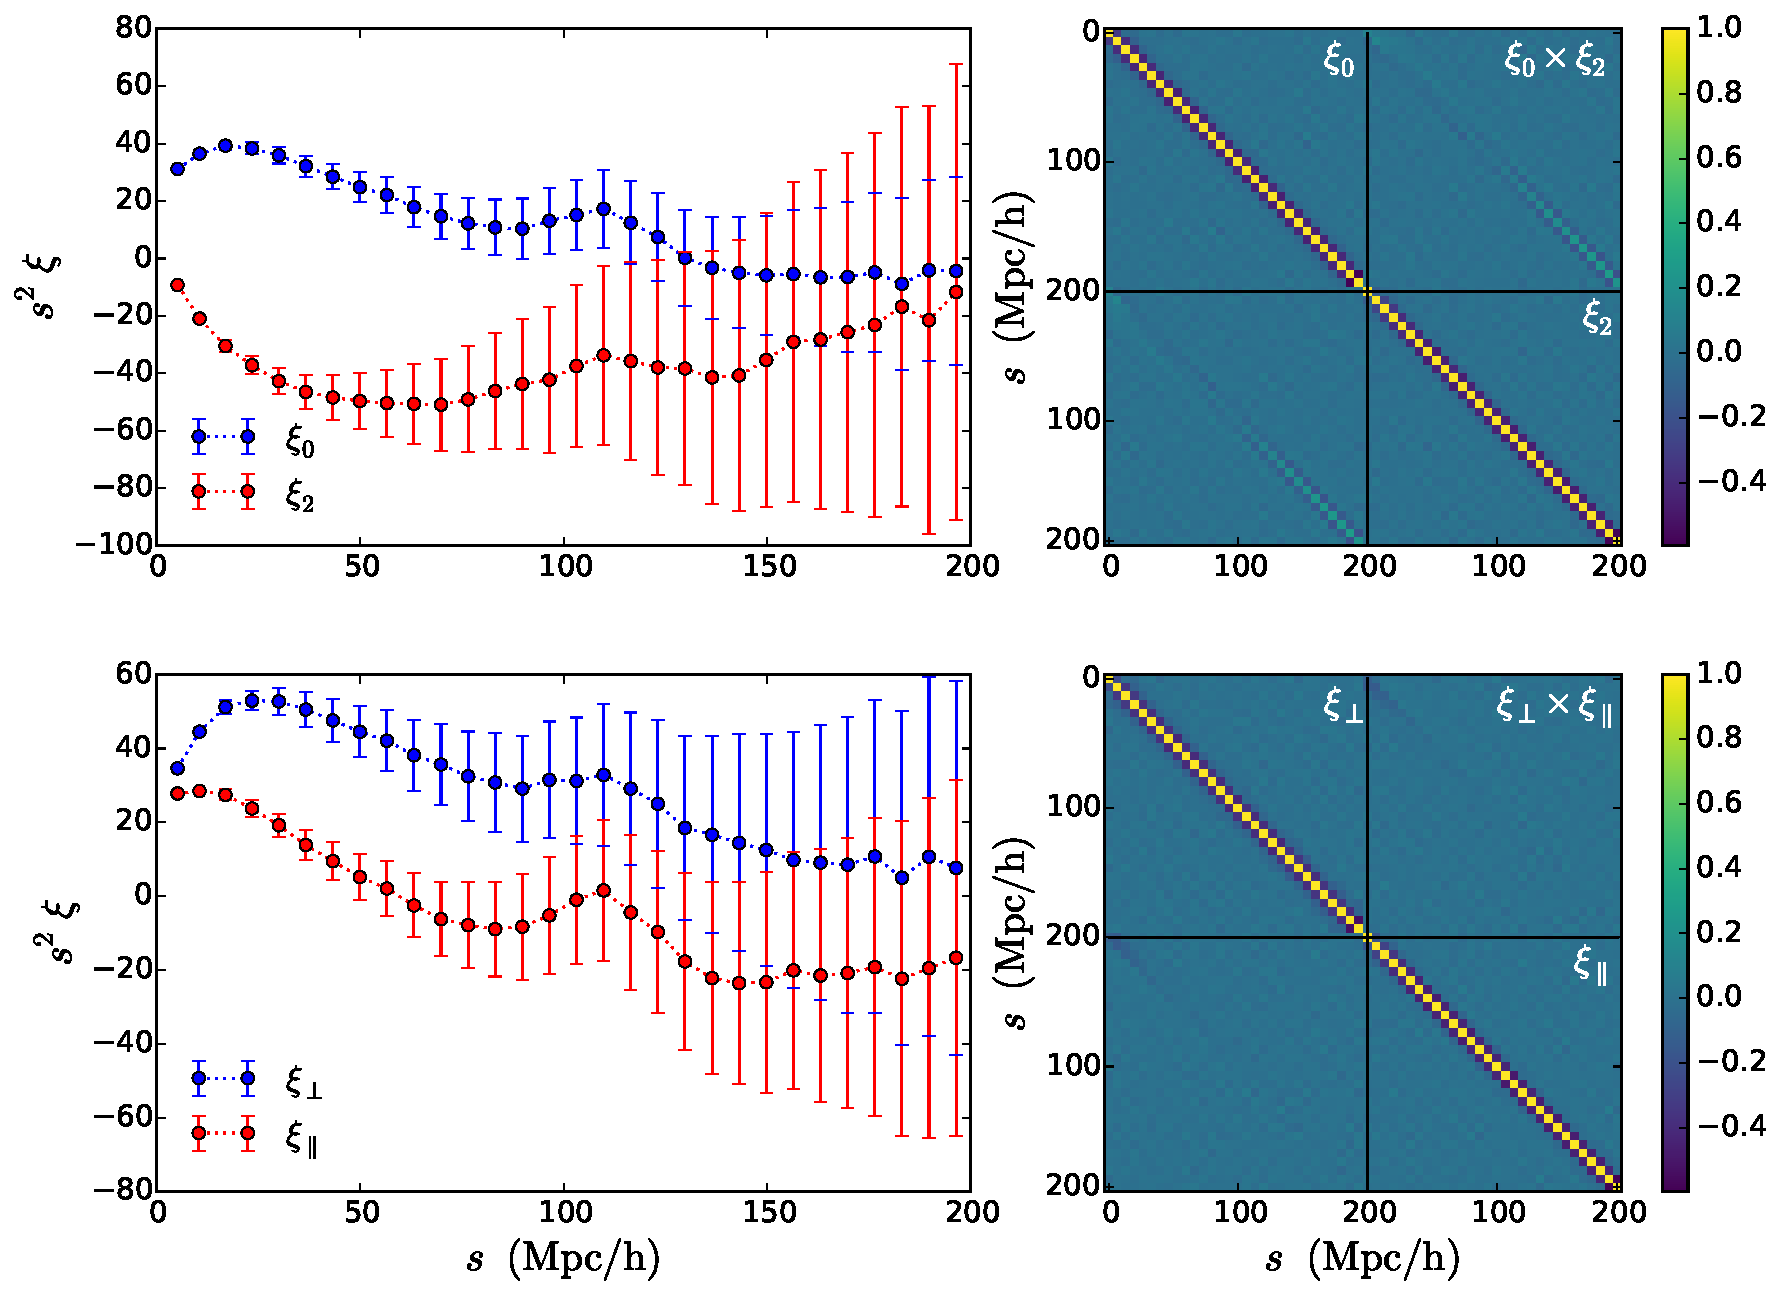
\includegraphics[width=0.95\textwidth]{images/wizcola.pdf}
	\end{center}
	\caption{The mean data points and covariance matrices for both the wedge and multipole expression of the WizCOLA data \citep{KazinKoda2014,KodaBlake2015}.  {\red **ADD A RECONSTRUCTED EXAMPLE FROM SIMS -- CHRIS TO FIND DATA.**}}
	\label{fig:wizcola}
	%\end{wrapfigure}
\end{figure*}


\section{The WiggleZ Dark Energy Survey}\label{sect:wigglez}

The WiggleZ Dark Energy Survey was carried out between 2006 to 2011 at the Australian Astronomical Observatory over the course of 276 nights \citep{Drinkwater2010}. The survey measured redshifts of $225\,415$ galaxy spectra, targeting blue emission-line galaxies in a redshift range of $0.2 < z < 1.0$. The target selection function is summarised in \citet{BlakeDavis2011}, and explained in detail in \citet{BlakeBrough2010}. 


A variety of analyses have already been conducted on the WiggleZ dataset. 
The one dimensional BAO signal was analysed for a subset of WiggleZ data in \citet{BlakeDavis2011}, and this analysis was refined by both including the full survey data and subdividing the data into redshift bins in \citet{BlakeKazin2011}. A final analysis of the 1D BAO signal involving reconstruction of the BAO peak was performed by \citet{KazinKoda2014}. 

Analyses of the 2D data have also been performed on WiggleZ data, but not yet on scales large enough to include the BAO peak.  \citet{BlakeBroughColless2011,ContrerasBlake2013} use redshift space distortions to measure the rate of growth  of structure, while \citet{BlakeGlazebrook2011} used the Alcock-Paczynski test on galaxy clustering as a {\em standard sphere} to measure expansion history. Cosmological results from the WiggleZ papers were combined with other surveys and datasets in \citet{Parkinson2012}. %For further publications using the WiggleZ dataset, see the publication list linked to from the WiggleZ home site.\footnote{\url{http://wigglez.swin.edu.au/site/}}\\

One investigation that has not been undertaken with the WiggleZ data is a two dimensional analysis of the BAO signal.  As the survey meets the criteria for being able to detect the 2D BAO signal -- volumes of order 1 Gpc$^3$ with order of $10^5$ redshifted galaxies \citep{Tegmark1997,BlakeGlazebrook2003,BlakeParkinson2006} -- we present that analysis in this paper.  

This analysis is motivated by two recent improvements to the WiggleZ survey data.  The first improvement is that reconstruction has now been performed to remove some of the effect of peculiar velocities \citep{KazinKoda2014}, which sharpens the BAO peak and thus makes it  easier to measure in the 2D correlation function (previous analyses had amplified the signal by averaging the information across all angles).  The second improvement is the creation of accurate mock catalogues from the WizCOLA simulations \citep{KodaBlake2015} for both the pre- and post-reconstruction data. The simulations provide more accurate covariance estimates than the lognormal realisations used in the early analyses.  We therefore also revisit the pre-reconstruction angle-averaged (1D) constraints from the final WiggleZ survey and present updated results.  By fitting our theoretical models to the mock data and recovering the correct cosmological model (the model that was used to make the simulations) we are able to perform rigorous checks that our correlation function models are sufficiently accurate, and optimise the range of scales over which the theory is adequate to include in the fits.  

Using simulations we found that the 2D information is best extracted from the full shape correlation function when it is decomposed into multipoles.  In contrast, after reconstruction the best way to extract the 2D information was by splitting the data into wedges along the line of sight and perpendicular to the line of sight.

Figure~\ref{fig:wizcola} shows the galaxy correlation function for a WiggleZ-like survey in three different forms.  The upper panel splits the 2D correlation function into the first two multipoles.  The middle and lower panels both show versions of the 2D correlation function split into wedges, which present the contributions from the modes parallel to the line of sight (red) and perpendicular to the line of sight (blue).  The middle panel shows the 2D correlation function as observed, whereas the lower panel shows the 2D correlation function after reconstruction has been applied.  You can see that reconstruction eliminates the shape difference between the wedges and strengthens the BAO peak. 

%Whilst this may not give tight cosmological constraints due to the number of galaxies being only barely above the minimum needed to detect the 2D BAO peak, the results obtained will be largely independent of priors from CMB based surveys such as Planck or WMAP and can be combined with other survey results.





\section{The 2D Correlation Function}
\label{sec:model}

\subsection{Base Model --- before reconstruction}
For fits to the unreconstructed data, we fit against not just the BAO peak, but also to the broad shape of the correlation function. We begin the model with a linear power spectrum $P_{\rm{lin}}(k)$, which is  generated using the \camb{} software created by \citet{Lewis2000}. We limit our analysis to a Flat $\Lambda$CDM cosmology, appropriate as the data are of insufficient strength to tightly constrain more parameters.
We set $\Omega_c h^2$ as a free parameter, and fix other values to the WizCOLA simulation fiducial cosmology in our analysis, such that $\sigma_8 = 0.812$, $n_s=0.961$, $h = 0.705$. We fix $\Omega_b h^2$ to $0.0226$, as $\Omega_b h^2$ is well constrained by CMB data and variations even up to $5\sigma$ are negligible to the BAO model when testing Flat $\Lambda$CDM cosmology. This value is consistent with the WizCOLA simulation value $\Omega_b h^2 = 0.02266$. 

We model the BAO peak smoothing caused by displacement of matter due to bulk flows with a smoothing parameter \citep{CrocceScoccimarro2008, SanchezBaughAngulo2008, Sanchez2009, BlakeDavis2011, BeutlerBlake2011}. This smoothing parameter takes the form of a Gaussian dampening term which reduces the amplitude of the BAO signal as a function of $k$:
\begin{align} \label{{eq:blake1}}
	P_{\rm{dw}}(k) = e^{-k^2 \sigma_v^2} P_{\rm{lin}}(k) + (1 - e^{-k^2 \sigma_v^2}) P_{\rm{nw}}(k),
\end{align}
where $P_{\rm{nw}}(k)$ is a power spectrum without the BAO signal. Whilst advances in renormalization perturbation theory  \citep[RPT;][]{CrocceScoccimarro2008} allow a theoretical determination of $\sigma_v$ as
\begin{align} \label{eq:sigmav}
\sigma_v^2 = \frac{1}{6\pi^2} \int P_{\rm{lin}}(k)\, dk,
\end{align}
however $\sigma_v$ is set to a free parameter due to inaccuracies in the theoretical determination from non-linear effects.

In most studies the power spectrum without the BAO signal present is generated using the \verb;tffit; algorithm given by \citet{EisensteinHu1998}. \citet{ReidPercival2010} investigated an alternate method of generating a no-wiggle power spectrum from the linear \camb{} power spectrum in which an 8 node b-spline was fitted to the linear power spectrum, concluding the likelihood surfaces generated when fitting using splines and the algorithm from \citet{EisensteinHu1998} agree well. For our work we introduce a new method to attain a no-wiggle power spectrum $P_{\mathrm{nw}}(k)$ utilising polynomial subtraction. For a comparison of this methodology against the \verb;tffit; algorithm supplied by \citet{EisensteinHu1998} or spline fitting, please see Appendix \ref{app:dewiggle}.


The non-linear effects of gravitational growth are incorporated by using \halofit{} from \citet{Smith2003}, %as used by \citep{ReidPercival2010, BlakeDavis2011, ChuangWang2012} 
which generates a power ratio $r_{\rm{halo}}$ as a function of $k$ 
\begin{align}
	P_{\text{nl}} = P_{\text{dw}} r_{\text{halo}}.
\end{align}
We take into account galaxy bias $b$ by $\xi_{\rm galaxy}(s) = b^2 \xi(s)$ and we follow \citet{BlakeDavis2011} who incorporate scale dependent bias derived from the Gigglez simulations, $B(s)$, into to the model, via
\begin{align}
	\xi_{\rm{galaxy}}(s) = B(s) \xi(s),
\end{align}
where $B(s) = 1 + (s/s_0)^\gamma$, with $s_0 = 0.32 h^{-1}\,$Mpc and $\gamma = -1.36$.




The Kaiser effect from coherent infall can be modelled simply in Fourier space \citep{Kaiser1987}:
\begin{align} \label{eq:gaztanga1}
	P_{\rm{nl}}(k, \mu) = (1 + \beta \mu^2)^2 P_{g}(k),
\end{align}
where $P_{g}$ is the power spectrum of galaxy density fluctuations $\delta_g$, $\mu$ is the cosine of the angle to line of sight, and $\beta = f/b$ and $f$ is the growth rate of growing modes in linear theory. %This correction for the Kaiser effect has been utilised by \citet{Gaztanaga2009, ChuangWang2012, XuPadmanabhan2012} for identifying the unreconstructed BAO signal in survey data. 
When reconstructing the BAO signal \citep[see][for details]{PadmanabhanXuEisenstein2012,KazinKoda2014}, the Kaiser effect is corrected for and thus does not have to be inserted into the cosmological model.

Peculiar velocity does not have to be coherent to effect observational cosmology, and the random peculiar velocities of galaxies in clusters, which are related to the cluster mass via the virial theorem, create artifacts known as Fingers of God. In the investigation of growth rate with WiggleZ data, \citet{BlakeBroughColless2011} adopts a Lorentzian model of velocity dispersion with
\begin{align}
	P_{\rm{gal}} = \frac{1}{1 + (k \sigma_V \mu)^2}  P_{\rm{nl}}(k, \mu), \label{eq:lorentzian}
\end{align}
where $\sigma_V$ is the pairwise peculiar velocity dispersion. We adopt this in our analysis. For a more complete treatment of the underlying model, see \citet{HintonThesis2015}.









\subsubsection{Moving to a correlation function} \label{sec:prior:cor}

The power spectrum and correlation functions are related to each other via Fourier transform. One dimensional BAO analyses generally look at the angle-averaged correlation function, which is simply the monopole moment. A power function can be decomposed into its multipole components via 
\begin{align}
	P_{\ell}(k) = \frac{2\ell + 1}{2} \int_{-1}^1 P_{\rm{gal}}(k, \mu) \ \mathcal{L}_\ell \  d\mu
\end{align}
where $\mathcal{L}_\ell$ represents the $\ell$'th Legendre polynomial. These multipole components can be turned into correlation functions by Fourier transforming them, giving
\begin{align}
	\xi_\ell(s) = \frac{1}{(2\pi)^3} \int 4\pi k^2 \ P_\ell(k) \ j_\ell(ks)
\end{align}
where $j_\ell(ks)$ are spherical Bessel functions of the first kind. The increased power of small scale oscillations from the non-linear corrections decreases convergence of this function, so we multiply the integrand by a Gaussian factor $\exp(-k^2 a^2)$ to improve convergence, where we found $a=0.5 h^{-1} \rm{Mpc}$ to be the optimal factor to improve computational speed while maintaining accuracy \citep{HintonThesis2015}.  \citep[The results are not sensitive to the exact choice of $a$;][set $a= 1\, h^{-1}\rm{Mpc}$]{AndersonAubourg2012}. %This is in contrast to other methods that may be used to increase convergence, such as truncating the numerical integral after a specific number of periods in the spherical Bessel function. Whilst the \citet{BlakeDavis2011} WiggleZ analysis does not contain the Gaussian dampening term seen in \citet{AndersonAubourg2012}, it is introduced in the correlation function model used in \citet{BlakeKazin2011}. We performed an investigation of numerical deviations from the true correlation function using an unmodified equation, truncation, and a Gaussian dampening term, and these can be found in Appendix \ref{app:pk2xi}.  Based on these results we introduce a Gaussian dampening factor of  $a= 0.5\, h/\rm{Mpc}$.



\subsubsection{Multipoles and Wedges}

It is impractical to fit the data to a full 2D correlation function, as the calculation of the covariance matrix is infeasible.  Instead one typically reduces the 2D information into a simplified measure that encapsulates the essential anisotropy.  Two methods by which this can be done are wedges and multipoles.  

The wedges method splits the 2D correlation function into wedges based on angle, and averages the correlation function in that wedge.  The multipole method decomposes the correlation function into multipoles.  For extended treatment of the mathematics, see \citet{KazinSanchezBlanton2012, KazinSanchezCuesta2013, SanchezKazinBeutler2013, XuCuesta2013}. 

In all cases we have used a fiducial cosmology to convert observed right ascension, declination, and redshift into distances (separations) and thus generate the correlation function.  So the variables we fit for are not the distances (separations) themselves, but rather the ratio of the distance in the true model to the distance in the fiducial model.  This is achieved by scaling the model distances to give $s_{\rm test}= \alpha s_{\rm model}$.   

	Thus the primary variable we fit for is $\alpha$.  Depending on which type of analysis we are performing, $\alpha$ relates to  distances in different ways.  \citet{BlakeDavis2011} show, for example, the degeneracy lines between $\alpha$ and $\Omega_{\rm M}$ and how they change depending on whether you fit to the correlation function shape, the BAO peak only, or the power spectrum.  When fitting to the BAO peak, the degeneracy direction lies along a line of constant $r_s/D_V$ (in the 1D case) where $D_V=***$ and  $r_s$ is the sound horizon at drag epoch, given by
	\begin{align}
	r_s = \frac{c}{\sqrt{3}} \int_0^{1/(1+z)} \frac{da}{a^2 H(a) \sqrt{1 + (3\Omega_b/4\Omega_\gamma) a}}, \label{eq:rs}
	\end{align}
	with $\Omega_\gamma = 2.469\times10^{-5} h^{-2}$ for $T_{{\rm cmb}}=2.725$ and $\Omega_r = \Omega_\gamma(1 + 0.2271 N_{{\rm eff}})$, where we utilise $N_{\rm eff} = 3.04$.
	However, when fitting for the correlation function shape the degeneracy direction lies along a line of constant $A=D_V(z) \sqrt{\Omega_m H_0^2} / zc$, which was a parameter introduced by \citet{Eisenstein2005} for exactly that reason.  Note that $A(z)$ does not depend on $r_s$.  


When we update the pre-reconstructed angle averaged 1D measurement of \citet{BlakeKazin2011} we fit for 
\begin{align}
\alpha = \frac{D_V(z)}{D_V^{\prime}(z) }.\label{eq:DvDv}
\end{align}

For the multipole expansion used in the 2D pre-construction fits, we fit a scaling factor $\alpha$ and warping parameter $\epsilon$ such that
\begin{align}
\alpha(1 + \epsilon)^2 \approx \alpha(1 + 2\epsilon) &\approx \frac{H^\prime(z)}{H(z)} \label{eq:alpha1}\\
\alpha(1 + \epsilon)^{-1} \approx \alpha(1 - \epsilon) &\approx \frac{D_A(z)}{D_A^\prime(z) }. \label{eq:alpha2}
\end{align}





%We thus now have two complete models for generating theoretical correlation functions both in wedge and multipole format. %The final concern that needs to be addressed is what data range should be fit on, the optimal range of data to fit is dependent on the data set used and the accuracy of the models.  %which is unfortunately a source of great variability in prior literature.




%\subsection{Final Model}

%Having determined fitting ranges and created a theoretical model piece by piece, we can now summarise. 
In summary, our model generates a linear power spectrum, with input parameter $\Omega_c h^2$. The dampening term $k_*$ (equivalently $\sigma_v$), galaxy bias $b^2$, growth rate $\beta$, and Lorentzian factor $\sigma_V$ are marginalised over, leaving final constraints in the form of $\Omega_c h^2$, $\alpha$ and $\epsilon$. %Transformation parameters $\alpha$ and $\epsilon$ are used for the multipole data expression that we use for unreconstructed data, and $\alpha_\parallel$ and $\alpha_\perp$ are used for the wedge analysis that we use for the reconstructed data.  Thus when we perform the final fit the set of parameters we vary are $\Omega_c h^2$, $k_*$, $\sigma_V H$, $\beta$, $b^2$ and transformation parameters. We marginalise over all but $\Omega_c h^2$, $\alpha$, \& $\epsilon$ for multipole expansion.



\subsection{Base model --- after reconstruction}

\citet{EisensteinSeoSirko2007} proposed that the ``blurring'' of the baryon
acoustic peak due to the large-scale coherent motion of galaxies could
be partially remedied by a procedure of ``linear reconstruction,'' in
which the displacement field $\vec{\psi}$ is estimated from the
observed density field using linear theory, and used to retract
galaxies by $-\vec{\psi}$ to an approximation of their initial
position.  In \citet{KazinKoda2014} we applied density-field
reconstruction to the WiggleZ Survey data, and demonstrated that it
resulted in a sharpening of the acoustic peak in the angle-averaged
correlation function and thereby in improved distance constraints,
with consistent behaviour found in mock catalogues.  We overcame edge
effects and holes within the survey by applying a Weiner-filtering
procedure similar to that presented in \citet{PadmanabhanXuEisenstein2012}.  For
full details of the procedure please refer to \S 2.3 in
\cite{KazinKoda2014}.

We now examine the anisotropic baryon acoustic peak signature present
in the reconstructed WiggleZ density field, marginalizing over the
broadband shape information.  A full description of our procedure is
given in our previous analysis of the SDSS DR9 CMASS galaxies
\citet[][see \S 5.3]{KazinSanchezCuesta2013}.  In brief, we measured the
correlation function of the reconstructed data in two ``clustering
wedges''.  One could in principle have many wedges, but for our data (and all previous data) the signal to noise limits us to two wedges -- one taking the half of the data along the line of sight ($\mu\ge0.5$), the other perpendicular to it ($\mu<0.5$), where $\mu$ is the cosine of the angle with respect to the line of sight.
We fitted the data assuming a BAO template including
quasi-linear corrections based on the renormalized perturbation theory
of \citet{CrocceScoccimarro2008}. This template is distorted in the tangential
and radial directions by parameters $\alpha_\perp$ and
$\alpha_\parallel$ which are given by
\begin{align}
\alpha_\perp &\approx \frac{D_A(z) r^\prime_s }{D_A^{\prime}(z) r_s}, \label{eq:alphaperp}\\
\alpha_\parallel &\approx \frac{H^{\prime}(z) r^\prime_s}{H(z) r_s},\label{eq:alphaparallel}
\end{align}
where the $r_s$ term can be found (unlike in the pre-reconstruction $\alpha$) due to the degeneracy direction of fitting only for the BAO peak.

  


We assume a flat prior in $(\alpha_\perp,\alpha_\parallel)$ between
0.5 and 1.5.  For each clustering wedge we also marginalized over an
amplitude parameter and the coefficients of three additive polynomial
terms, producing a 10-parameter model.  We explore the parameter space
using MCMC chains, and present results for
$(\alpha_\perp,\alpha_\parallel)$, marginalizing over the other 8
parameters.


\section{Validation of unreconstructed multipole analysis}
\label{sec:test}

To validate our model we employ several tests.  Firstly we compare it to past analyses (the 1D WiggleZ results) and then in more detail to simulated data (WizCOLA).  Following that we test two methods by which to combine the information in the different redshift bins.


\begin{comment}

\subsection{Choice of statistical measures}
An often-overlooked aspect of comparing constraints is that the choice of statistics used to extract parameter bounds -- the process of moving from likelihood surface to specifying numeric constraints -- can have a noticeable affect on the final constraints reported. In this analysis we report maximum likelihood statistics, where we give the point of maximum likelihood and asymmetric errors. This is in contrast to the results of the WiggleZ 1D BAO analysis presented in \citet{BlakeDavis2011}, which utilised mean statistics.


\end{comment}



%Having generated a model correlation function, the final step is to compare that against the correlation function computed with observational data and a fiducial cosmology. However, as the created model breaks down at low distances and all models are similar at high distances where sample variance increases data uncertainty, matching normally only occurs on a subsection of the data. Comparisons between different papers are shown in Table \ref{tab:truncation}. Given the wide range of dataset truncation values and lack of clear support for one cutoff over another, this represents a parameter that requires investigation. This investigation can be found in Appendix \ref{app:truncation}, and we conclude that a data range of $25 < s < 180 h^{-1} \ \rm{Mpc}$ allows maximum utilisation of available data without introducing bias into our model.








\subsection{Validation against prior WiggleZ analyses}


We use our model to repeat the 1D BAO analysis using the WiggleZ unreconstructed dataset over the same data range utilised by \citet{BlakeDavis2011} and \citet{BlakeKazin2011}: $10<s<180 h^{-1}\rm{Mpc}$. Our model is very similar to the one used by \citet{BlakeKazin2011}, but differs from theirs by implementation (MCMC methods in comparison to a grid search), dewiggling methodology, covariance matrix, and choice of statistical measures reported \citep[we use maximum likelihood statistics, as opposed to mean statistics used in][]{BlakeDavis2011}. The most important difference in the analysis is that we use the improved knowledge of covariances from the WizCOLA simulations \citep[as compared to the lognormal realisations used in][]{BlakeKazin2011}.

We first fit using $\sigma_v$ as a free parameter, and finding $\sigma_v$ unconstrained, fix it to a specific value. We fix $\sigma_v = 5 h^{-1}$ Mpc, which is approximately its theoretically expected value.  This gives tighter constraints due to the fewer degrees of freedom, and does not bias results since the fit is insensitive to the value of this parameter (mean parameter deviation between fixing $\sigma_v$ and fitting for $\sigma_v$ was less than $0.05\sigma$). The likelihood surface for our fits can be seen in Figure \ref{fig:fmonopole}, and our results are compared in Table \ref{tab:blakekazintable}. 


\begin{figure}
	\begin{center}
		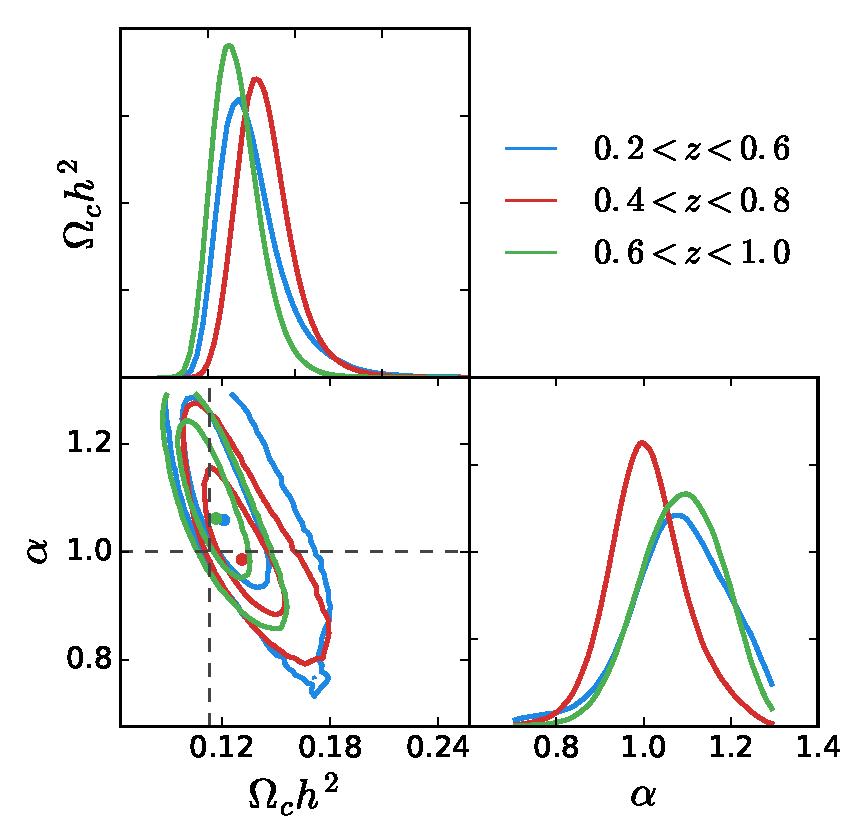
\includegraphics[width=\columnwidth]{images/fMonpole.pdf}
	\end{center}
	\caption{Likelihood surfaces when fitting the 1D BAO signal from WiggleZ using the new WizCOLA covariance matrices. Parameters $b^2$, $\beta$, and $\sigma_V$ are marginalised over, with $\sigma_v$ set to $5 h^{-1}$ Mpc.}
	\label{fig:fmonopole}
\end{figure}



\begin{table*}
	\centering
	\caption{A comparison between the fits found in this analysis and those found in \citet{BlakeKazin2011}. These analyse the same data, but this analysis uses a slightly different model and an improved covariance matrix. The results given in \citet{BlakeKazin2011} use mean statistics, whilst we utilise maximum likelihood statistics, but the dominant difference comes from the improved covariance matrix. }
	\begin{tabular}{cc|ccc|ccc}
		\specialrule{.1em}{.05em}{.05em} 
		Sample & $z_{\rm{eff}}$ & \multicolumn{3}{c}{\citet{BlakeKazin2011}}  & \multicolumn{3}{c}{This analysis}\\
		&  & $\chi^2{\rm DoF}$ & $\Omega_m h^2$ &$\alpha$ & $\chi^2/{\rm DoF}$ & $\Omega_m h^2$ & $\alpha$ \\
		\specialrule{.1em}{.05em}{.05em} 
		$0.2 < z < 0.6$ & $0.44$ & $0.88$ & $0.143\pm0.020$ &$1.024\pm0.093$ & $1.01$ & $0.143\pm 0.017$ & $1.07^{+0.13}_{-0.09}$ \\
		$0.4 < z < 0.8$ & $0.60$ & $0.78$ & $0.147\pm0.016$ &$1.003\pm0.065$ & $0.85$ & $0.151^{+0.017}_{-0.014}$ & $1.00^{+0.09}_{-0.08}$ \\
		$0.6 < z < 1.0$ & $0.73$ & $1.05$ & $0.120\pm0.013$ &$1.113\pm0.071$ & $1.22$ & $0.138^{+0.012}_{-0.015}$ & $1.10^{+0.09}_{-0.10}$ \\
		\specialrule{.1em}{.05em}{.05em} 
	\end{tabular} \label{tab:blakekazintable}
\end{table*}
\begin{comment}
BlakeKazin2011 uses larger data pins. 17 bins, 4 parameters, 13DoF, which is why there was a difference. I have 29DoF.
\end{comment}


We see that most results follow closely those obtained in \citet{BlakeKazin2011}, however the result of $\Omega_m h^2 (z_{\rm eff} = 0.73)$ shifts by more than $1\sigma$. This shift increases the value of $\Omega_m h^2 (z_{\rm eff} = 0.73)$, bringing it into agreement with the $\Omega_m h^2$ determination from the other redshift bins. These shifts were confirmed to be due to the change in covariance matrix and not any difference in changes to the modeling process, as rerunning the same fit using the original lognormal realisations bought the deviation to below $0.5\sigma$. %Swapping parameter statistics from maximum likelihood to mean statistics did not significantly improve agreement. 
 Comparison against fits using the WizCOLA covariance and lognormal covariance indicate in all redshift bins that the dominating contribution in fit difference is due to the improved covariance. As our analysis shows no signs of significant bias or difference due to modelling when compared against \citet{BlakeKazin2011}, we proceed to the 2D BAO model.






\subsection{Fitting range} \label{sec:trunc}
Before fitting our model correlation function to the data, we need to assess the range of scales over which the data are useful.  We expect the model to do poorly at small distances (where non-linearities are strong), while the data's sample variance increases at large distances.  So there will be an optimal range of scales over which to fit the data, and that range will be dependent on the data set (less biased tracers can go to smaller scales, larger volume data sets can go to larger scales).  We determined our optimal fitting range using simulations \citep[see][]{HintonThesis2015}  and conclude that a data range of $25 < s < 180 \hMpc$ allows maximum utilisation of available data without introducing bias into our model. 
{\red **[SAM. Sample variance does increase, and I go over that in my thesis but its not covered here for brevit. Unsure how to address this comment] Chris said referee will argue the the sample variance increasing at large distance -- why?**}




\subsection{Validating the multipole expansion model against WizCOLA data}

 To validate our model we test it against the WizCOLA simulations.  WizCOLA used known survey geometry and an underlying fiducial cosmology to simulate 600 realisations of the WiggleZ survey, where the fiducial cosmology is parameterised by $\Omega_m = 0.273$, $\Omega_\Lambda = 0.727$, $\Omega_b = 0.0456$, $h=0.705$, $\sigma_8 = 0.812$ and $n_s = 0.961$ following WMAP cosmology \citep{Komatsu2009}.  Putting this in terms of $\Omega_c h^2$, we have $\Omega_c h^2 = 0.113$. We fit against these individual realisations and compare the distribution of our recovered results to the known fiducial cosmology, and also fit to the mean of all 600 simulations to create a single high quality dataset, where the variance of the data was reduced by a factor of $\sqrt{600}$ as the simulations are independent. 

%\subsubsection{Validating the multipole expansion model}


%In this section we validate the mutipole expansion representation of our model using the WizCOLA simulations. 


As the cosmology used in the WizCOLA simulations is identical to the fiducial cosmology values used to extract data from the WizCOLA simulations, we do not expect to observe anisotropic warping when fitting to the simulation realisations.   As such, we can validate our model by ensuring that it recovers $\alpha = 1.0$ and $\epsilon = 0.0$ when fitting the WizCOLA correlation functions.

  Prior analyses have found poorly constrained values for $k_*$ \citep{BlakeDavis2011} using Wigglez data, and to validate that the bounds applied to $k_*$ in prior analyses were not influencing or biasing fits, we take the mean realisation dataset (with its increase data strength) and instead fit to $\log(k_*)$, allowing us to check if $k_*$, when unconstrained over order-of-magnitude, provides a best fit value within the bounds imposed in prior results. Final parameter constraints are detailed in Table \ref{tab:wizmp}.

For all redshift bins, our best fits recovered the fiducial parameters well within the $1\sigma$ uncertainty limit. We can also see that, looking at the mean value of the determined values for $\log(k_*) = -2.10$, this gives a $\sigma_v = 5.77 h^{-1}$ Mpc, which is in the magnitude expected by the theory given in equation \eqref{eq:sigmav} and the values found found in \citet{BlakeKazin2011} and \citet{BlakeDavis2011}.
Within the range $\sigma_v \in [0,10]$, we find no significant difference in $\chi^2$ values, indicating that $\sigma_v$ is not tightly constrained within theoretically predicted ranges. Fixing $\sigma_v = 5 h^{-1}$ Mpc, has negligible effect on the cosmological parameters of interest, and therefore we do that for the rest of our analysis.

\begin{table*}
	\centering
	\caption{Recovered parameter constraints when fitting to the combined 600 realisations of the WizCOLA simulation data multipoles.}
	\begin{tabular}{cc|ccccc}
		\specialrule{.1em}{.05em}{.05em} 
		Sample & $z_{\rm{eff}}$ & min $\chi^2$ & $\Omega_c h^2$ &$\alpha$ & $\epsilon$ & $\log(k_*)$\\
		\specialrule{.1em}{.05em}{.05em} 
		$0.2 < z < 0.6$ & $0.44$ & $12.0$ & $0.112^{+0.005}_{-0.006}$ &$1.006^{+0.023}_{-0.022}$ & $0.002^{+0.016}_{-0.016}$ & $-2.18^{+0.22}_{-0.20}$\\
		$0.4 < z < 0.8$ & $0.60$ & $8.6$  & $0.114^{+0.005}_{-0.004}$ &$1.004^{+0.017}_{-0.016}$ & $0.005^{+0.012}_{-0.010}$ & $-2.05^{+0.20}_{-0.17}$\\
		$0.6 < z < 1.0$ & $0.73$ & $10.8$ & $0.113^{+0.005}_{-0.005}$ &$1.006^{+0.021}_{-0.018}$ & $0.007^{+0.015}_{-0.012}$ & $-2.07^{+0.26}_{-0.23}$\\
		\specialrule{.1em}{.05em}{.05em} 
		Input & & & 0.113 & 1.0 & 0.0 & \\
		\specialrule{.1em}{.05em}{.05em} 
	\end{tabular}\label{tab:wizmp}
\end{table*}


\begin{comment}
\begin{figure}
	%\begin{wrapfigure}{r}{0.5\textwidth}
	\begin{center}
		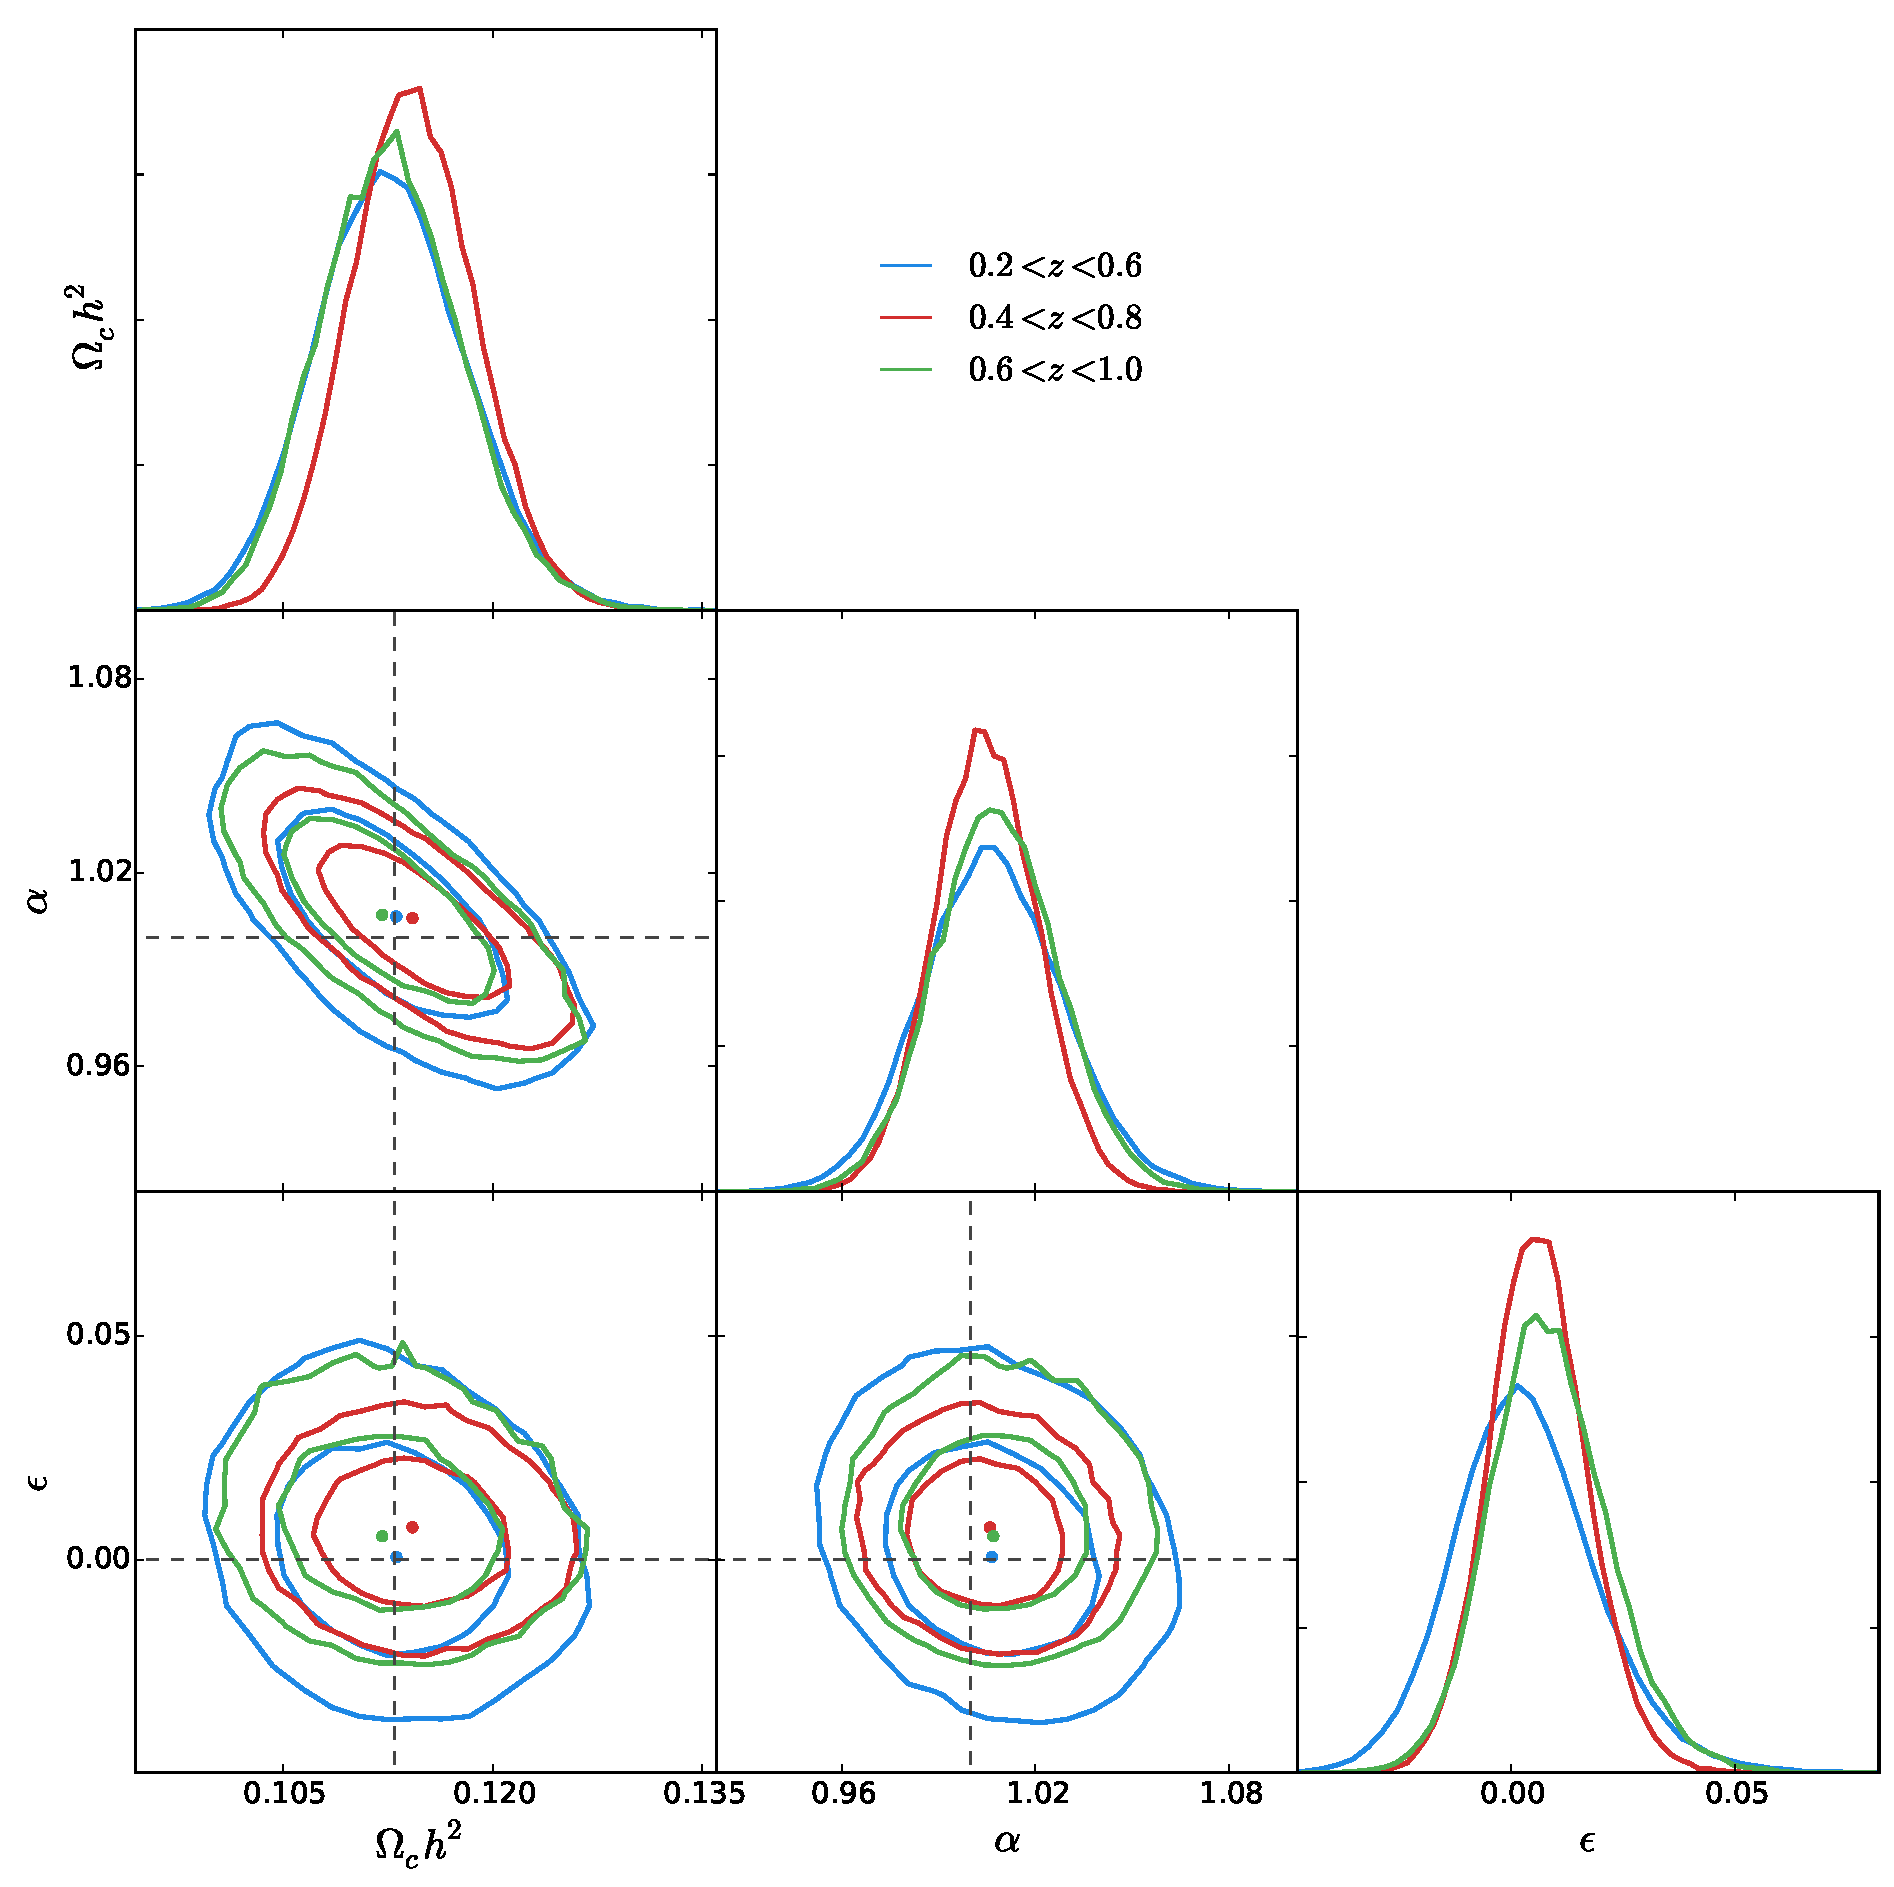
\includegraphics[width=\columnwidth]{images/wizmp.pdf}
	\end{center}
	\caption{Model fits using the mean data from the 600 WizCOLA realisations, where we are fitting to the multipole expansion. The dashed line represents the fiducial parameters of $\Omega_c h^2 = 0.113$, $\alpha=1.0$, $\epsilon=0.0$. }
	\label{fig:wizmp}
	%\end{wrapfigure}
\end{figure}
\end{comment}

Some past surveys have included hexadecapole terms in the multipole analysis \citep{XuCuesta2013}. In order to test the significance of the hexadecapole term, we ran the above analysis with and without it. We find that the statistical uncertainty dominates any loss of information contained in the hexadecapole signal. Due to computational constraints and the low impact of the term, the hexadecapole contribution was left out of the final model.

% The comparison likelihood surfaces are shown in Figure \ref{fig:wizmpfastComp}, and 
\begin{comment}
\begin{figure}
	%\begin{wrapfigure}{r}{0.5\textwidth}
	\begin{center}
		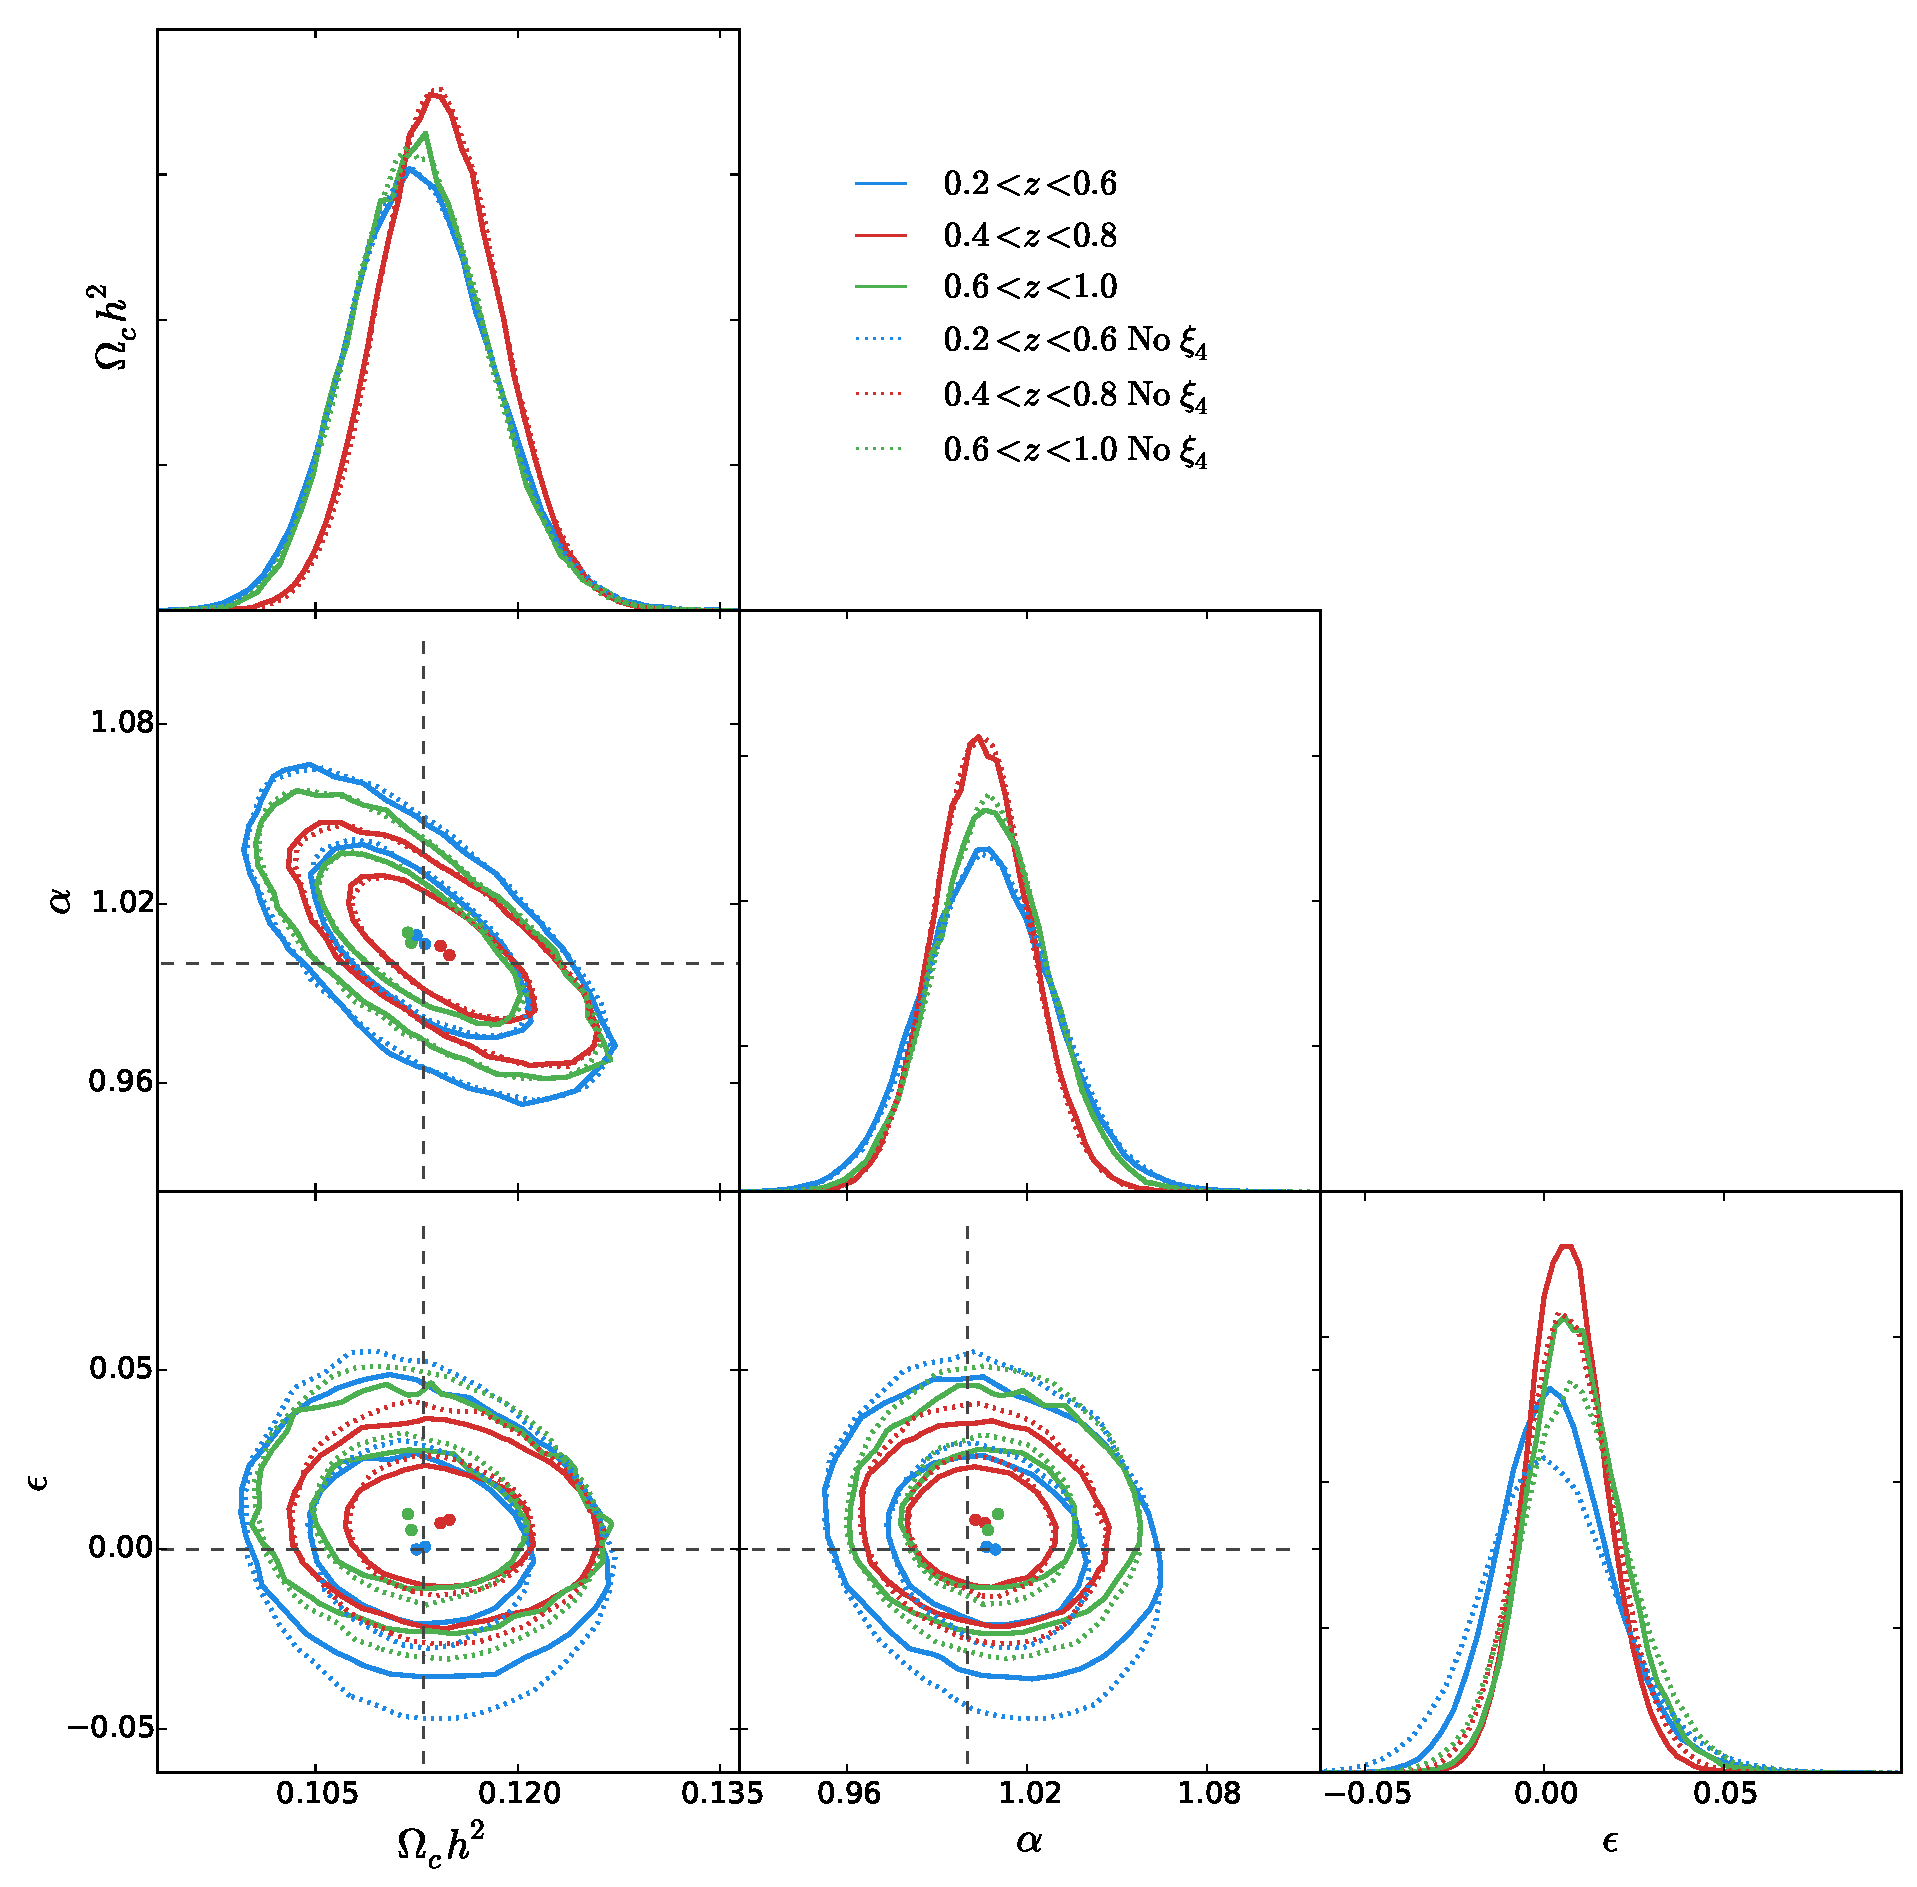
\includegraphics[width=\columnwidth]{images/wizmpfastComp.pdf}
	\end{center}
	\caption{A comparison of likelihood surfaces for the WizCOLA data when including the contribution from the hexadecapole term and when discarding it. Any change in likelihood surfaces and final distributions is negligible when compared to the statistical uncertainty in the final results.}
	\label{fig:wizmpfastComp}
	%\end{wrapfigure}
\end{figure}
\end{comment}

Finally, we can perform a final validation of the multipole methodology by fitting to individual realisations of the WizCOLA simulation instead of the mean data set. %Due to the decreased data strength, we move from allowing the parameter $\log(k_*)$ to vary, to fixing the parameter $\sigma_v = 5\,$h$^{-1}$ Mpc, which was validated using the mean simulation data. Fixing the parameter was not found to significantly modify output parameters, and a reduction in the number of free parameters results in tighter constraints, in addition to faster MCMC chain convergence. 
The results are shown in Figure \ref{fig:mpDist2}, which confirms that the recovered parameter distribution matches the simulation.  

For small $\epsilon$, cosmological parameters can be extracted via Eq.~\ref{eq:alpha1} and Eq.~\ref{eq:alpha2}.  {\red [SAM: Not sure what to put here.  Thoughts?] The degeneracy direction of $\alpha$---$\Omega_c h^2$ lies along a line of constant (**?**), which justifies our use of $\alpha=(1+\epsilon)^2\approx H^\prime(z)/H(z)$. ***ELABORATE*** }


\begin{figure}[h!]
	%\begin{wrapfigure}{r}{0.5\textwidth}
	\begin{center}
		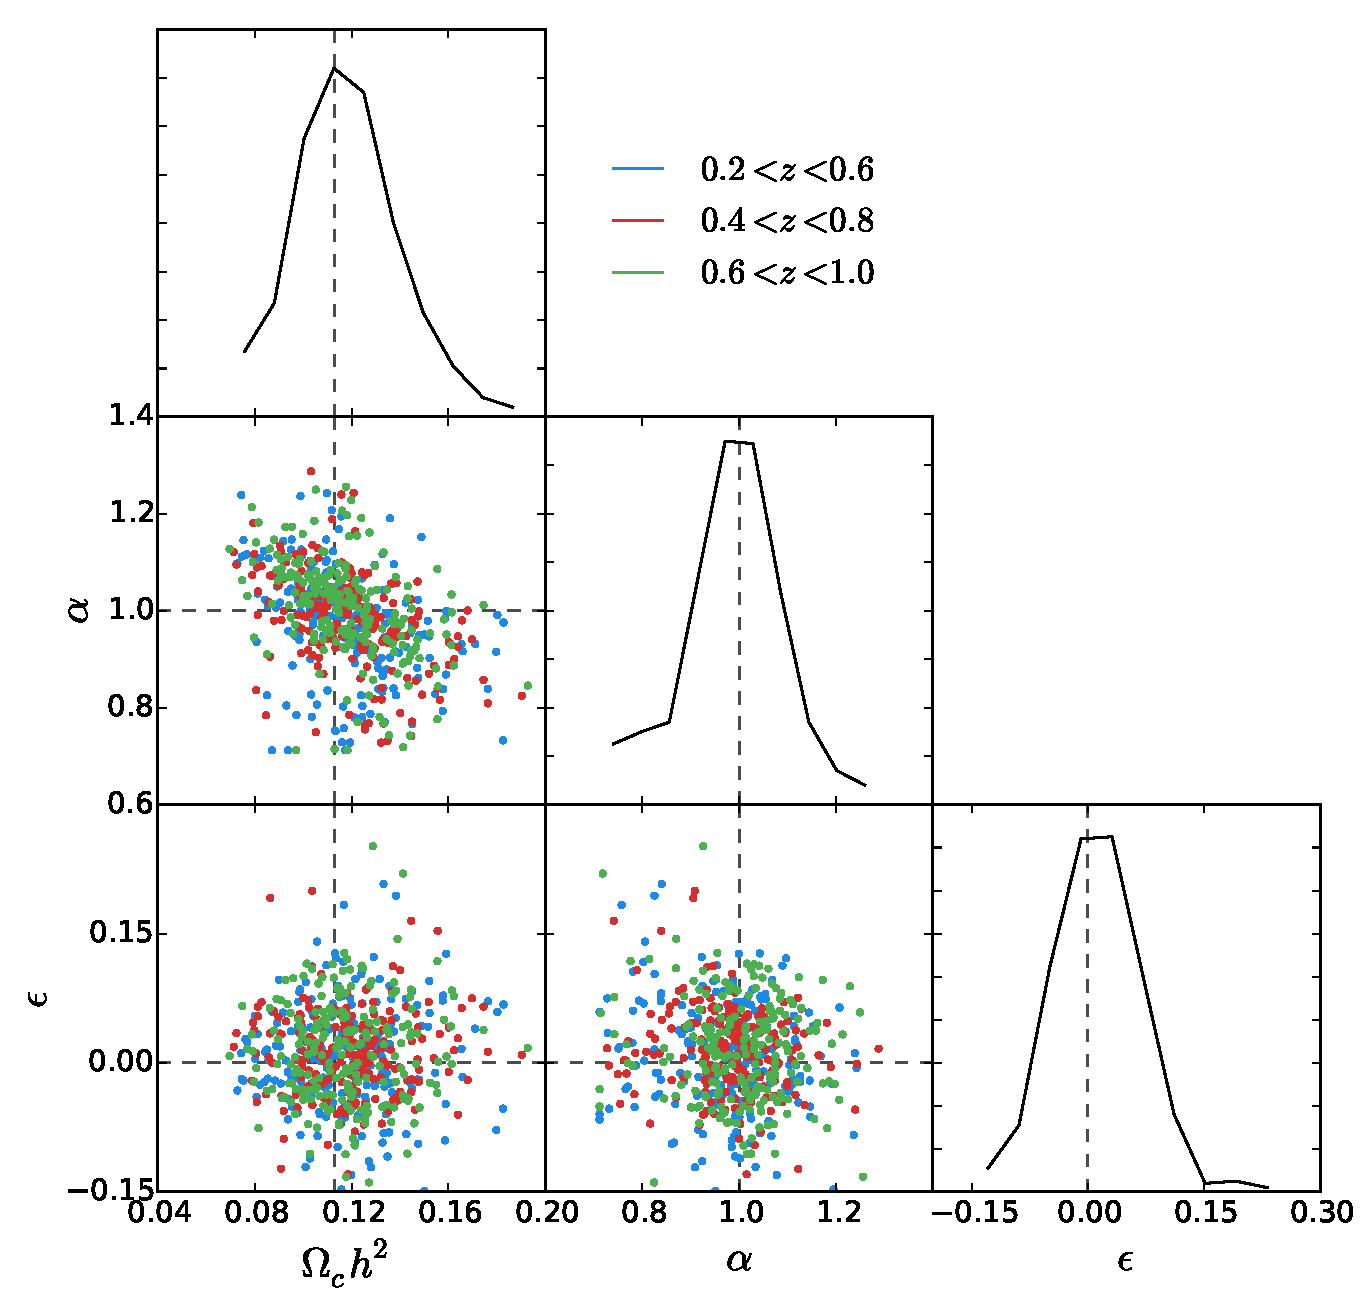
\includegraphics[width=\columnwidth]{images/mpDist2.pdf}
	\end{center}
	\caption{Maximum likelihood $\Omega_c h^2$, $\alpha$ and $\epsilon$ values from WizCOLA realisations of the WiggleZ data are shown in the bottom left corner plots. Dashed black lines indicate simulations parameters, and the solid black distributions in the diagonal subplots represent the final distribution across all bins for the specific parameter. {\blue A pre-reconstruction wedge analysis was not performed due to unconstrained parameter distributions, see \citet[\S 4.3]{HintonThesis2015} for more details.}}
	\label{fig:mpDist2}
	%\end{wrapfigure}
\end{figure}



\subsection{Combining redshift bins for multipole data}

The data present in the WizCOLA simulations and the final WiggleZ dataset is available in three redshift bins, $0.2 < z < 0.6$, $0.4 < z < 0.8$, and $0.6 < z < 1.0$. If these bins were independent, we could obtain our final parameter constraints  simply by combining the results for each individual bin. However, the data bins that we have to work with overlap and are thus correlated. 

There are two methods we can use to combine the binned data, and we utilise both methods in our multipole analysis so that we can check they give consistent results. The first method uses the correlation between final parameter values, and the second method calculates the covariance between the correlation function data points across all redshift bins and runs a separate fit that utilises all available data simultaneously.


\subsubsection{First Method: Parameter Covariance} \label{sec:parameterCov}

In order to determine final parametrisations across all redshift bins, the correlation between fit parameters from individual redshift bins needs to be quantified and accounted for. To do this, we fit individual realisations of the WizCOLA simulation, and construct a $9\times 9$ covariance matrix from the peak likelihood fit values for parameters ($\Omega_c h^2$, $\alpha$ and $\epsilon$ for a multipole analysis), %and $\Omega_c h^2$, $\alpha_\perp$ and $\alpha_\parallel$ for the wedge analysis), 
such that we construct,
\begin{align}
C_{ij} = \frac{1}{N-1} \sum\limits_{n=1}^{N} (\theta_{i,n} - \bar{\theta}_i)(\theta_{j,n} - \bar{\theta}_j),
\end{align}
where $\theta$ represents the list of parameters, such that $\theta_{i,n}$ represents the value of $\theta_i$ on the $n$th WizCOLA realisation.
\begin{align*}
\theta=\left\lbrace \Omega_c h^2 (z = 0.44), \Omega_c h^2 (z = 0.60),  \Omega_c h^2 (z = 0.73), \right. \\ 
\alpha (z = 0.44), \alpha (z = 0.60),  \alpha (z = 0.73), \\
\epsilon (z = 0.44), \left. \epsilon (z = 0.60),  \epsilon (z = 0.73) \right\rbrace
\end{align*}
Similarly to the covariance matrix, we can also calculate the correlation matrix, defined as
\begin{align}
R_{ij} = \frac{1}{N-1} \sum\limits_{n=1}^{N} \frac{(\theta_{i,n} - \bar{\theta}_i)(\theta_{j,n} - \bar{\theta}_{j})}{\sigma_i \sigma_j},
\end{align}
where $\sigma_i$ represents the standard deviation of the $i$th parameter. The correlation matrix $R_{ij}$ determined from analysis of the WizCOLA realisations is shown in Figure \ref{fig:correlations}. 


\begin{figure}[t]
	%\begin{wrapfigure}{r}{0.5\textwidth}
	\begin{center}
		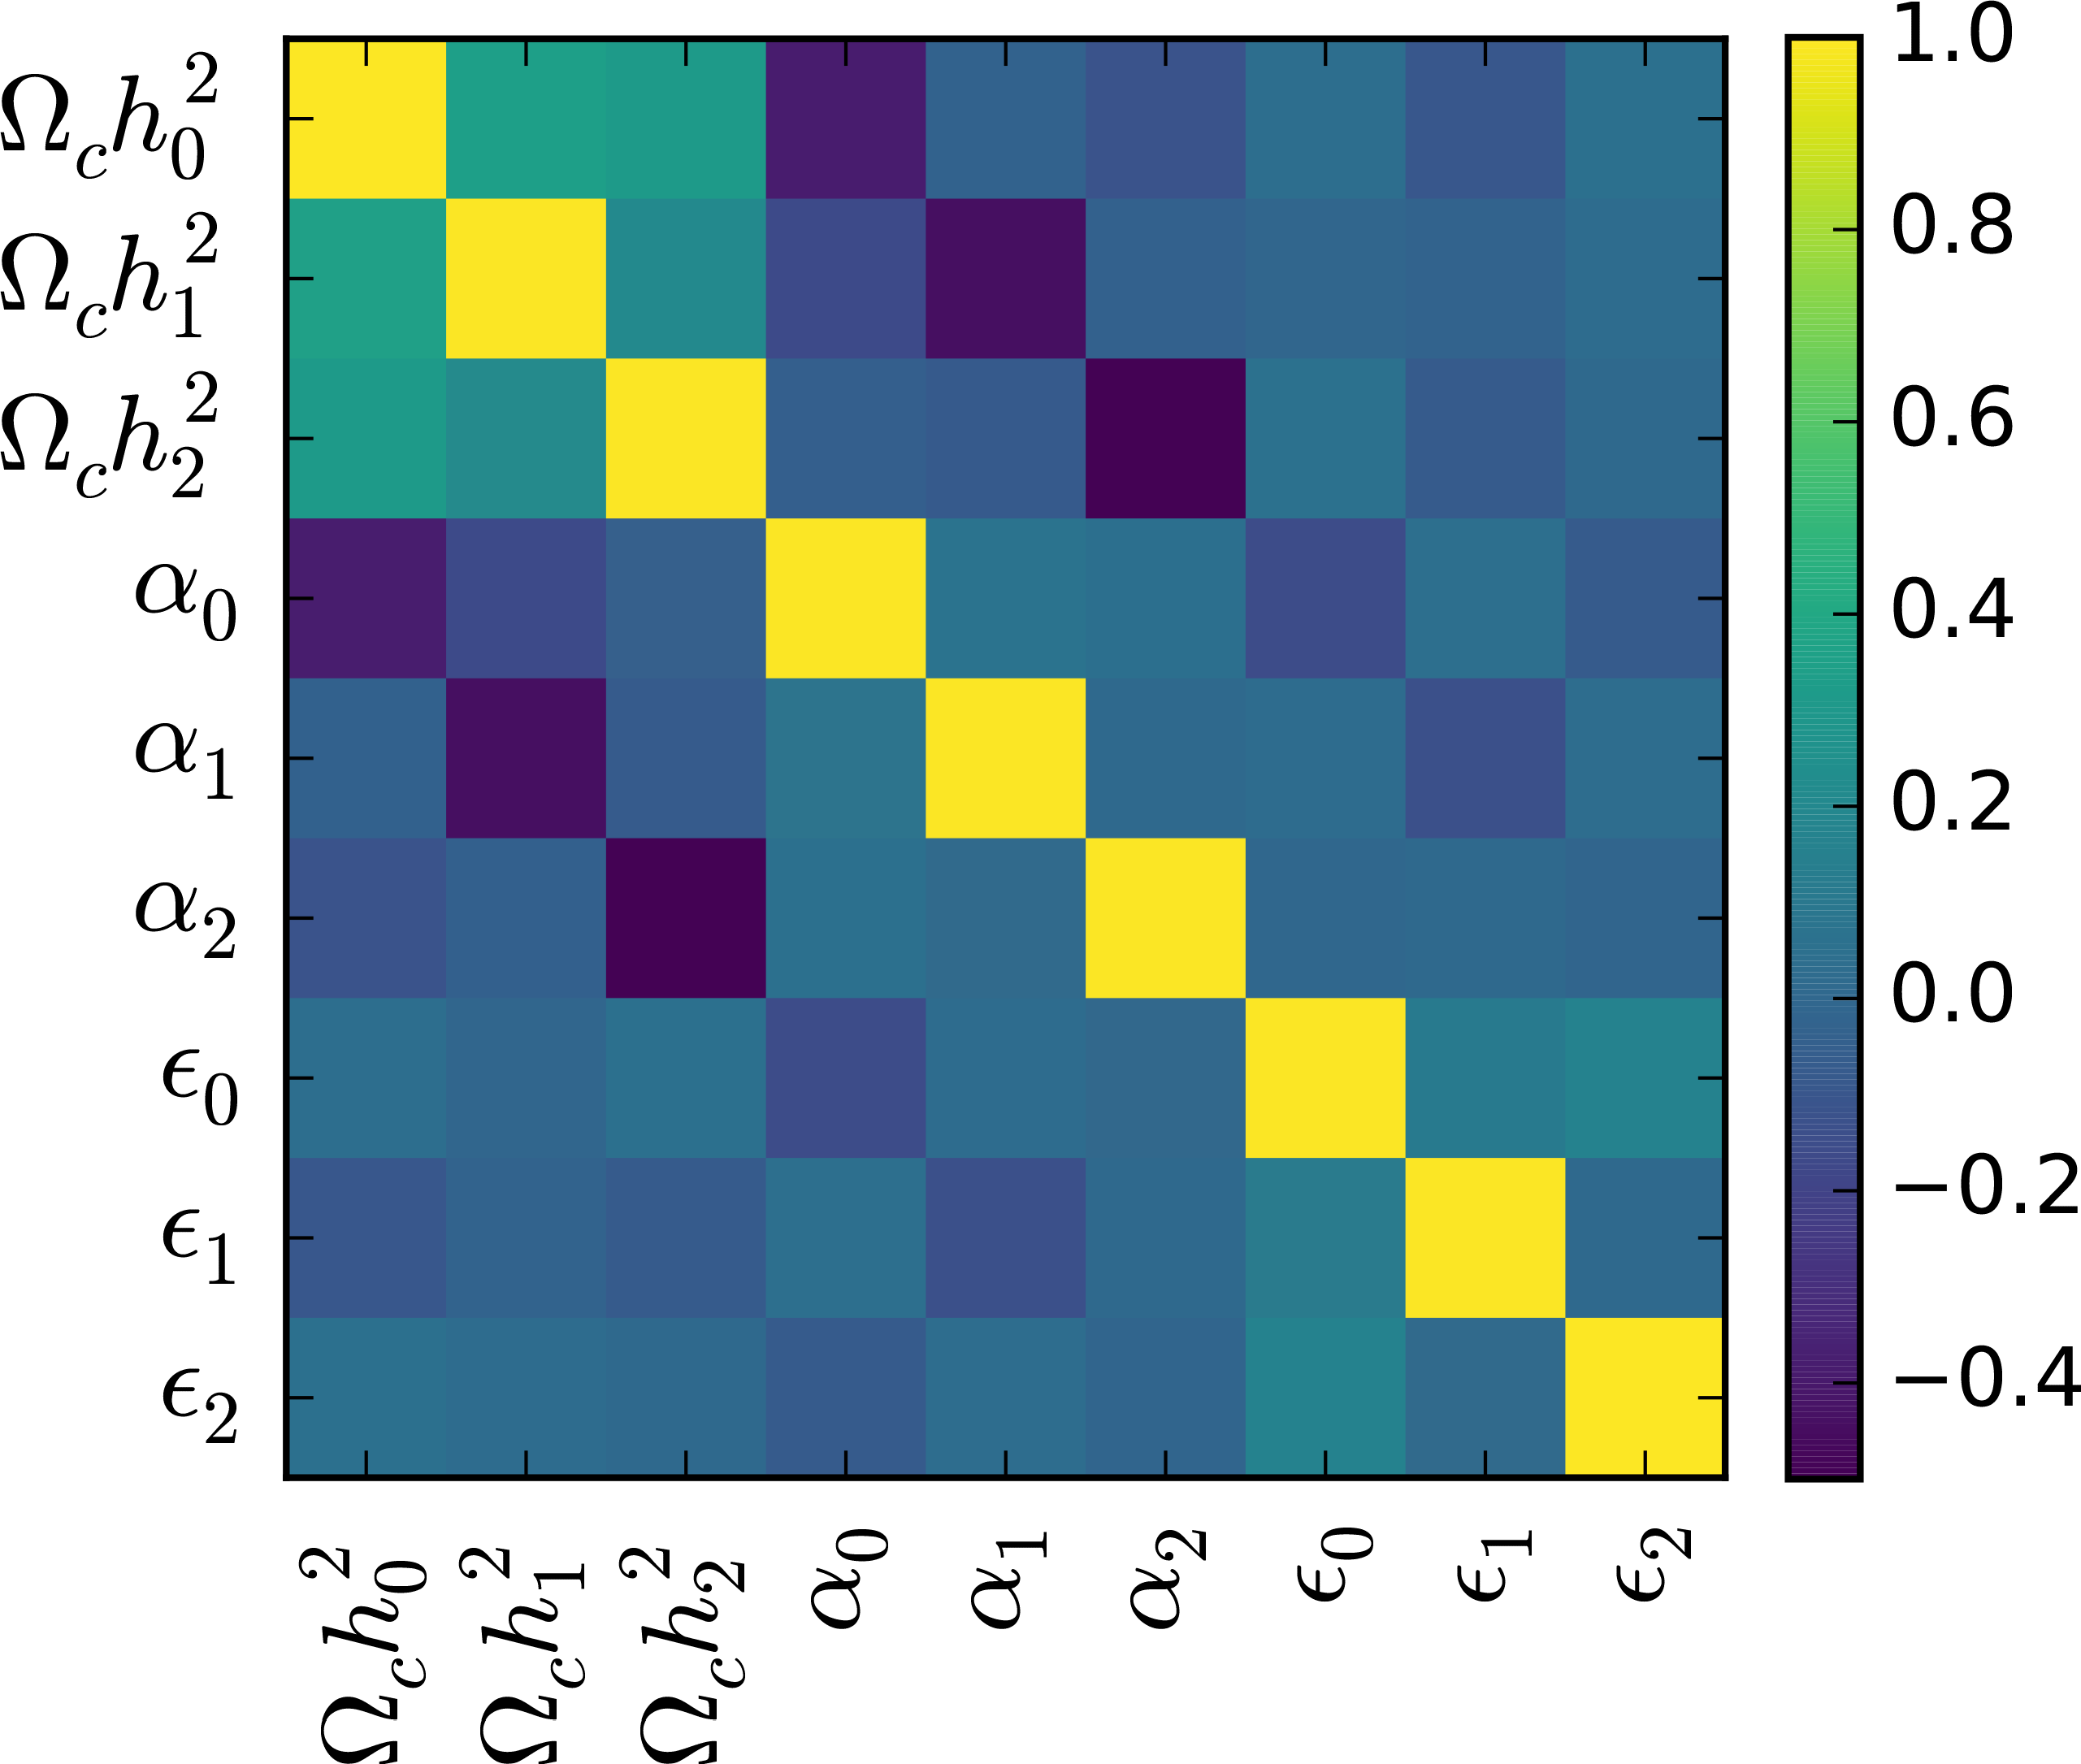
\includegraphics[width=0.85\columnwidth]{images/correlations.png}
	\end{center}
	\caption{Correlations between final cosmological parameters when fitting to the three redshift bins of each WizCOLA simulation for the multipole data. The subscript numbers after each parameter are used to denote the redshift bin, with $0$, $1$, and $2$ respectively denoting the $0.2 < z < 0.6$, $0.4 < z < 0.8$, and $0.6 < z < 1.0$ bins. }
	\label{fig:correlations}
	%\end{wrapfigure}
\end{figure}
\begin{figure}[t]
	%\begin{wrapfigure}{r}{0.5\textwidth}
	\begin{center}
		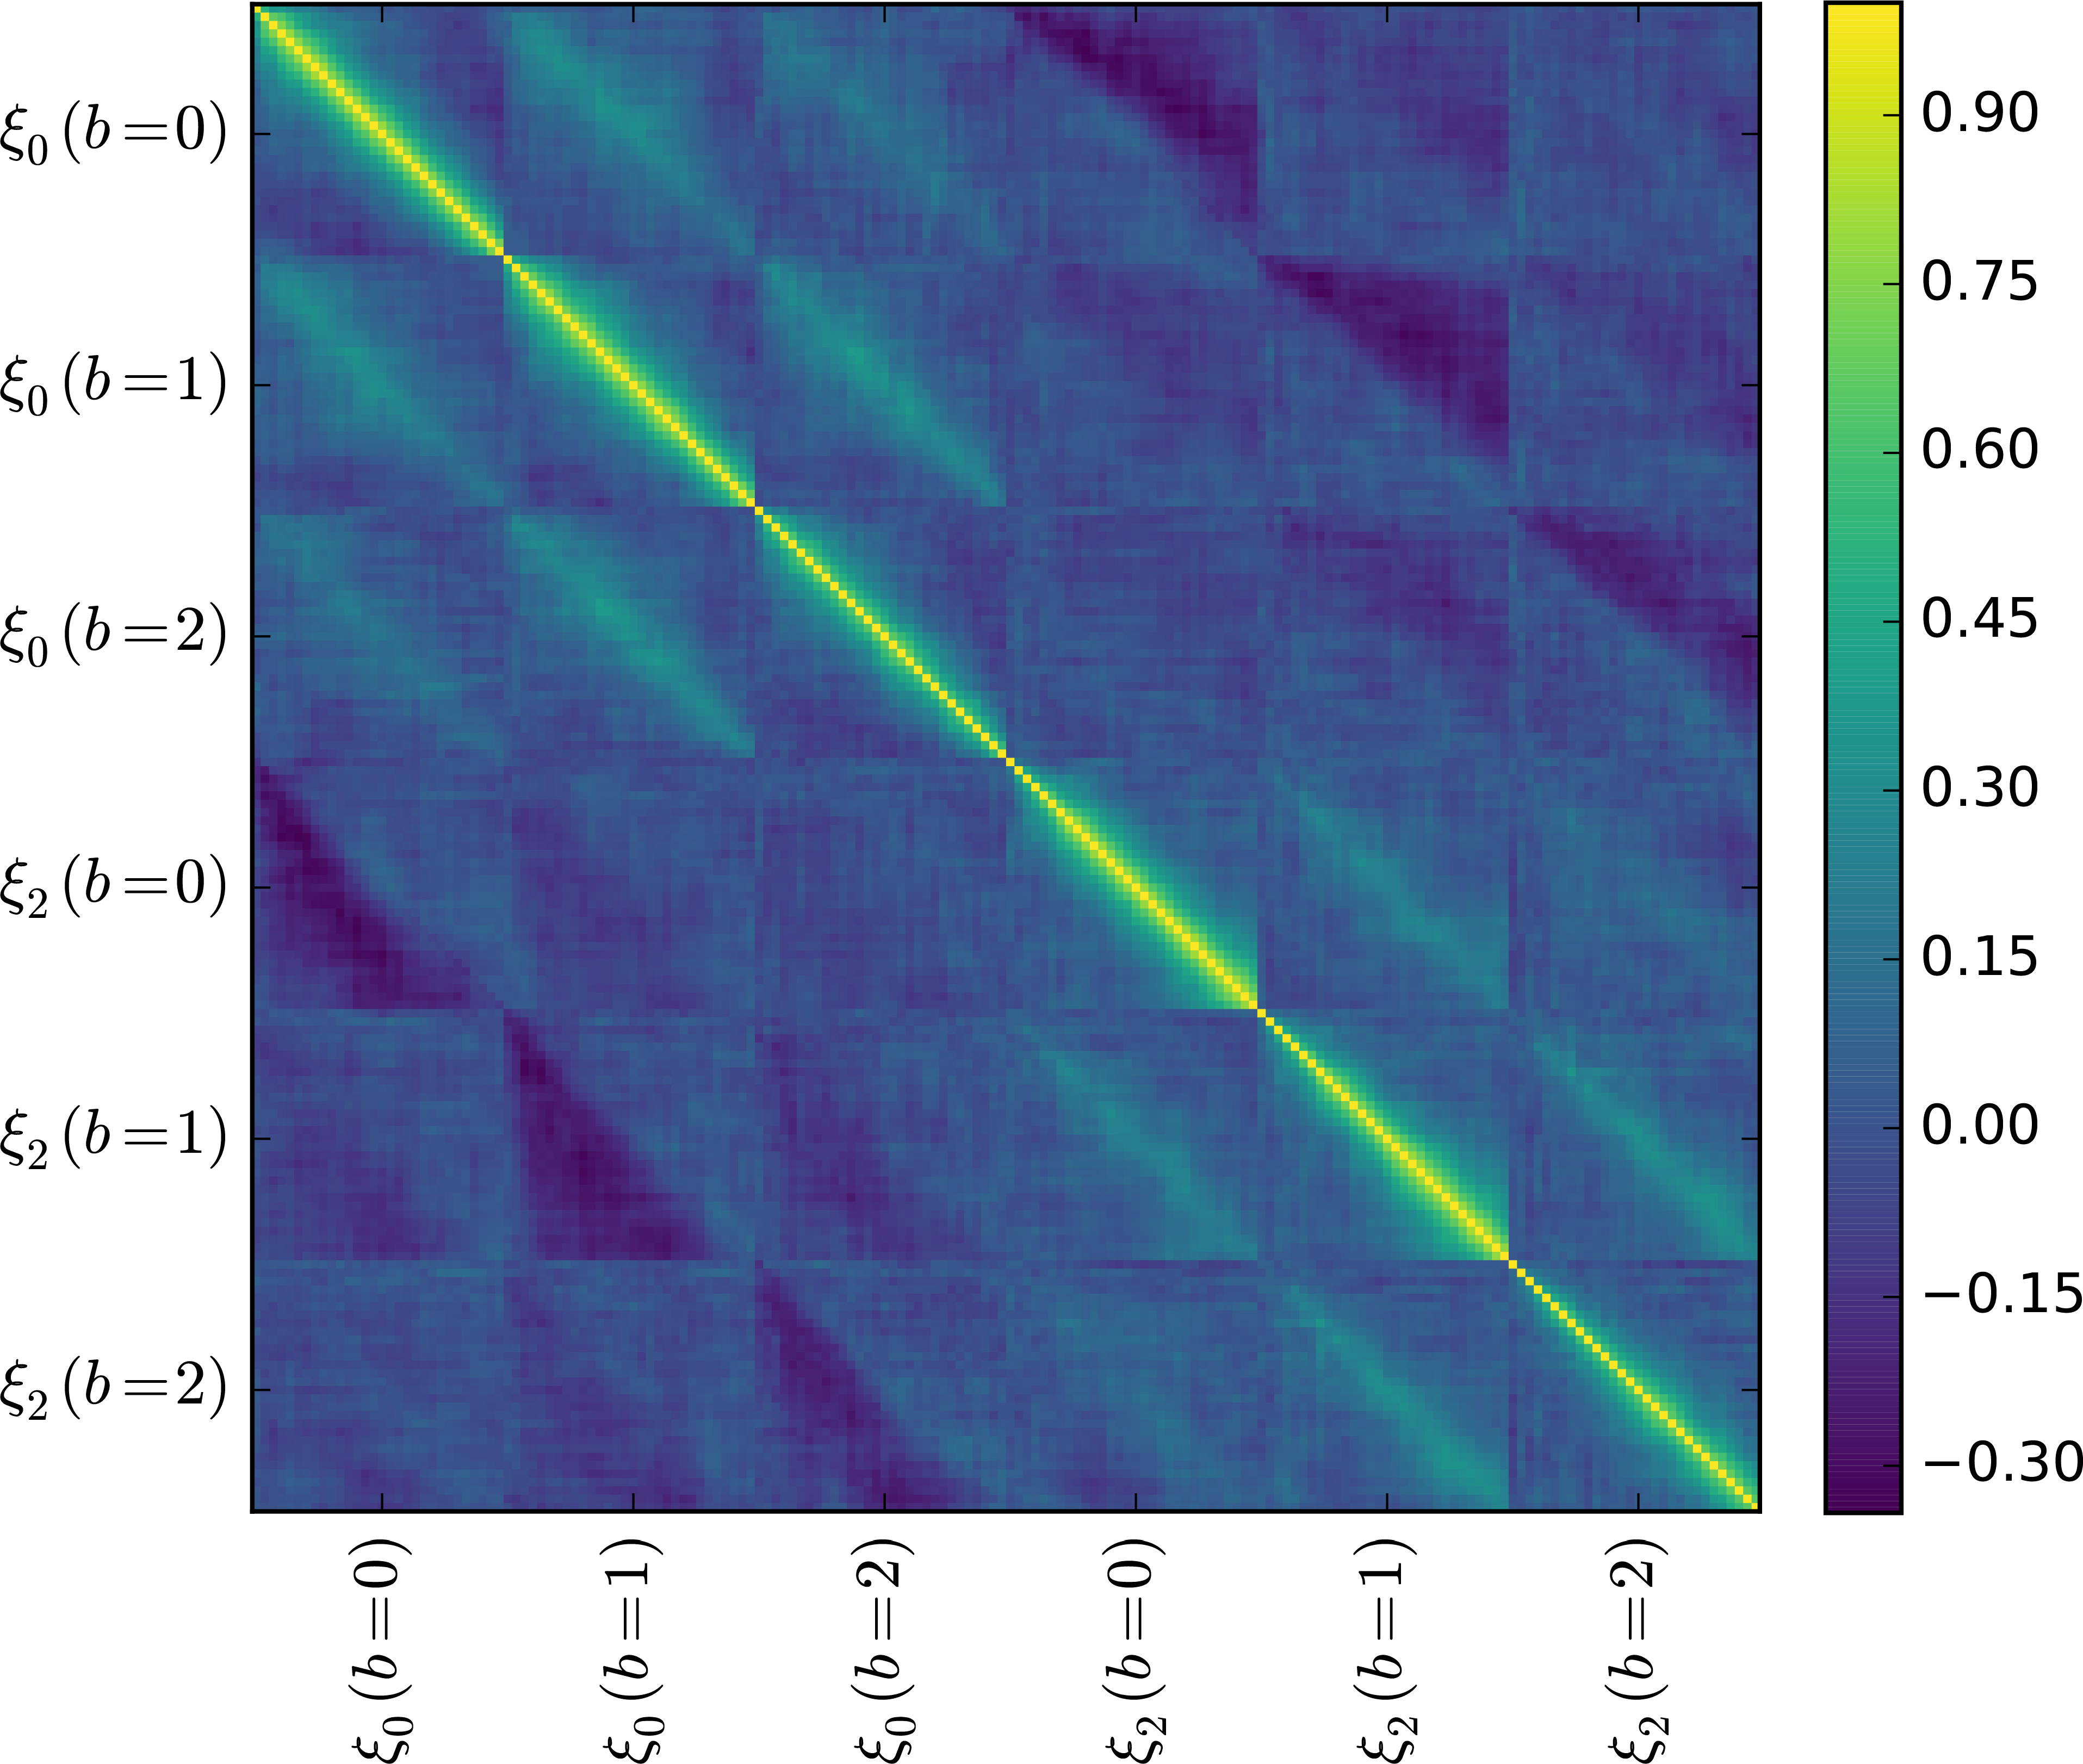
\includegraphics[width=\columnwidth]{images/fullCorrelations.png}
	\end{center}
	\caption{Full data correlation matrices constructed for both the multipole expression of the WizCOLA data. The $b=0$, $b=1$ and $b=2$ labels respectively refer to the redshift bins $0.2 < z < 0.6$, $0.4 < z < 0.8$ and $0.6 < z < 1.0$. We can see that, even though the $b=0$ and $b=2$ bins do not overlap, some faint correlation still persists. This is expected, as long modes in the simulation would span both bins.}
	\label{fig:fullCorrelations}
	%\end{wrapfigure}
\end{figure}




This covariance matrix can now be used to fit for a final $\Omega_c h^2$, $\alpha$ and $\epsilon$, %(for a multipole analysis), %or a final $\Omega_c h^2$, $\alpha_\perp$ and $\alpha_\parallel$ (for a wedge analysis). 
%Treating only multipoles hereonin to simplify the text, this is done 
by  minimising the $\chi^2$ statistic, given as,
\begin{align} \label{eq:covchi}
\chi^2(\Omega_c h^2, \alpha, \epsilon) &= (\Omega_c h^2 - \Omega_c h^2_0, \Omega_c h^2 - \Omega_c h^2_1, ...,\  \epsilon - \epsilon_2)^T \notag \\
 &C_{ij}^{-1}(\Omega_c h^2 - \Omega_c h^2_0, \Omega_c h^2 - \Omega_c h^2_1, ...,\  \epsilon - \epsilon_2),
\end{align}
where again the subscript indices on the $\Omega_c h^2$, $\alpha$ and $\epsilon$ refer to the redshift bins. In essence, we utilise the parameters fitted to each bin as datapoints in a secondary model, which we minimise with respect to the final parameters $\Omega_c h^2$, $\alpha$ and $\epsilon$.




\subsubsection{Second method: All data covariance} \label{sec:allData}

The covariance matrices utilised so far in our analysis have been supplied from the WizCOLA simulations, and give data covariance inside each redshift bin. However, also having the 600 WizCOLA realisations, we can reconstruct a full covariance matrix to give the covariance between values of the correlation function across redshift bins. The correlation matrices for the multipole data are shown in Figure \ref{fig:fullCorrelations}.




When using the full data covariance to simultaneously fit all three redshift bins, a further question becomes whether marginalisation parameters $b^2$, $\beta$, $\sigma_V$ and $k_*$ should be free between redshift bins, or consistent across them. 

From a physical motivation, we expect the bias parameter $b^2$ to be dependent on redshift bin. This is because we only observe the most massive, luminous galaxies at high redshift, which have higher bias than the less massive galaxies we can see at lower redshifts. However, when performing fits, $b^2$ and $\beta$ are well constrained, whilst $k_*$ and $\sigma_V$ are not. As this implies that those two parameters do not significantly contribute to the likelihood calculations, it is unknown if setting $\sigma_V$ free between bins will have a noticeable benefit. 


To investigate this, we ran fits to the combined WizCOLA data where we set no nuisance parameters free between redshift bins, when we only set $b^2$ free, when we set all \textit{but} $b^2$ free, and then when we set all four nuisance parameters free.  These fits indicate a strong preference for fitting with separate $b^2$ values in different redshift bins due to tighter constraints achieved, and an accompanying improvement in $\chi^2$.  However allowing the other nuisance parameters to vary between redshift bins has negligible benefits (it neither increases fit strength nor removes  bias), and adds computational time in the form of delayed chain convergence.

Based on these results, we utilise independent $b^2$ values, whilst fixing $\beta$, $\sigma_v$ and $\sigma_V$ between bins when fitting with the full data set and full data covariance.
% A comparison of their likelihood distributions is shown in Figure \ref{fig:wizcolaAllNormalCovCombined}.
\begin{comment}
\begin{figure}
	\begin{center}
		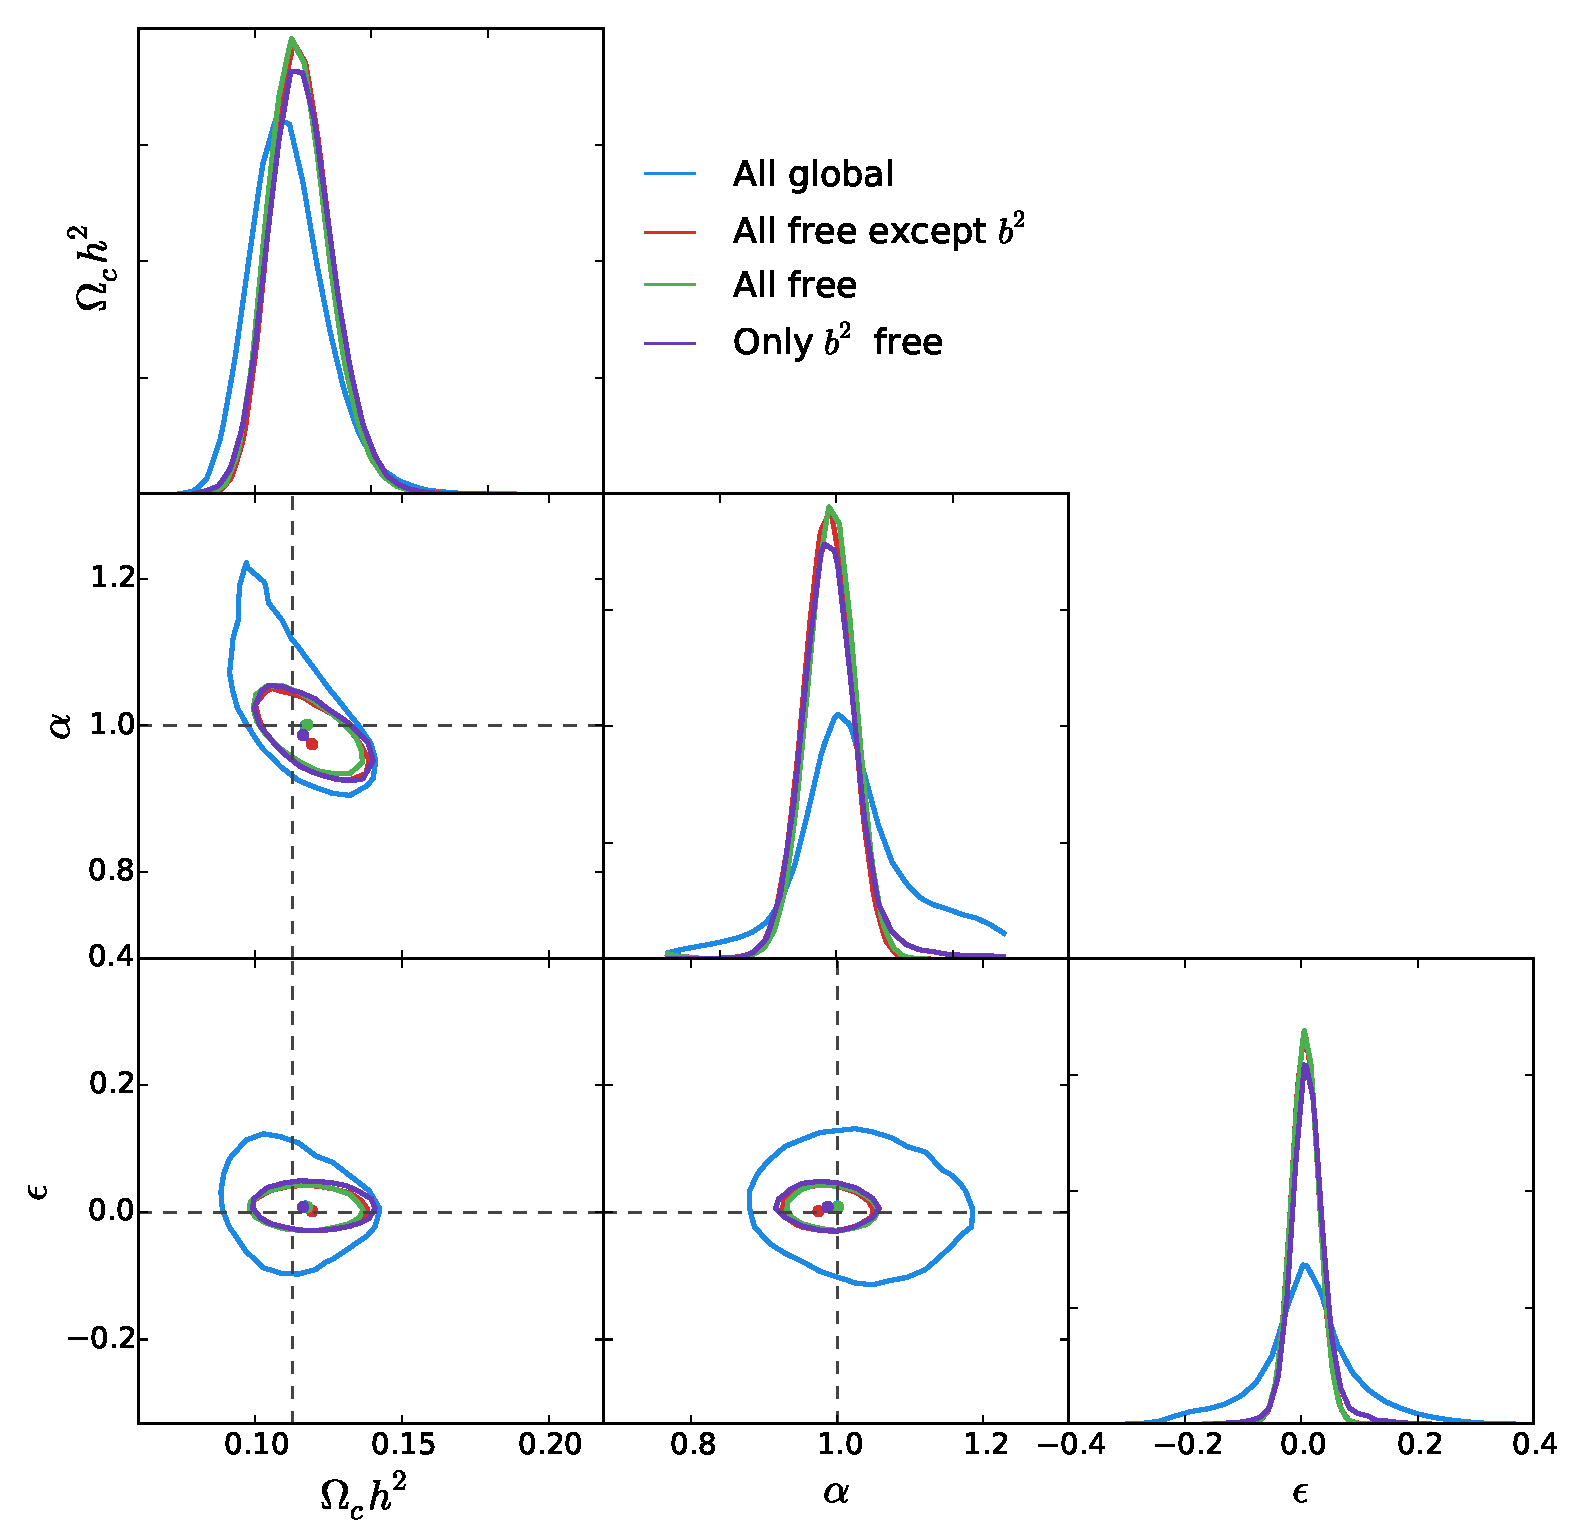
\includegraphics[width=\columnwidth]{images/wizcolaAllNormalCovCombined.pdf}
	\end{center}
	\caption{Fits to the mean WizCOLA data using the computed covariance matrix. Marginalisation parameters for the fit are $b^2$, $\beta$, $\sigma_v$ and $\sigma_V$. There are four fits shown, where the word `free' has been used to indicate that the parameter in question has been allowed to take different values for each redshift bin. We can see that allowing $b^2$ to vary improves the tightness of the fit, but it is the only nuisance parameter that appears to need redshift dependence.}
	\label{fig:wizcolaAllNormalCovCombined}
\end{figure}
\end{comment}


\subsection{Multipole model testing conclusions}

%In this chapter we have sought to validate our constructed BAO model. The one dimensional base model was first validated by successfully reproducing fits to the one dimensional WiggleZ survey as found in \citet{BlakeDavis2011} and \citet{BlakeKazin2011} to within a $1\sigma$ limit. Both methodologies for incorporating angular dependence to create a 2D BAO model, by modelling data wedges or multipole expansion, were then successfully tested using the combined WizCOLA simulation dataset by recovering the simulation parameters. Failure of the $\alpha_\parallel$ parameter to consistently converge led to us discarding the wedge analysis. The significance of the hexadecapole term for the multipole data was investigated, and was found to be small enough that discarding the term for computational benefit would have a negligible impact on parameter recovery when compared to statistical error.\\

%Due to the overlapping redshift bins in the analyses, covariance between the final cosmological parameters was determined by comparing individual realisations of the WizCOLA simulations, and this will be used in conjunction with an analysis using the all data across redshift bins to get global parameters. 

 A graphical comparison of fits to the mean WizCOLA data for individual redshift bins, all data fits, and combining bin parameters can be found for the multipole data format in Figure \ref{fig:corCombinedMPWiz}. 
 The results are consistent between bins, and between methods of combining bins, and all are consistent with the input cosmology.  We therefore conclude that our model can accurately be used to derive cosmological constraints from WiggleZ-like data.  The results with real data are presented in Section~\ref{sec:multi}, but before presenting these results we continue our validation testing, now on the reconstructed data. 


%Having performed various tests to determine that our constructed models is free of significant bias and is able to correctly recover cosmological values, we will now apply the model to the WiggleZ data. 





\begin{figure}[h!]
	%%\begin{wrapfigure}{r}{0.5\textwidth}
	\begin{center}
		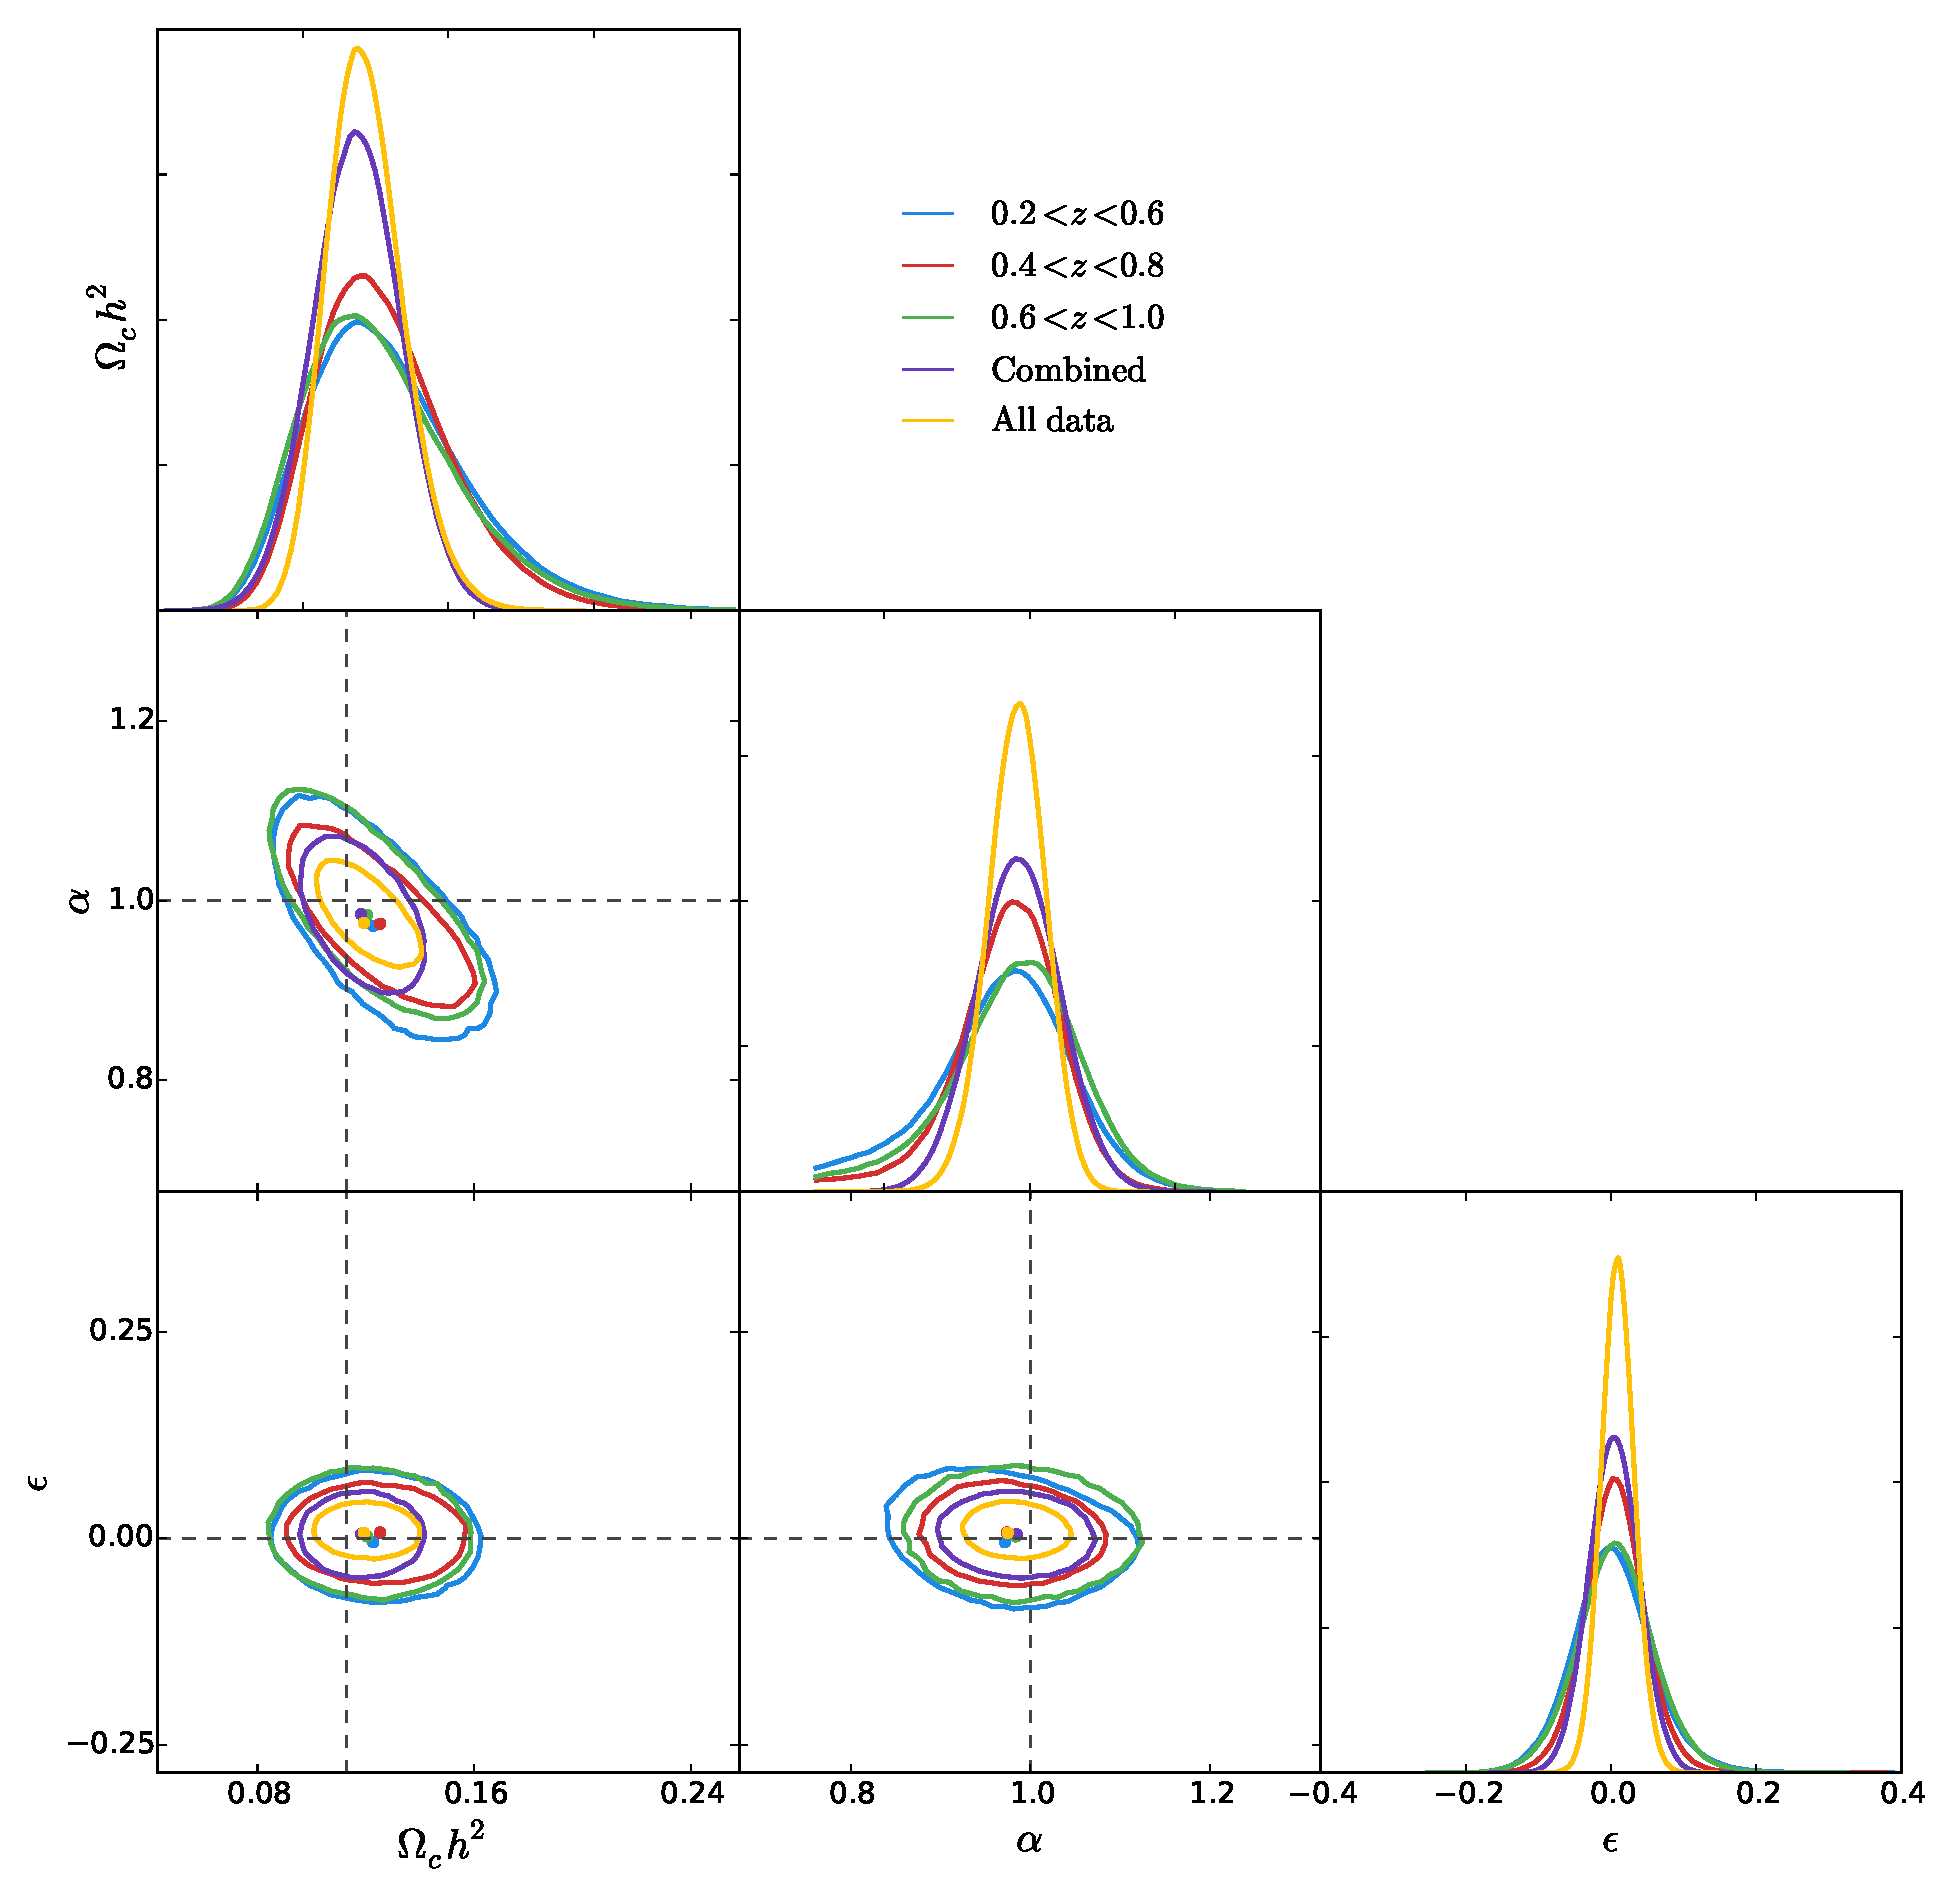
\includegraphics[width=\columnwidth]{images/corCombinedMPWiz.pdf}
	\end{center}
	\caption{Fits to the mean data of all 600 WizCOLA realisations %(without reducing data uncertainty) 
	for the multipole expansion expression of the data. Fits using all three bins simultaneously are shown as the ``All data'' fits, and the combination of maximum likelihood parameters using parameter covariance is shown as the ``Combined'' likelihood surfaces. In all cases we recover simulation cosmology well within $1\sigma$ limits.}
	\label{fig:corCombinedMPWiz}
	%\end{wrapfigure}
\end{figure}

%\begin{figure}[h!]
%	%%\begin{wrapfigure}{r}{0.5\textwidth}
%	\begin{center}
%		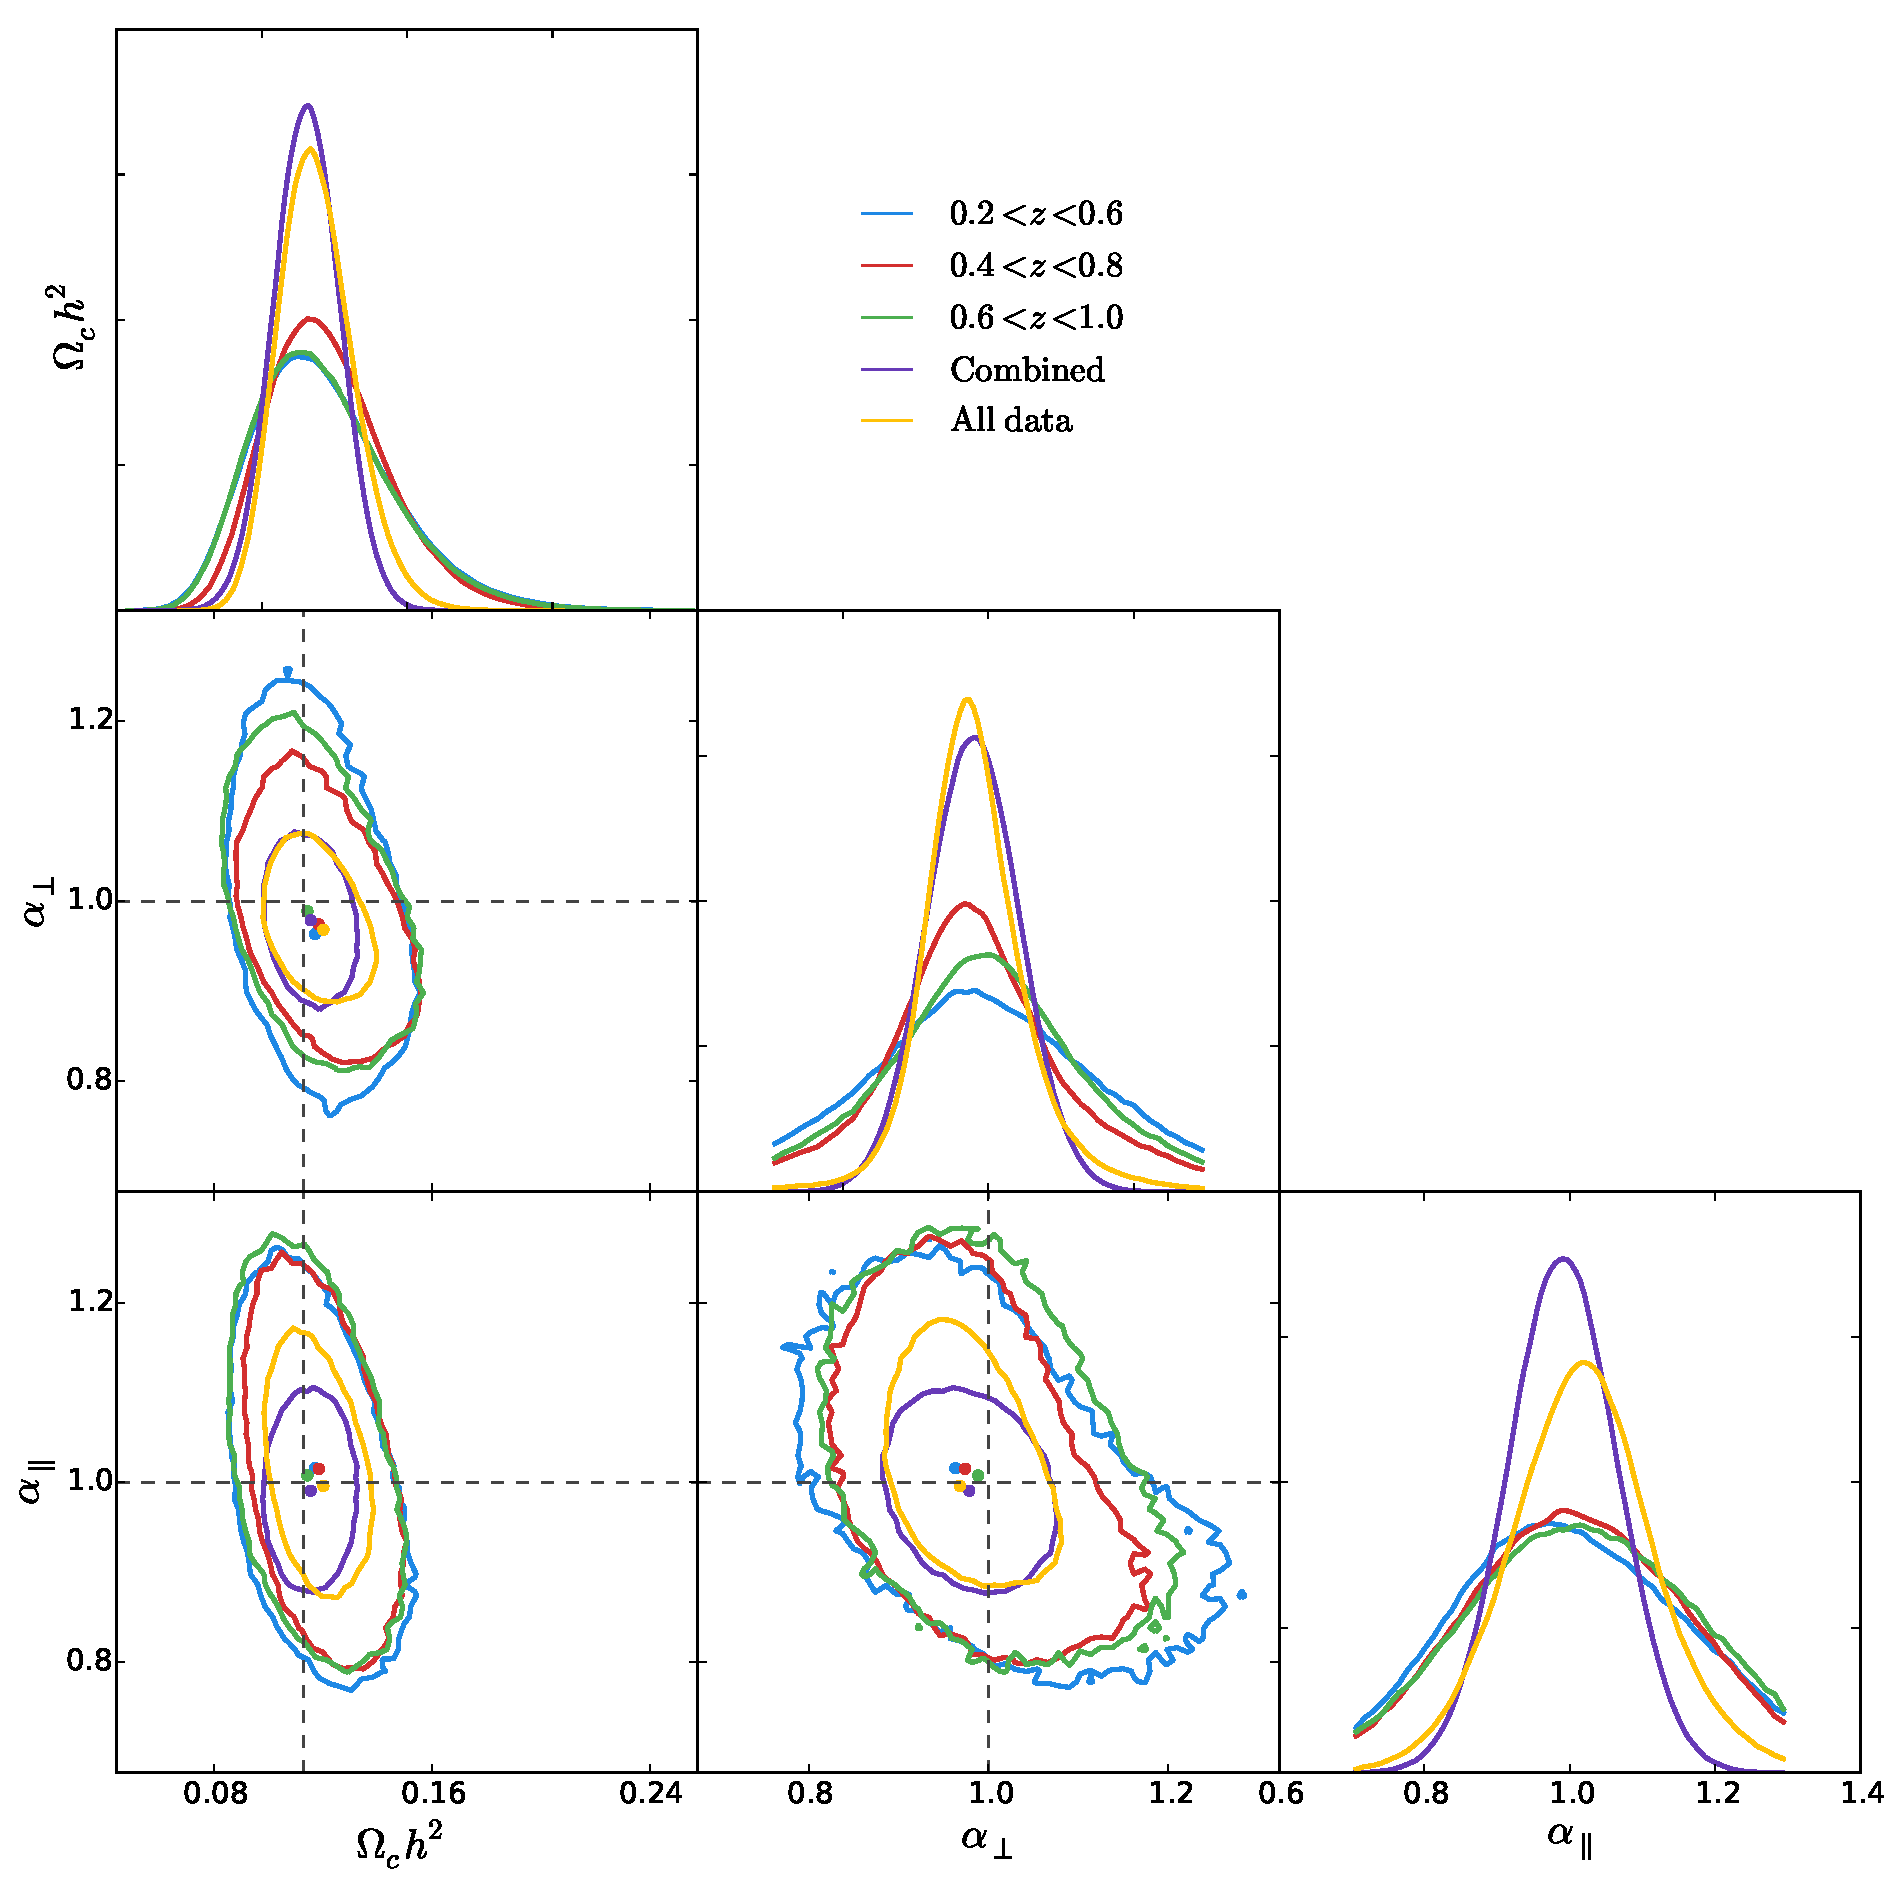
\includegraphics[width=\columnwidth]{images/corCombinedWedgeWiz.pdf}
%	\end{center}
%	\caption{Fits to the mean data of all 600 WizCOLA realisations (without reducing data uncertainty) for the wedge expansion expression of the data. Fits using all three bins simultaneously are shown as the ``All data'' fits, and the combination of maximum likelihood parameters using parameter covariance is shown as the ``Combined'' likelihood surfaces. In all cases we recover simulation cosmology well within $1\sigma$ limits, although we should note that the data strength is not significant enough to constrain $\alpha_\parallel$ to the $2\sigma$ limits even in this optimal example (where the data input is the mean of all 600 realisations).}
%	\label{fig:corCombinedWedgeWiz}
%	%\end{wrapfigure}
%\end{figure}



\section{Validating reconstructed wedge data}

For the reconstructed data that we analyse in wedges we also tested our procedure using the WiZCOLA mock catalogues.  We focus
here on results from the mocks of the $\Delta z^{\rm Far}$ redshift
slice, which are representative of the behaviour in all redshift bins.
In Figure \ref{fig:wizcola_hdaModes_z60_epsilonT15} we present the
best-fitting values of $\alpha_\parallel$ and $\alpha_\perp$ from each
of the 600 simulations, and in Figure
\ref{fig:wizcola_hdaUnc_z60_epsilonT15} we show the corresponding
uncertainties.  The uncertainties are typically large, indicating a
marginal detection of the baryon acoustic peak in the clustering
wedges.  This motivated us to consider, in addition to the $50\%$
priors on $\alpha_\parallel$ and $\alpha_\perp$ mentioned above,
additional flat priors on their combination, which we parameterize as
$\alpha = \alpha_\perp^{2/3} \alpha_\parallel^{1/3} \sim D_{\rm
  A}^2 r^\prime_s /(H r_s)$ and $\epsilon = (\alpha_\parallel/\alpha_\perp)^{1/3} - 1
\sim 1/(D_{\rm A} H)$.
The $\alpha$ parameter is mostly sensitive to
the monopole and $\epsilon$ to the quadrupole, although both terms appear in all
multipoles \citep[see][for a discussion]{PadmanabhanWhite2008}. In the
final analysis we applied a $15\%$ flat prior on $\epsilon$, which is
marked by the red dot-dashed lines in Figure
\ref{fig:wizcola_hdaModes_z60_epsilonT15}.  We did not apply a prior
in $\alpha$, but for illustration we show the $\pm 25\%$ threshold as
the blue dashed lines in Figure
\ref{fig:wizcola_hdaModes_z60_epsilonT15}.  We selected from the 600
realizations those that have a significance of BAO detection equal to
or greater than that in the real dataset ($2.9\sigma$).  We find 87
such mocks (15\%; marked as large blue circles).  In Figure
\ref{fig:wizcola_hdaUnc_z60_epsilonT15} we also show our WiggleZ
$\Delta z^{\rm Far}$ result with a yellow star.

Many WiggleZ mock realizations do not permit good constraints on both
$\alpha_\perp$ and $\alpha_\parallel$.  However, for the subset of
realizations with similar detection significance to the WiggleZ data,
we find that our procedure enables us to extract unbiased distance
measurements, with median and standard deviations $\langle \alpha_\perp \rangle =
1.001 \pm 0.081$ and $\langle \alpha_\parallel \rangle = 0.999 \pm 0.154$.  The
median and standard deviation of the errors in these parameters, for
this subset of mocks, are $<\sigma_{\alpha_\perp}> = 0.052 \pm 0.037$
and $\langle \sigma_{\alpha_\parallel} \rangle = 0.107 \pm 0.061$.  Similar results
are obtained when analyzing mocks at $\Delta z^{\rm Mid}$ and $\Delta
z^{\rm Near}$.  In all cases, the results for the WiggleZ data are
consistent with range covered by the simulations.

We now consider the degree to which our $15\%$ prior in $\epsilon$
impacts the model-independence of our results.  Using MCMC chains
based on {\sl Planck} temperature and {\sl WMAP} polarization data, we
found that the scatter in $\epsilon$ at our redshifts of interest was
$2.0\%$ for a flat $\Lambda$CDM model and $2.5\%$ for an $ow$CDM
model.  We hence argue that our much larger $15\%$ prior does not
significantly compromise our model-independence.

\begin{figure}
\begin{center}
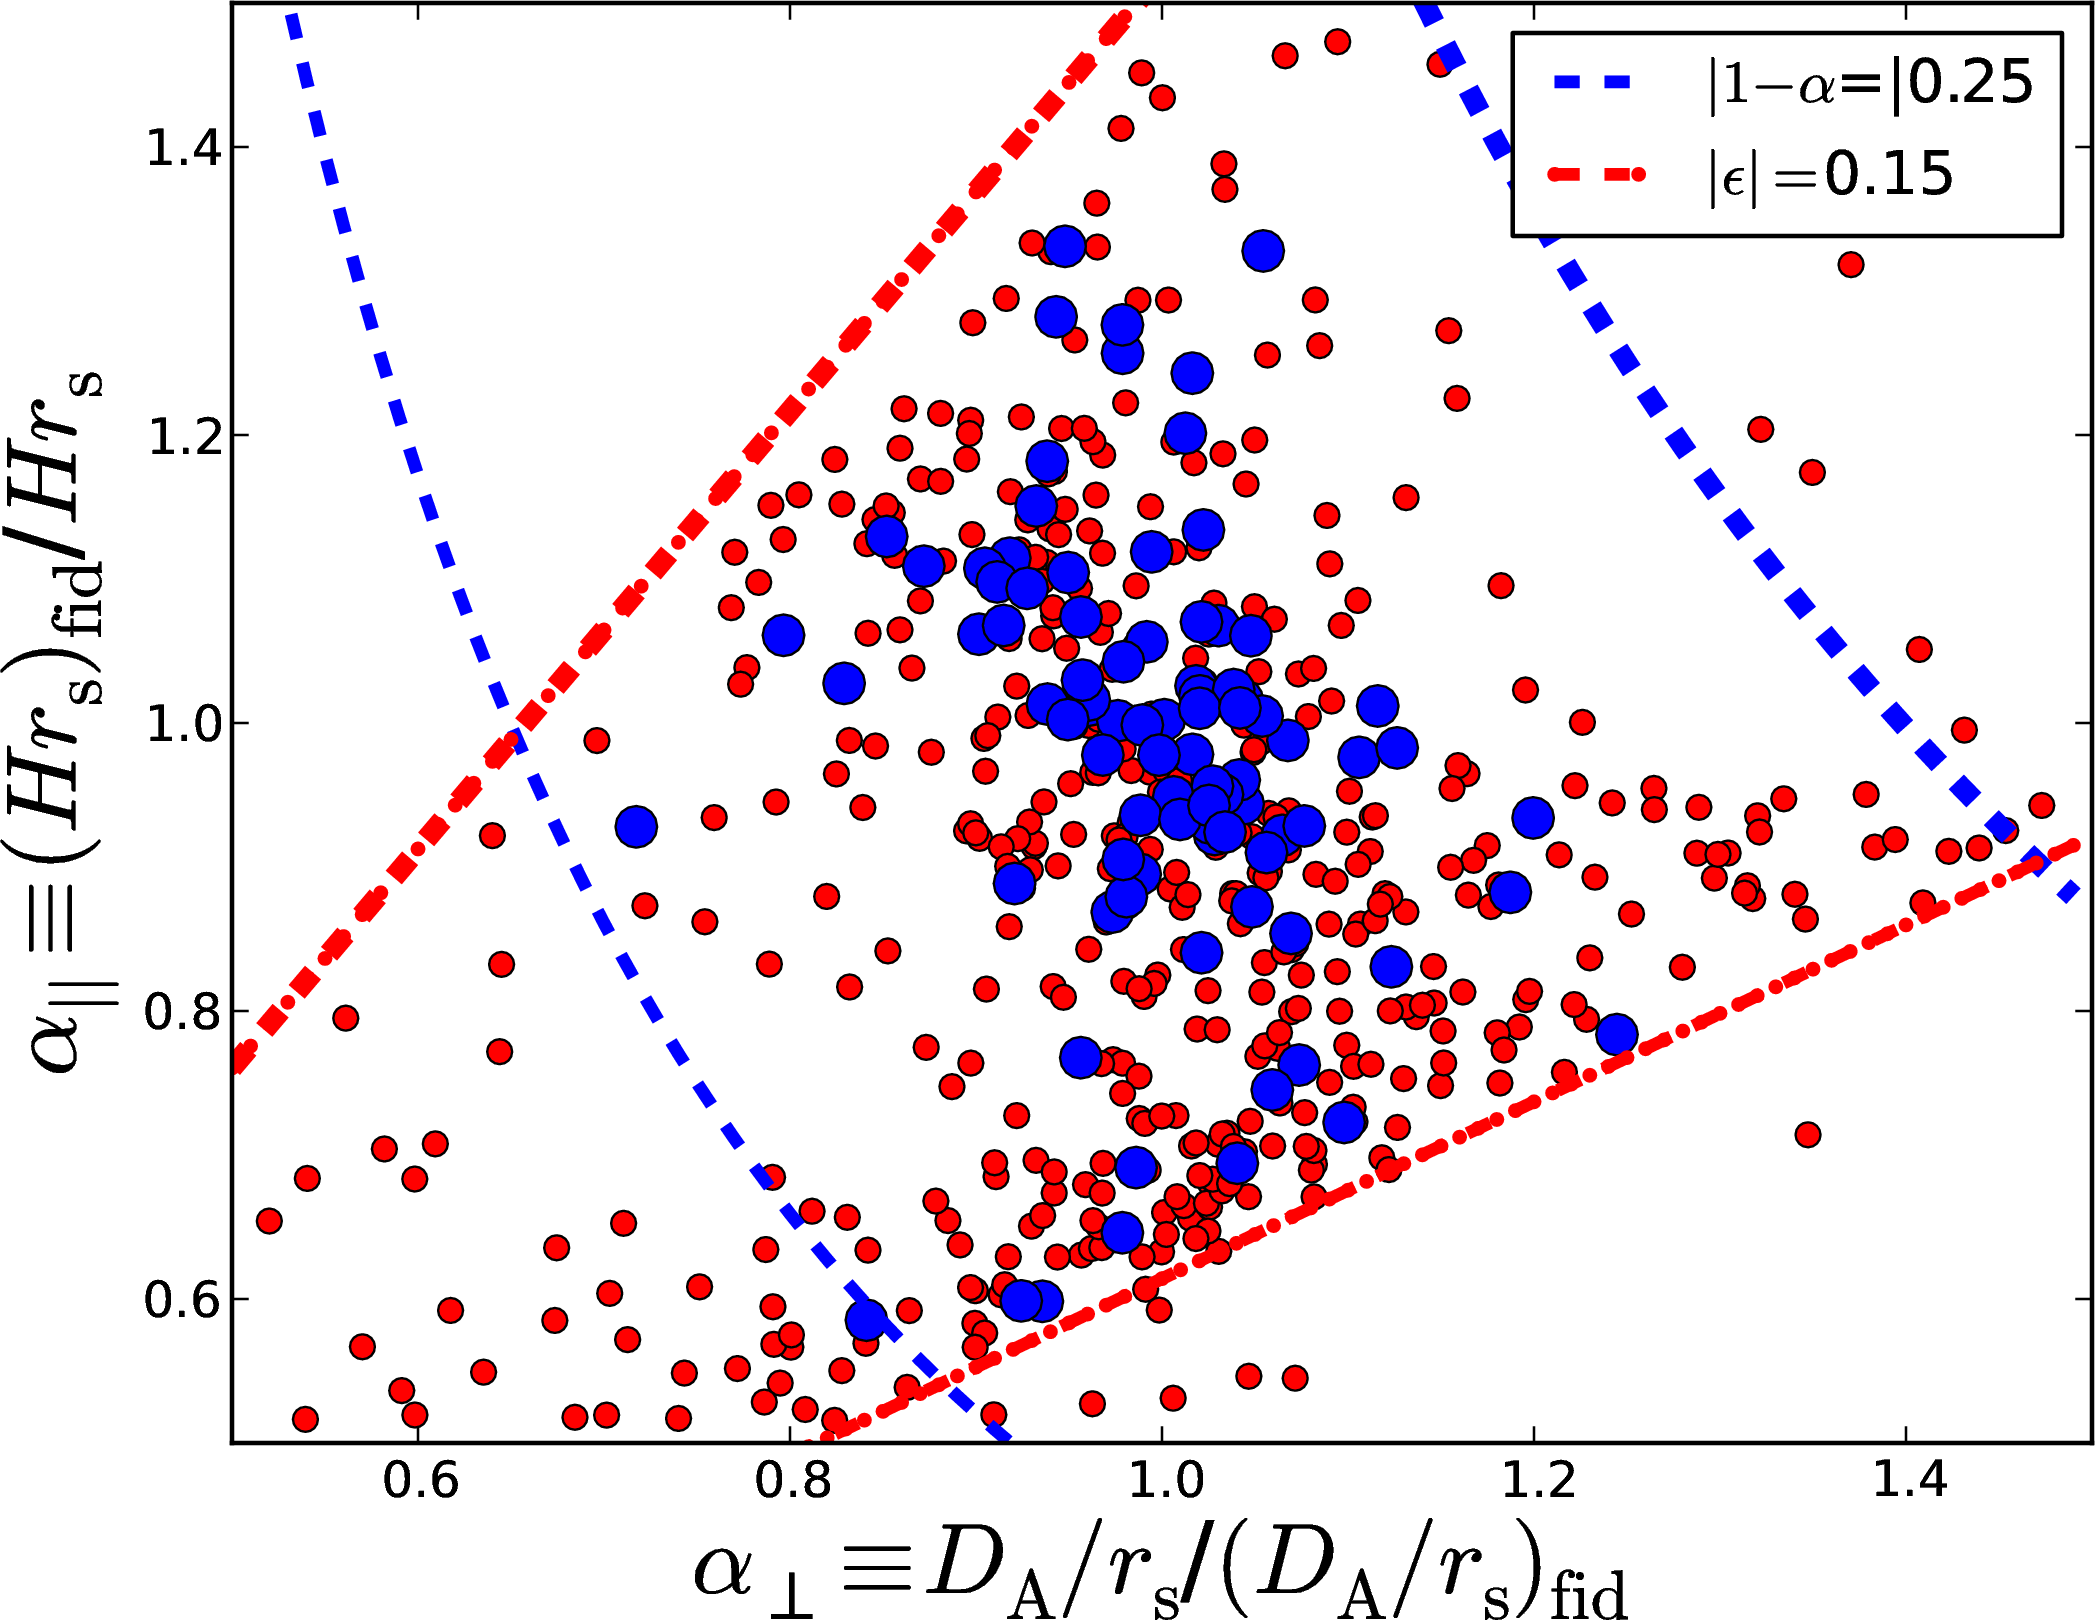
\includegraphics[width=0.7\columnwidth]{figures/WiZCOLA_mode_z0pt6_1pt0/WiZCOLA_mode_z0pt6_1pt0}
\caption{\label{fig:wizcola_hdaModes_z60_epsilonT15} WiZCOLA $0.6<z<1$ $\alpha_{||}$ and $\alpha_\perp$ mode results. The large blue circles (87/600) are realizations that have a significance of detection of 2.9$\sigma$ (as the observation) or higher. The red are below this threshold. The red dot-dashed lines mark the $\pm15\%$ value of the fiducial $\epsilon$ which we use as a flat prior in this calculation. The dashed blue lines mark $\pm25\%$ of the fiducial $\alpha$, but are just for visualisation as we did not apply these as a prior. The thicker lines indicate the higher values of the $\alpha$ and $\epsilon$ limits.%
}
\end{center}
\end{figure}

\begin{figure}
\begin{center}
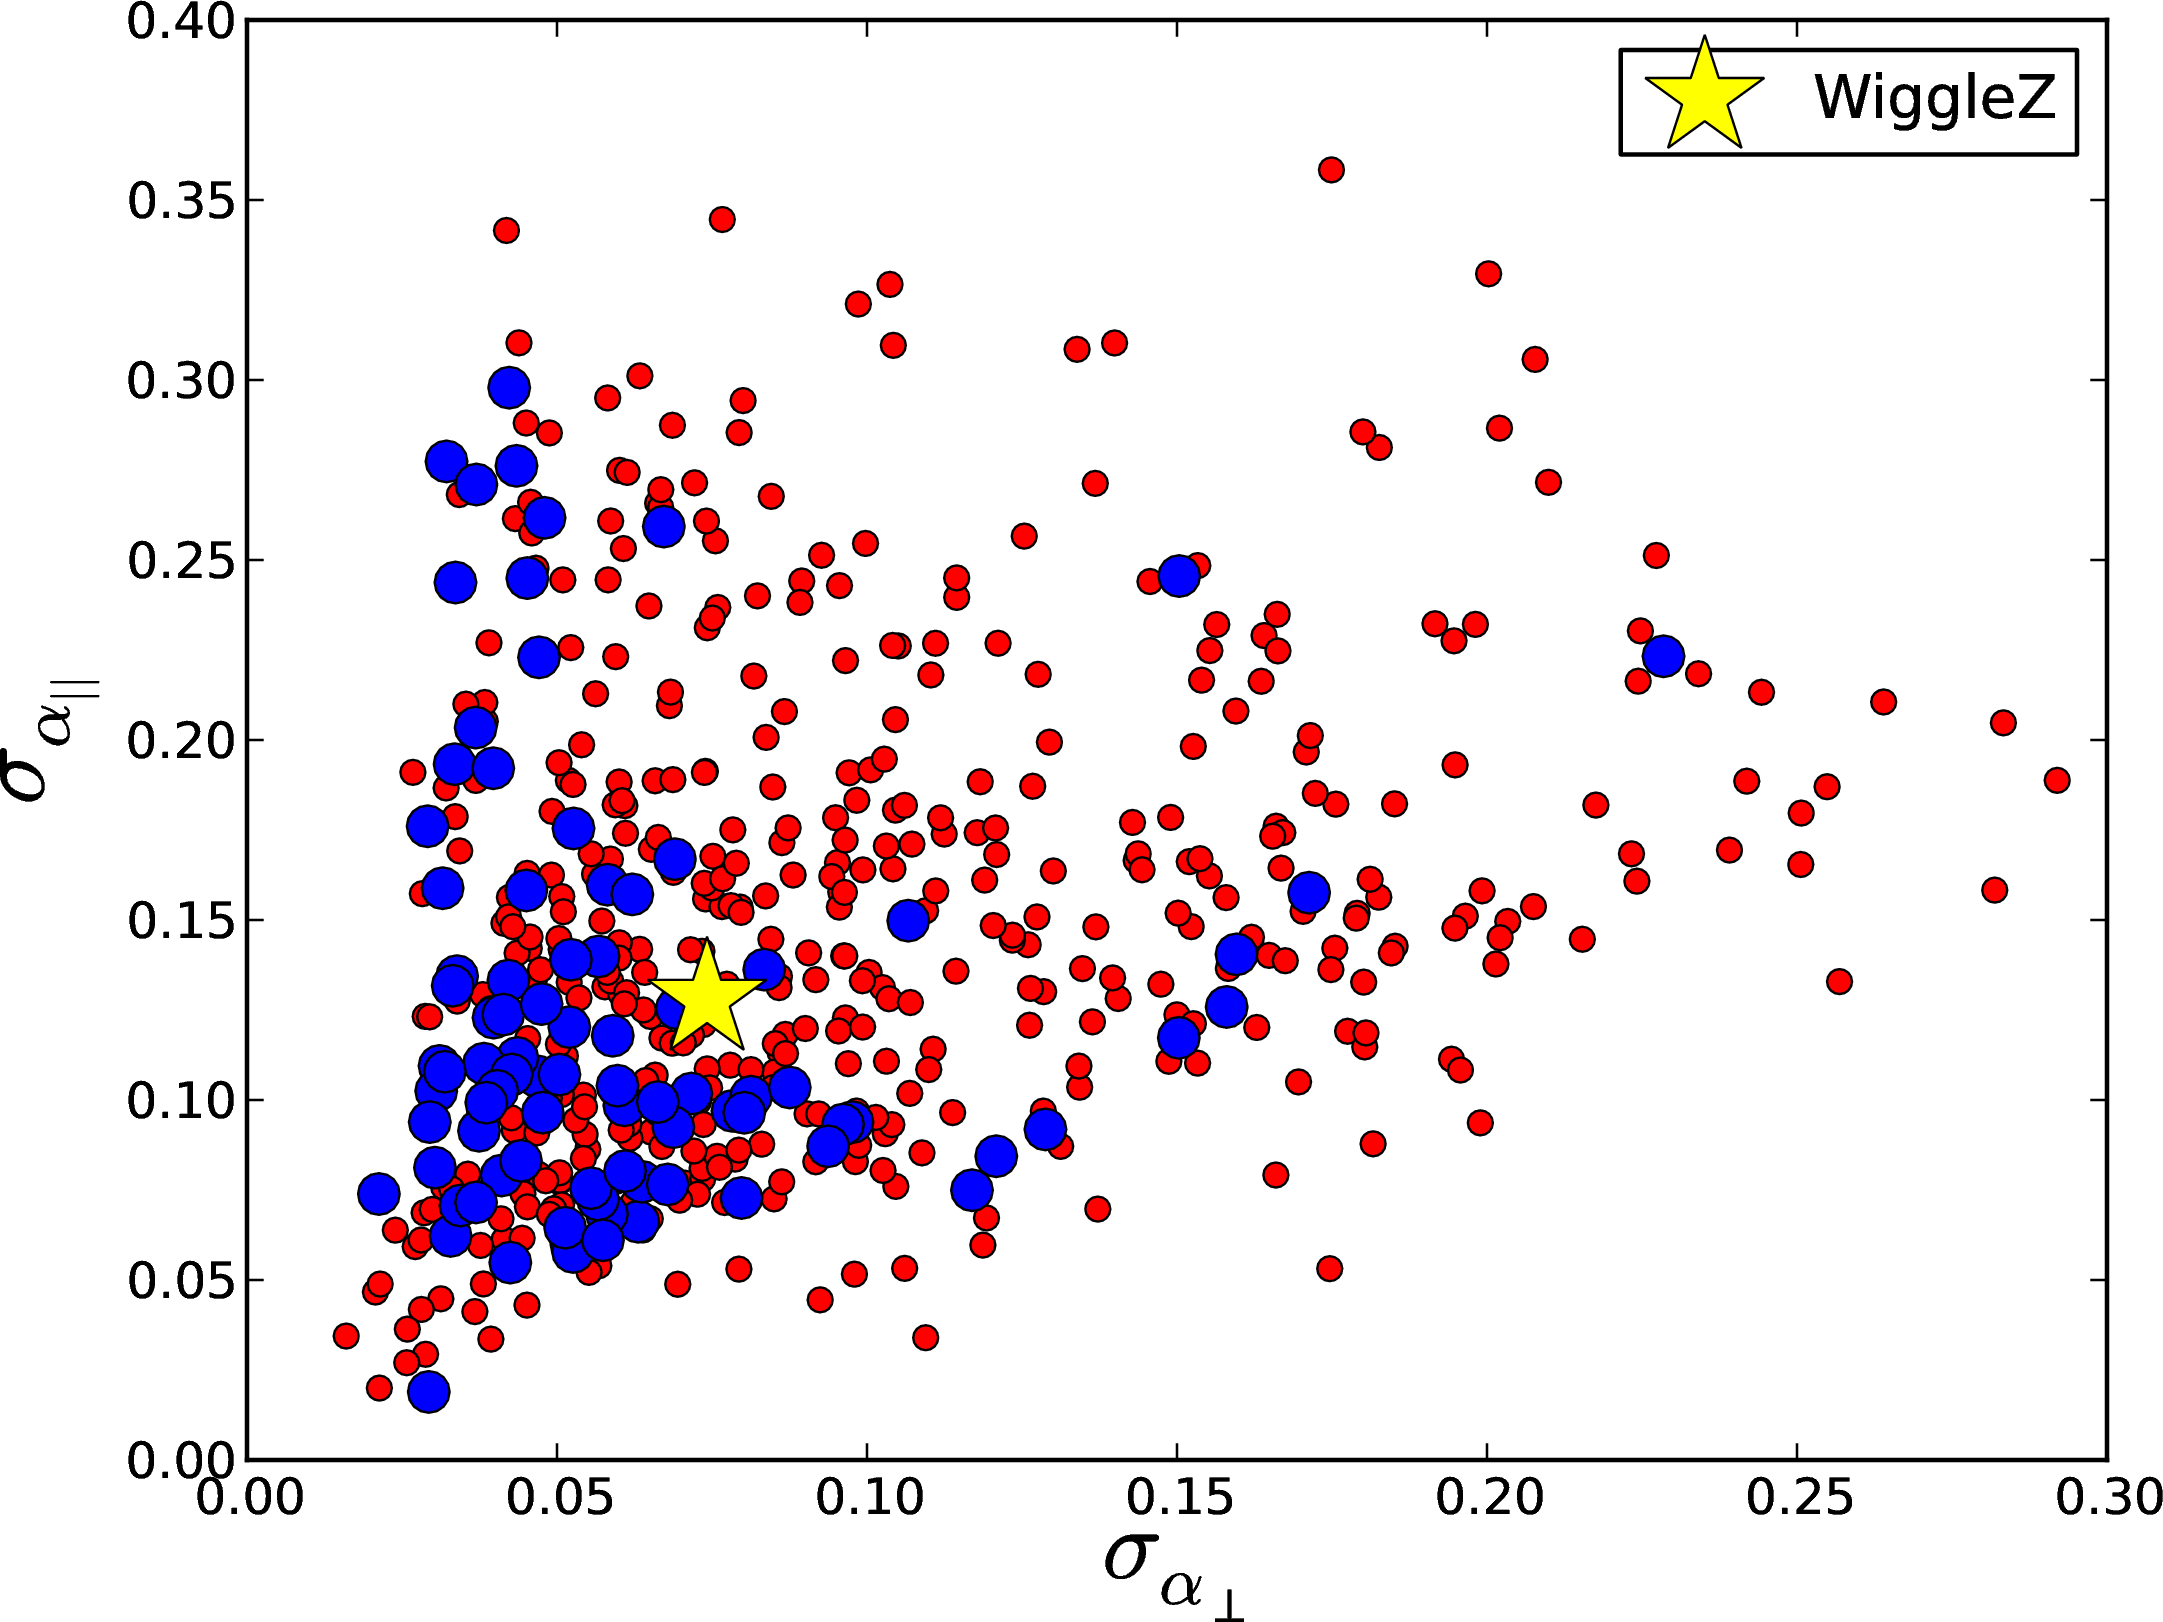
\includegraphics[width=0.7\columnwidth]{figures/WiZCOLA_unc_z0pt6_1pt0/WiZCOLA_unc_z0pt6_1pt0}
\caption{\label{fig:wizcola_hdaUnc_z60_epsilonT15} WiZCOLA $0.6<z<1$ $\alpha_{||}$ and $\alpha_\perp$ uncertainty results. The large blue circles are realizations that have a significance of detection of 2.9$\sigma$ (same as the observation) or higher. The red are below this threshold. For comparison, the star is the WiggleZ result.%
}
\end{center}
\end{figure}

\subsection{Combining redshift bins for reconstructed wedge data}
 {\blue
{\red [SAM Chris has a comment on this but I dont feel comfortably fleshing out that comment here without getting something wrong]}
**Describe how the correlation coefficients are derived, and how the correlation coefficients $(r)$ are derived in Table~\ref{tab:hda_wigglez_reconstructed}.**  **Why does Eyal say that the positive cross-correlation seen in the 0.44 bin is unphysical?**

} %END BLUE








\section{Unreconstructed Mulitpole Results}
\label{sec:multi}
{\blue Figure ** displays the multipole data .... (add figure and write something similar to what Eyal writes at the beginning of Section~\ref{sec:wedge}.  The could potentially be combined with Fig.~\ref{fig:wigglez_wedges_z60} but not necessarily. }

Using the methodology outlined in Sections~\ref{sec:test} we fit to the final unreconstructed WiggleZ dataset from \citet{KazinKoda2014} using both methods for combining redshift bins -- firstly fitting in each individual redshift bin and combining the results (Sect.~\ref{sec:parameterCov}), and secondly fitting all redshift bins simultaneously (Sect.~\ref{sec:allData}). The final distributions are given in Table \ref{tab:wigglezBinsParams} and illustrated in Figure~\ref{fig:wigglezBinsMP}.  The two methods give consistent results. 

%The wedge data analysis did not produce well behaved likelihood surfaces and cannot be used for analysis. This mirrors the issues found when attempting to constrain individual WizCOLA simulation realisations, and validates not utilising the wedge analysis.


The conversion from $\alpha$ and $\epsilon$ to $D_A(z)$ and $H(z) $ is given by equations \eqref{eq:alpha1} and \eqref{eq:alpha2}. Using these relationships, we formulate parameter constraints shown, also shown in Table \ref{tab:wigglezBinsParams}.

To determine the significance of the BAO peak detected in our analysis, we reran the multipole analysis with a model devoid of the BAO peak and converted the $\Delta \chi^2$ into a detection significance, which we found to be just over $2\sigma$ in all redshift bins. The low significance of the BAO peak is expected: the 1D BAO analysis from \citet{BlakeDavis2011} found a significance of $3.2\sigma$ when using all data in one combined bin, and as our analysis used the data divided over three bins, and includes extra parameters to model angular dependence, so it is expected the statistical significance of the BAO peak would decrease. The analysis in \citet{BlakeKazin2011}, which utilised three redshift bins, the same as our analysis, found statistical significances between $1.9\sigma$ and $2.4\sigma$, consistent with the results shown below.

%The final results for the WiggleZ 2D BAO cosmology analysis for the main parameters of interest are shown in {\red Table \ref{tab:wigglezBinsParams}. **COMBINE WITH TABLE~\ref{tab:wigglezBins}**}

\begin{figure}
	%\begin{wrapfigure}{r}{0.5\textwidth}
	\begin{center}
		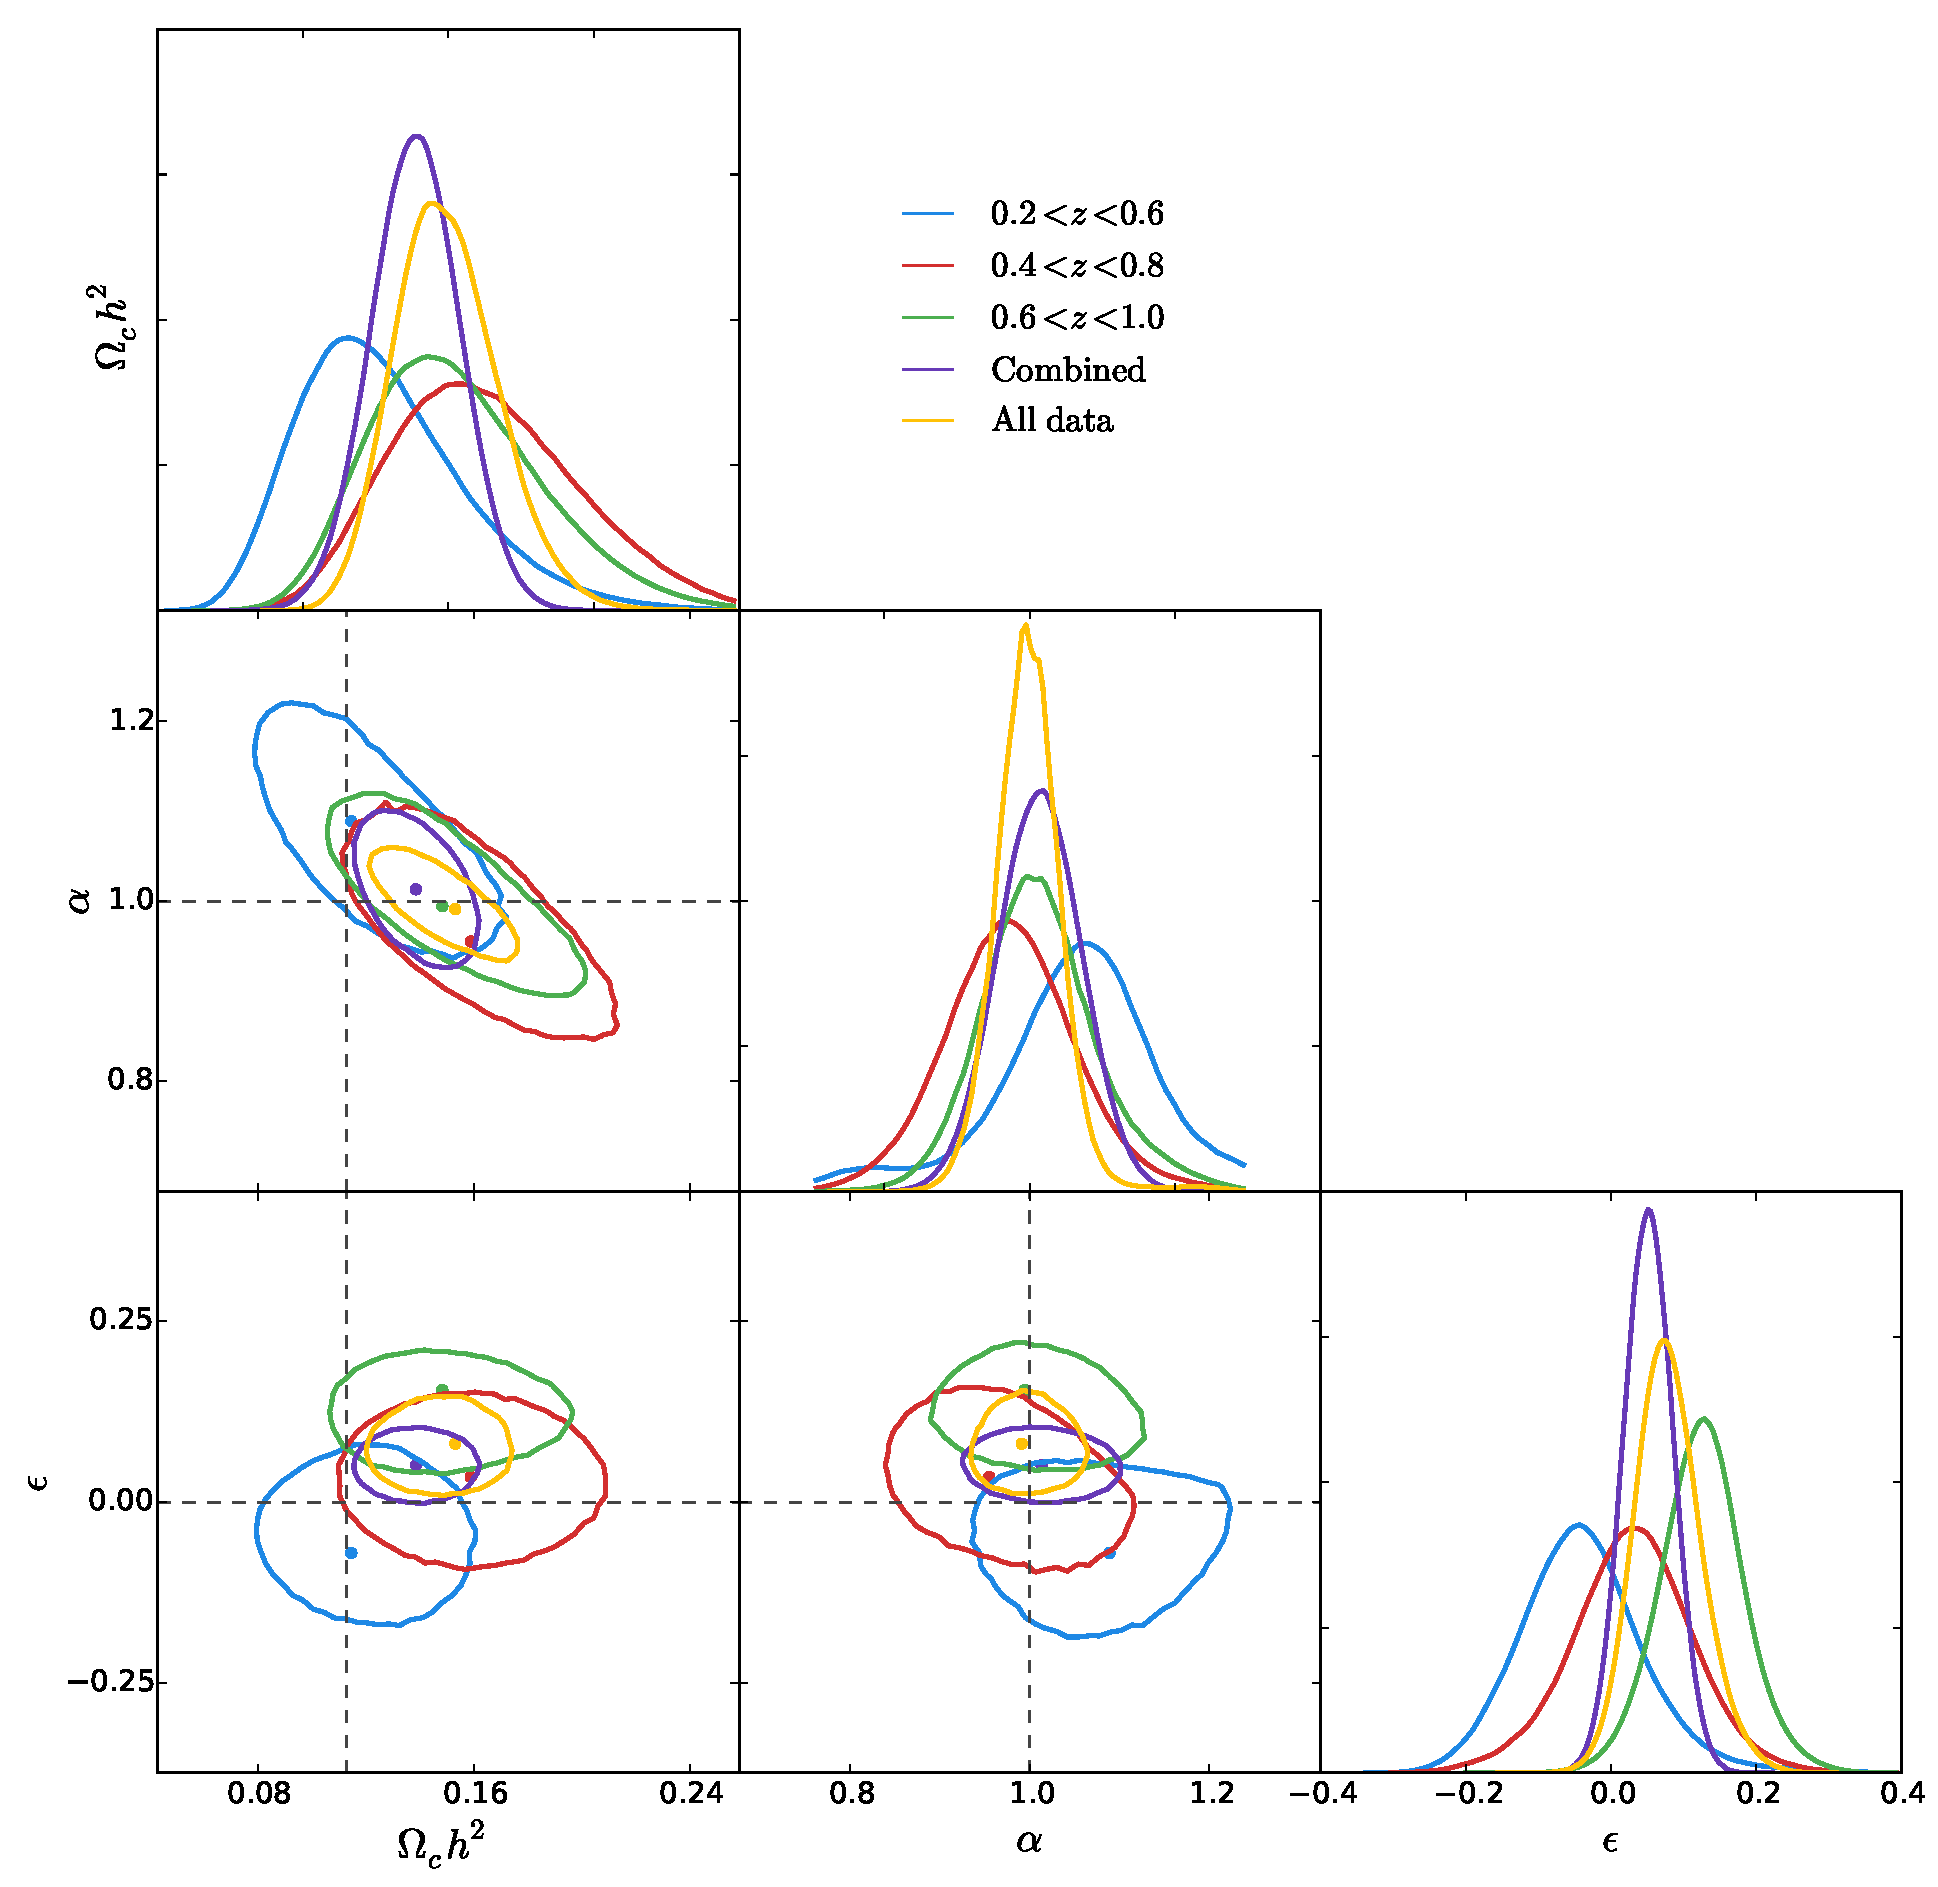
\includegraphics[width=\columnwidth]{images/corCombinedMPWig.pdf}
	\end{center}
	\caption{Likelihood surfaces and marginalised distributions of $\Omega_ch^2$, $\alpha$ and $\epsilon$ for the WiggleZ multipole expression of the data. }
	\label{fig:wigglezBinsMP}
	%\end{wrapfigure}
\end{figure}


\begin{table*}
	\centering
	\caption{Final parameter constraints from fitting the 2D BAO signal in the pre-reconstruction WiggleZ multipole correlation function.}
	%\resizebox{\textwidth}{!}{
	\begin{tabular}{cc|cc|ccc|ccc}
		\specialrule{.1em}{.05em}{.05em} 
		Sample & $z_{\rm{eff}}$ & $D^\prime_A(z)$ & $H^\prime(z)$ &  $\Omega_c h^2$  &$\alpha$ & $\epsilon$ & $D_A(z)$ & $H(z)$ & BAO peak significance\\
		\specialrule{.1em}{.05em}{.05em} 
		$0.2 < z < 0.6$ &  $0.44$ & 1175.5  & 87.4  & $0.117^{+0.029}_{-0.023}$ & $1.07^{+0.10}_{-0.10}$ & $-0.03^{+0.07}_{-0.10}$ & $1330 \pm  150$ & $85^{+19}_{-12}$  & $2.2\sigma$\\
		$0.4 < z < 0.8$ &  $0.6$  & 1386.2  & 95.5  & $0.156^{+0.035}_{-0.028}$ & $0.98^{+0.08}_{-0.10}$ & $0.05^{+0.07}_{-0.10}$ & $1280^{+190}_{-160}$ & $91^{+15}_{-14}$  & $2.1\sigma$\\
		$0.6 < z < 1.0$ &  $0.73$ & 1509.4  & 102.8 & $0.143^{+0.033}_{-0.026}$ & $1.00^{+0.08}_{-0.07}$ & $0.12^{+0.06}_{-0.05}$ & $1340^{+150}_{-130}$ & $80^{+9}_{-10}$  & $2.3\sigma$\\
		\specialrule{.1em}{.05em}{.05em} 
	\end{tabular}\label{tab:wigglezBinsParams}
	%}
\end{table*}





%\clearpage 
\begin{comment}
\begin{table}[]
\centering
\caption{}
\label{}
\begin{tabular}{cccc}
\hline
Model & $\Omega_c h^2$ & $D_A(z)$ & $H(z)$ \\ 
\hline
$0.2<z<0.6$ & $0.117^{+0.030}_{-0.023}$ & $1334.0^{+152.4}_{-153.6}$ & $85.0^{+18.5}_{-12.4}$ \\ 
$0.4<z<0.8$ & $0.156^{+0.033}_{-0.030}$ & $1281.1^{+192.1}_{-164.6}$ & $90.5^{+15.4}_{-13.6}$ \\ 
$0.6<z<1.0$ & $0.143^{+0.033}_{-0.026}$ & $1343.9^{+145.9}_{-134.9}$ & $80.4^{+9.1}_{-10.4}$ \\ 
\hline
\end{tabular}
\end{table}

\begin{table*}
	\centering
	\caption{{\red Combine with Table 5}  Recovered parameter constraints when fitting the WiggleZ multipole data. The $\chi^2$ column represents the minimum $\chi^2$ attained in the fit. The parameter values after combination are shown at the bottom of the table, where the $\chi^2$ value for the combined dataset indicates the $\chi^2$ from equation \eqref{eq:covchi} instead of the $\chi^2$ when fitting the cosmological model to the WiggleZ data. The effective redshift for the data in the ``All'' and ``Combined'' rows is $z=0.60$.}
%	\resizebox{\textwidth}{!}{
		\begin{tabular}{c|cccc}
			\specialrule{.1em}{.05em}{.05em} 
			$z_{\rm{eff}}$ & $\chi^2$ & $\Omega_c h^2$ &$\alpha$ & $\epsilon$ \\
			\specialrule{.1em}{.05em}{.05em} 
			$0.44$ & $51.8$ & $0.117^{+0.029}_{-0.023}$ & $1.07^{+0.10}_{-0.10}$ & $-0.03^{+0.07}_{-0.10}$  \\
			$0.60$ & $69.3$ & $0.154^{+0.035}_{-0.028}$ & $0.98^{+0.08}_{-0.10}$ & $0.05^{+0.07}_{-0.10}$   \\
			$0.73$ & $59.1$ & $0.144^{+0.033}_{-0.026}$ & $1.00^{+0.08}_{-0.07}$ & $0.12^{+0.06}_{-0.05}$ \\
			\specialrule{.05em}{.05em}{.05em} 
			All & $255.0$   & $0.147^{+0.018}_{-0.018}$ & $1.00^{+0.05}_{-0.04}$ & $0.08^{+0.04}_{-0.05}$   \\
			\specialrule{.05em}{.05em}{.05em} 
			Combined & $5.6$ & $0.140^{+0.014}_{-0.017}$ & $1.00^{+0.07}_{-0.05}$ & $0.06^{+0.03}_{-0.04}$  \\
			\specialrule{.1em}{.05em}{.05em} 
		\end{tabular}\label{tab:wigglezBins}
%	}
\end{table*}



\begin{table*}
	\centering
	\caption{Final parameter constraints from fitting the 2D BAO signal in the WiggleZ multipole correlation function. {\red **Report our results without the $r_s$? And combine with Table~\ref{tab:wigglezBins} and Table~\ref{tab:hda_wigglez_reconstructed}?**}}
	%\resizebox{\textwidth}{!}{
		\begin{tabular}{cc|cc|cccc}
			\specialrule{.1em}{.05em}{.05em} 
			Sample & $z_{\rm{eff}}$ & $D^\prime_A(z)$ & $H^\prime(z)$ &  $\Omega_c h^2$   & $D_A(z)/r_s$ & $cz/H(z)/r_s $ & BAO peak significance\\
			\specialrule{.1em}{.05em}{.05em} 
			$0.2 < z < 0.6$ &  $0.44$ & 1175.5  & 87.4  & $0.117^{+0.029}_{-0.023}$ & $8.76^{+0.98}_{-1.02}$ & $9.5^{+1.7}_{-1.6}$  & $2.2\sigma$\\
			$0.4 < z < 0.8$ &  $0.6$  & 1386.2  & 95.5  & $0.154^{+0.035}_{-0.028}$ & $8.3^{+1.3}_{-1.0}$ & $12.7^{+1.9}_{-2.1}$  & $2.1\sigma$\\
			$0.6 < z < 1.0$ &  $0.73$ & 1509.4  & 102.8 & $0.144^{+0.033}_{-0.026}$ & $8.81^{+0.95}_{-0.89}$ & $17.7^{+2.2}_{-2.1}$  & $2.3\sigma$\\
			\specialrule{.1em}{.05em}{.05em} 
		\end{tabular}\label{tab:wigglezBinsParams2}
	%}
\end{table*}

\end{comment}




%============================================================
\begin{table*}
\begin{centering}
\caption{Model-independent measurements using the post-reconstruction $\xi_{||,\perp}$.}
\label{tab:hda_wigglez_reconstructed}
\begin{tabular}{ l | r | r | c | c | c | c | r }
\hline
              & \multicolumn{2}{c}{Fiducial} & \multicolumn{5}{c}{Measured} \\  
              &  & & Measured & & & & \\
$z_{\rm eff}$ & $cz/H/r_{\rm s}$ & $D_{\rm A}/r_{\rm s}$  & $cz/H/r_{\rm s}$ & $D_{\rm A}/r_{\rm s}$  & $r$ & $\chi^2$ & $\Delta\chi^2$ \\
\hline
  0.73  & 13.87 & 9.84 & 15.3$^{+2.1}_{-1.8}$ (13\%)  &  9.8$^{+1.1}_{-0.4}$ (7\%)   & -0.36  & 35 & 8.4 \\
  0.60  & 12.27 & 9.03 & 11.5$^{+1.3}_{-1.6}$ (13\%)  & 10.3$^{+0.4}_{-0.5}$ (5\%)   & -0.16  & 25 & 7.2 \\
%  0.44  &  9.84 & 8.87 &  7.4$^{+4.5}_{-0.2}$ (32\%)  &  8.7$^{+1.0}_{-2.6}$ (21\%)  & +0.44  & 35 & 2.5 \\
%----------
%$z_{\rm eff}$ & $cz/H/r_{\rm s}$ & $D_{\rm A}/r_{\rm s}$  & $r$ & $\chi^2$ & $\Delta\chi^2$ \\
%\hline
%  0.73  & 15.30$^{+2.11}_{-1.8}$ (12.8\%)  & 9.79$^{+1.09}_{-0.36}$ (7.4\%)   & -0.36  & 34.4 & 8.4 \\
%  0.60   & 11.50$^{+1.31}_{-1.63}$ (12.8\%) & 10.33$^{+0.43}_{-0.54}$ (4.7\%)  & -0.16  & 24.8 & 7.2 \\
%  0.44  & 7.40$^{+4.50}_{-0.2}$ (31.8\%)   & 8.72$^{+0.97}_{-2.63}$ (20.6\%)  & +0.44 & 35.3 & 2.5 \\
\end{tabular}

\medskip
The values quoted are the modes and the $68\%$ CL regions. The percentages indicate half of the $68\%$ CL regions. \\
%Fiducial values for $cz/H/r_{\rm s}$ used ($z=0.73,\ 0.6, \ 0.44$, respectively): 13.87, 12.27, 9.84. \\
%Fiducial values for $D_{\rm A}/r_{\rm s}$ used ($z=0.73,\ 0.6, \ 0.44$, respectively): 9.84, 9.03, 8.87.\\
Fiducial values for $cz/H/r_{\rm s}$ used ($z=0.73,\ 0.6$, respectively): 13.87, 12.27. \\
Fiducial values for $D_{\rm A}/r_{\rm s}$ used ($z=0.73,\ 0.6$, respectively): 9.84, 9.03.\\
%{\red The positive cross-correlation $r$ for the $z_{\rm eff}=0.44$ is not physical, but rather due to the flat priors used. **WHY?**} \\
Values for the $z=0.44$ bin are not report as the data was insufficient to provide constraints and final surfaces were heavily dependent on choice of prior.
In the $\chi^2$ fitting we use 36 dof. \\
$\Delta\chi^2\equiv \chi^2_{\rm no-wiggle} - \chi^2_{\rm \Lambda CDM-based}$. \\
These results are displayed in Figure \ref{fig:hubble_diagram}. \\
\end{centering}
\end{table*}
%============================================================

%\clearpage


\section{Reconstructed Results}\label{sec:wedge}

Figure \ref{fig:wigglez_wedges_z60} displays the clustering wedges
$\xi_\perp(s)$ (transverse wedge $\mu<0.5$; blue squares) and
$\xi_\parallel(s)$ (line-of-sight wedge $\mu>0.5$; red circles) in the
three redshift ranges investigated $\Delta z^{\rm Near}$, $\Delta
z^{\rm Mid}$ and $\Delta z^{\rm Far}$.  We overplot best-fitting
models for which we calculated $\chi^2 = 35.3, 24.8$ and $34.4$,
respectively, with 36 degrees of freedom.  We see baryonic acoustic
peak signatures in both $\xi_\perp$ and $\xi_\parallel$ for all three
redshift ranges.  The fluctuations from zero at large scales are
consistent with the characteristic sample variance seen in the WiZCOLA
simulations.

Figure \ref{fig:HDA_z26_epsilon0.15} displays the posterior
probability distributions of $cz/H/r_{\rm s}$ and $D_{\rm A}/r_{\rm
  s}$. In the 2D panels the solid red contours indicate $68\%$ and
$95\%$ confidence level regions, and we indicate a Gaussian
approximation in each panel based on the statistics of the full
probability distributions.  It is apparent that the BAO-only analysis
of the $\Delta z^{\rm Far}$ and $\Delta z^{\rm Mid}$ samples yield
reasonable distance constraints, whereas the data in the $\Delta
z^{\rm Near}$ bin lacks the constraining power needed to draw
significant conclusions.  Table~\ref{tab:hda_wigglez_reconstructed} lists our resulting measurements of
$D_{\rm A}/r_{\rm s}$ and $1/H/r_{\rm s}$.

To quantify the significance of detection of the anisotropic baryonic
feature in the WiggleZ clustering wedges we compared $\chi^2$ results
obtained with best-fit models using a $\Lambda$CDM-based template and
a ``no-wiggles'' template ($\Delta\chi^2 \equiv \chi^2_{\rm min,
  no-wiggle} - \chi^2_{\rm min, \Lambda CDM}$).  In this procedure,
for each model we vary $H r_{\rm s}$ and $D_{\rm A}/r_{\rm s}$ and
marginalize over all other shape parameters, as explained in detail in
\S 6.1 of \citet{KazinSanchezCuesta2013}.  We find that the significance of
detection, defined as $\sqrt{\Delta\chi^2}$ to be $1.6$, $2.7$ and
$2.9$ for $\Delta z^{\rm Near}$, $\Delta z^{\rm Mid}$ and $\Delta
z^{\rm Far}$, respectively.  Applying our pipeline to the WiZCOLA
simulations, we find our results are consistent with the range of
expectations.




\begin{figure}[!h]
\begin{center}
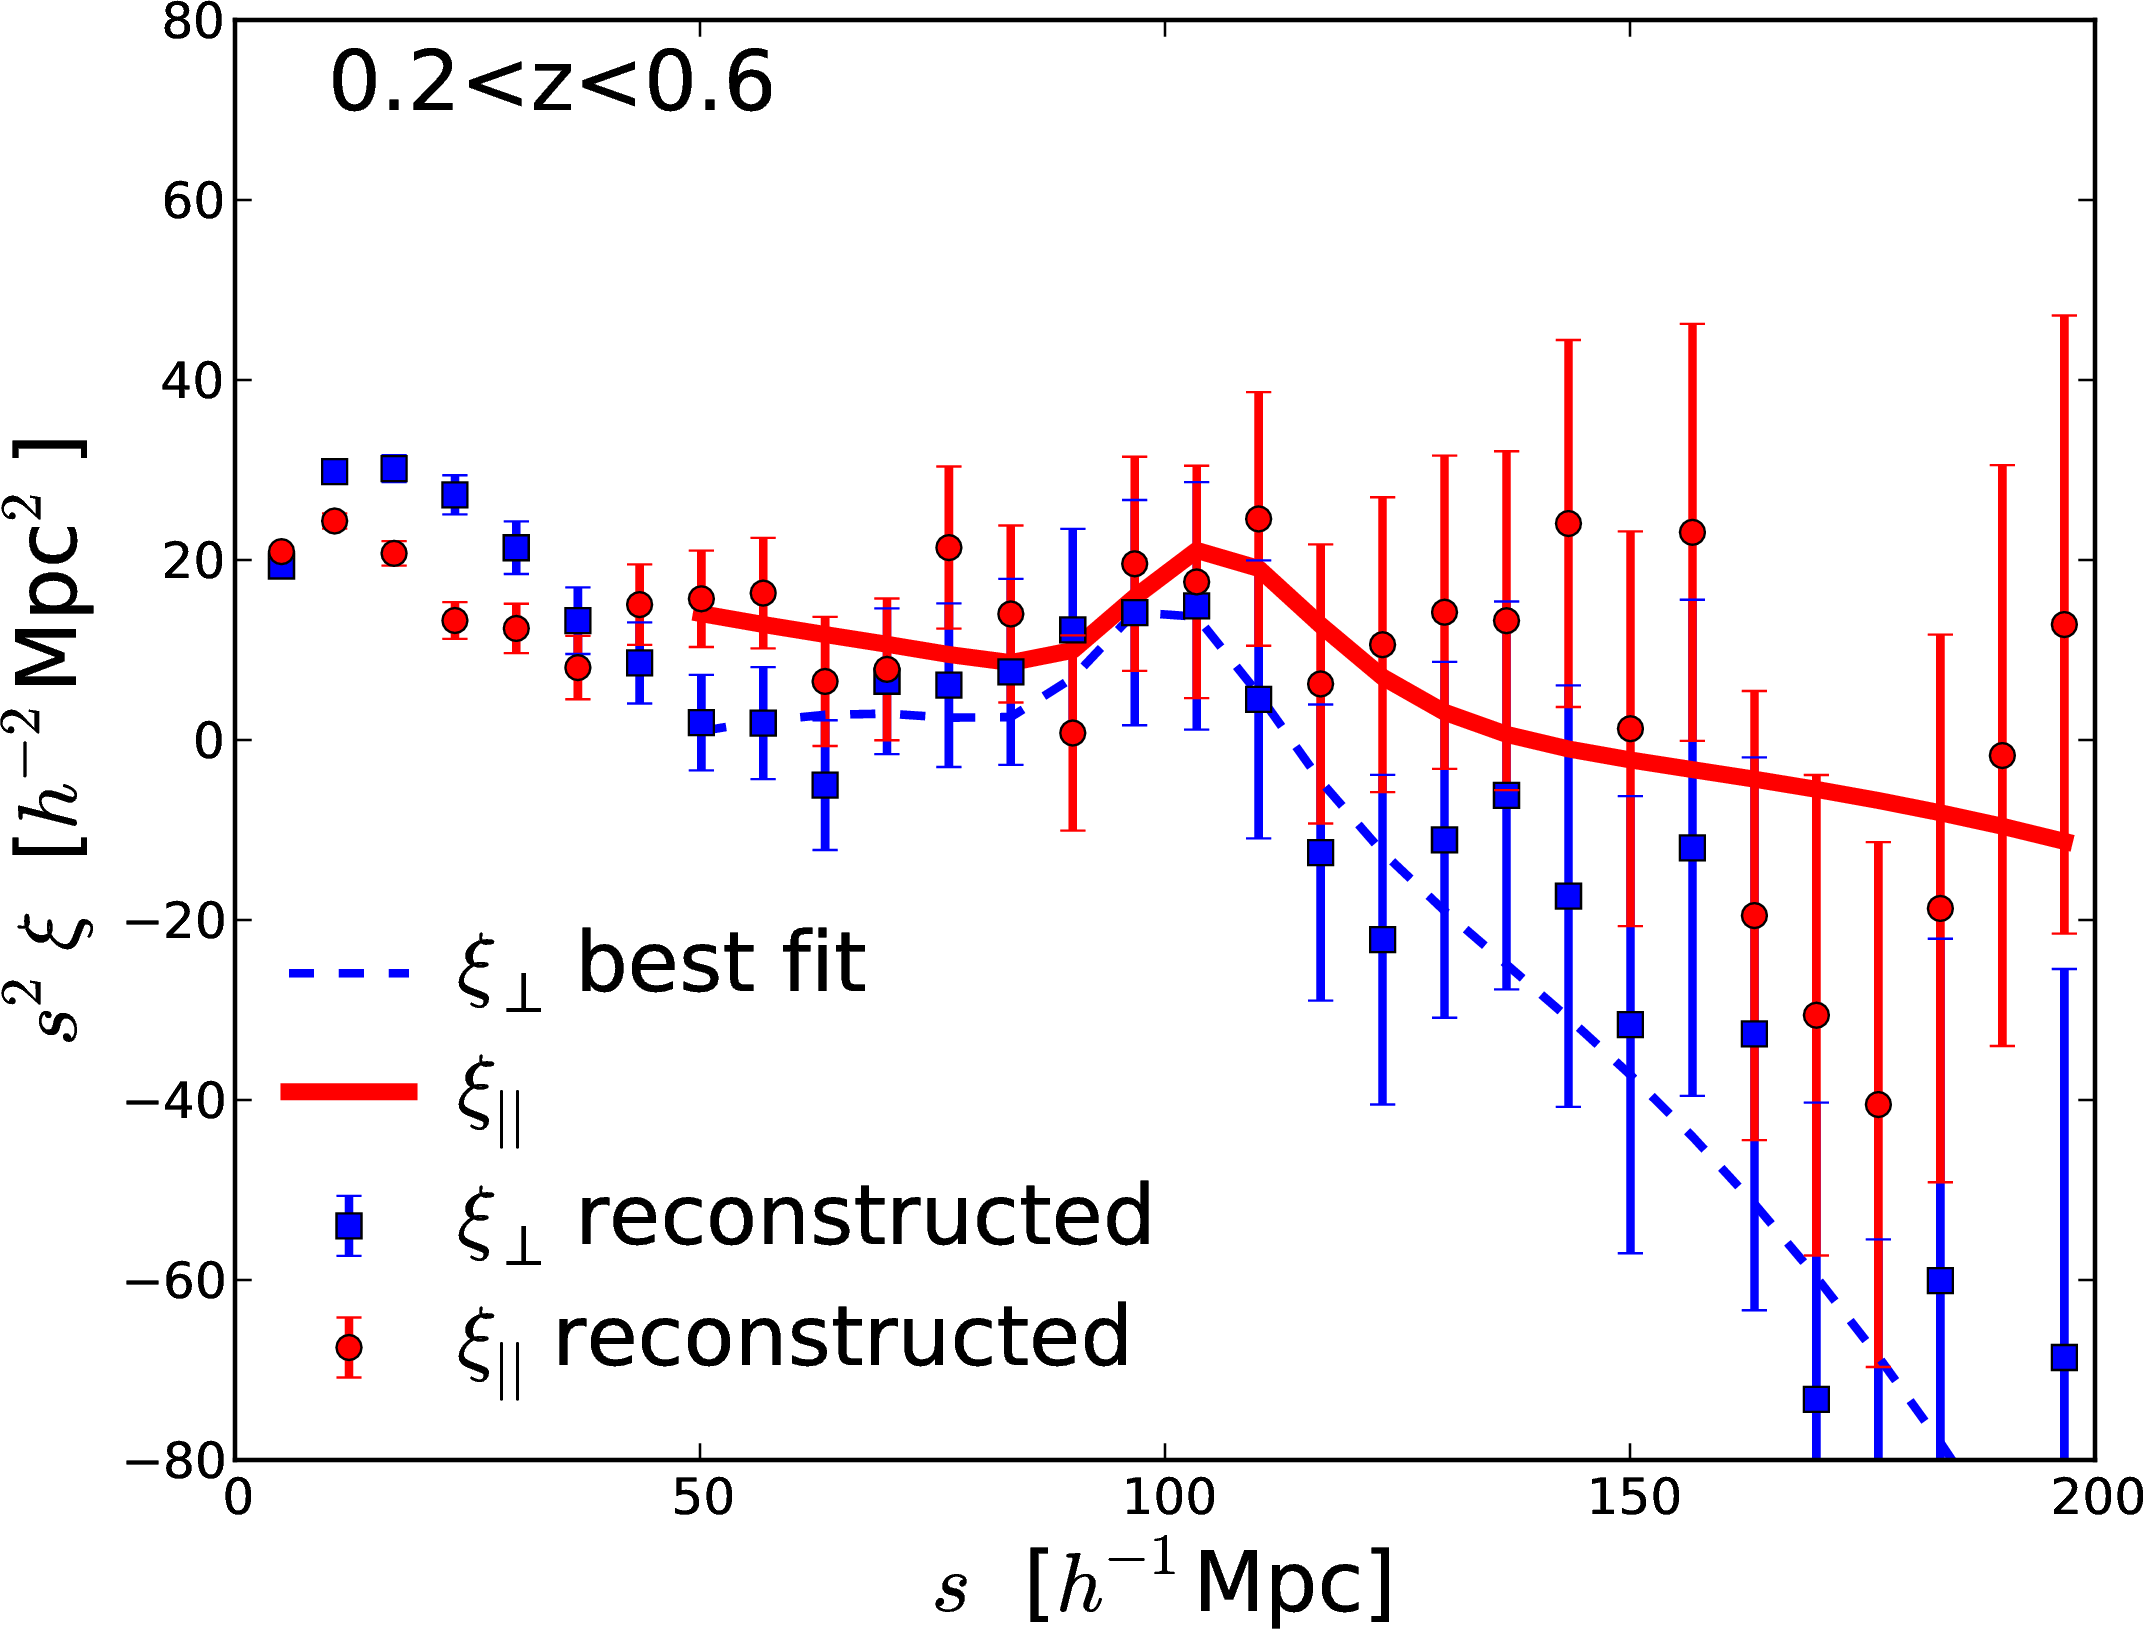
\includegraphics[width=0.9\columnwidth]{figures/WiggleZ_post_rec_Xiwedges_z26/WiggleZ_pre_post_rec_Xiwedges_z26}
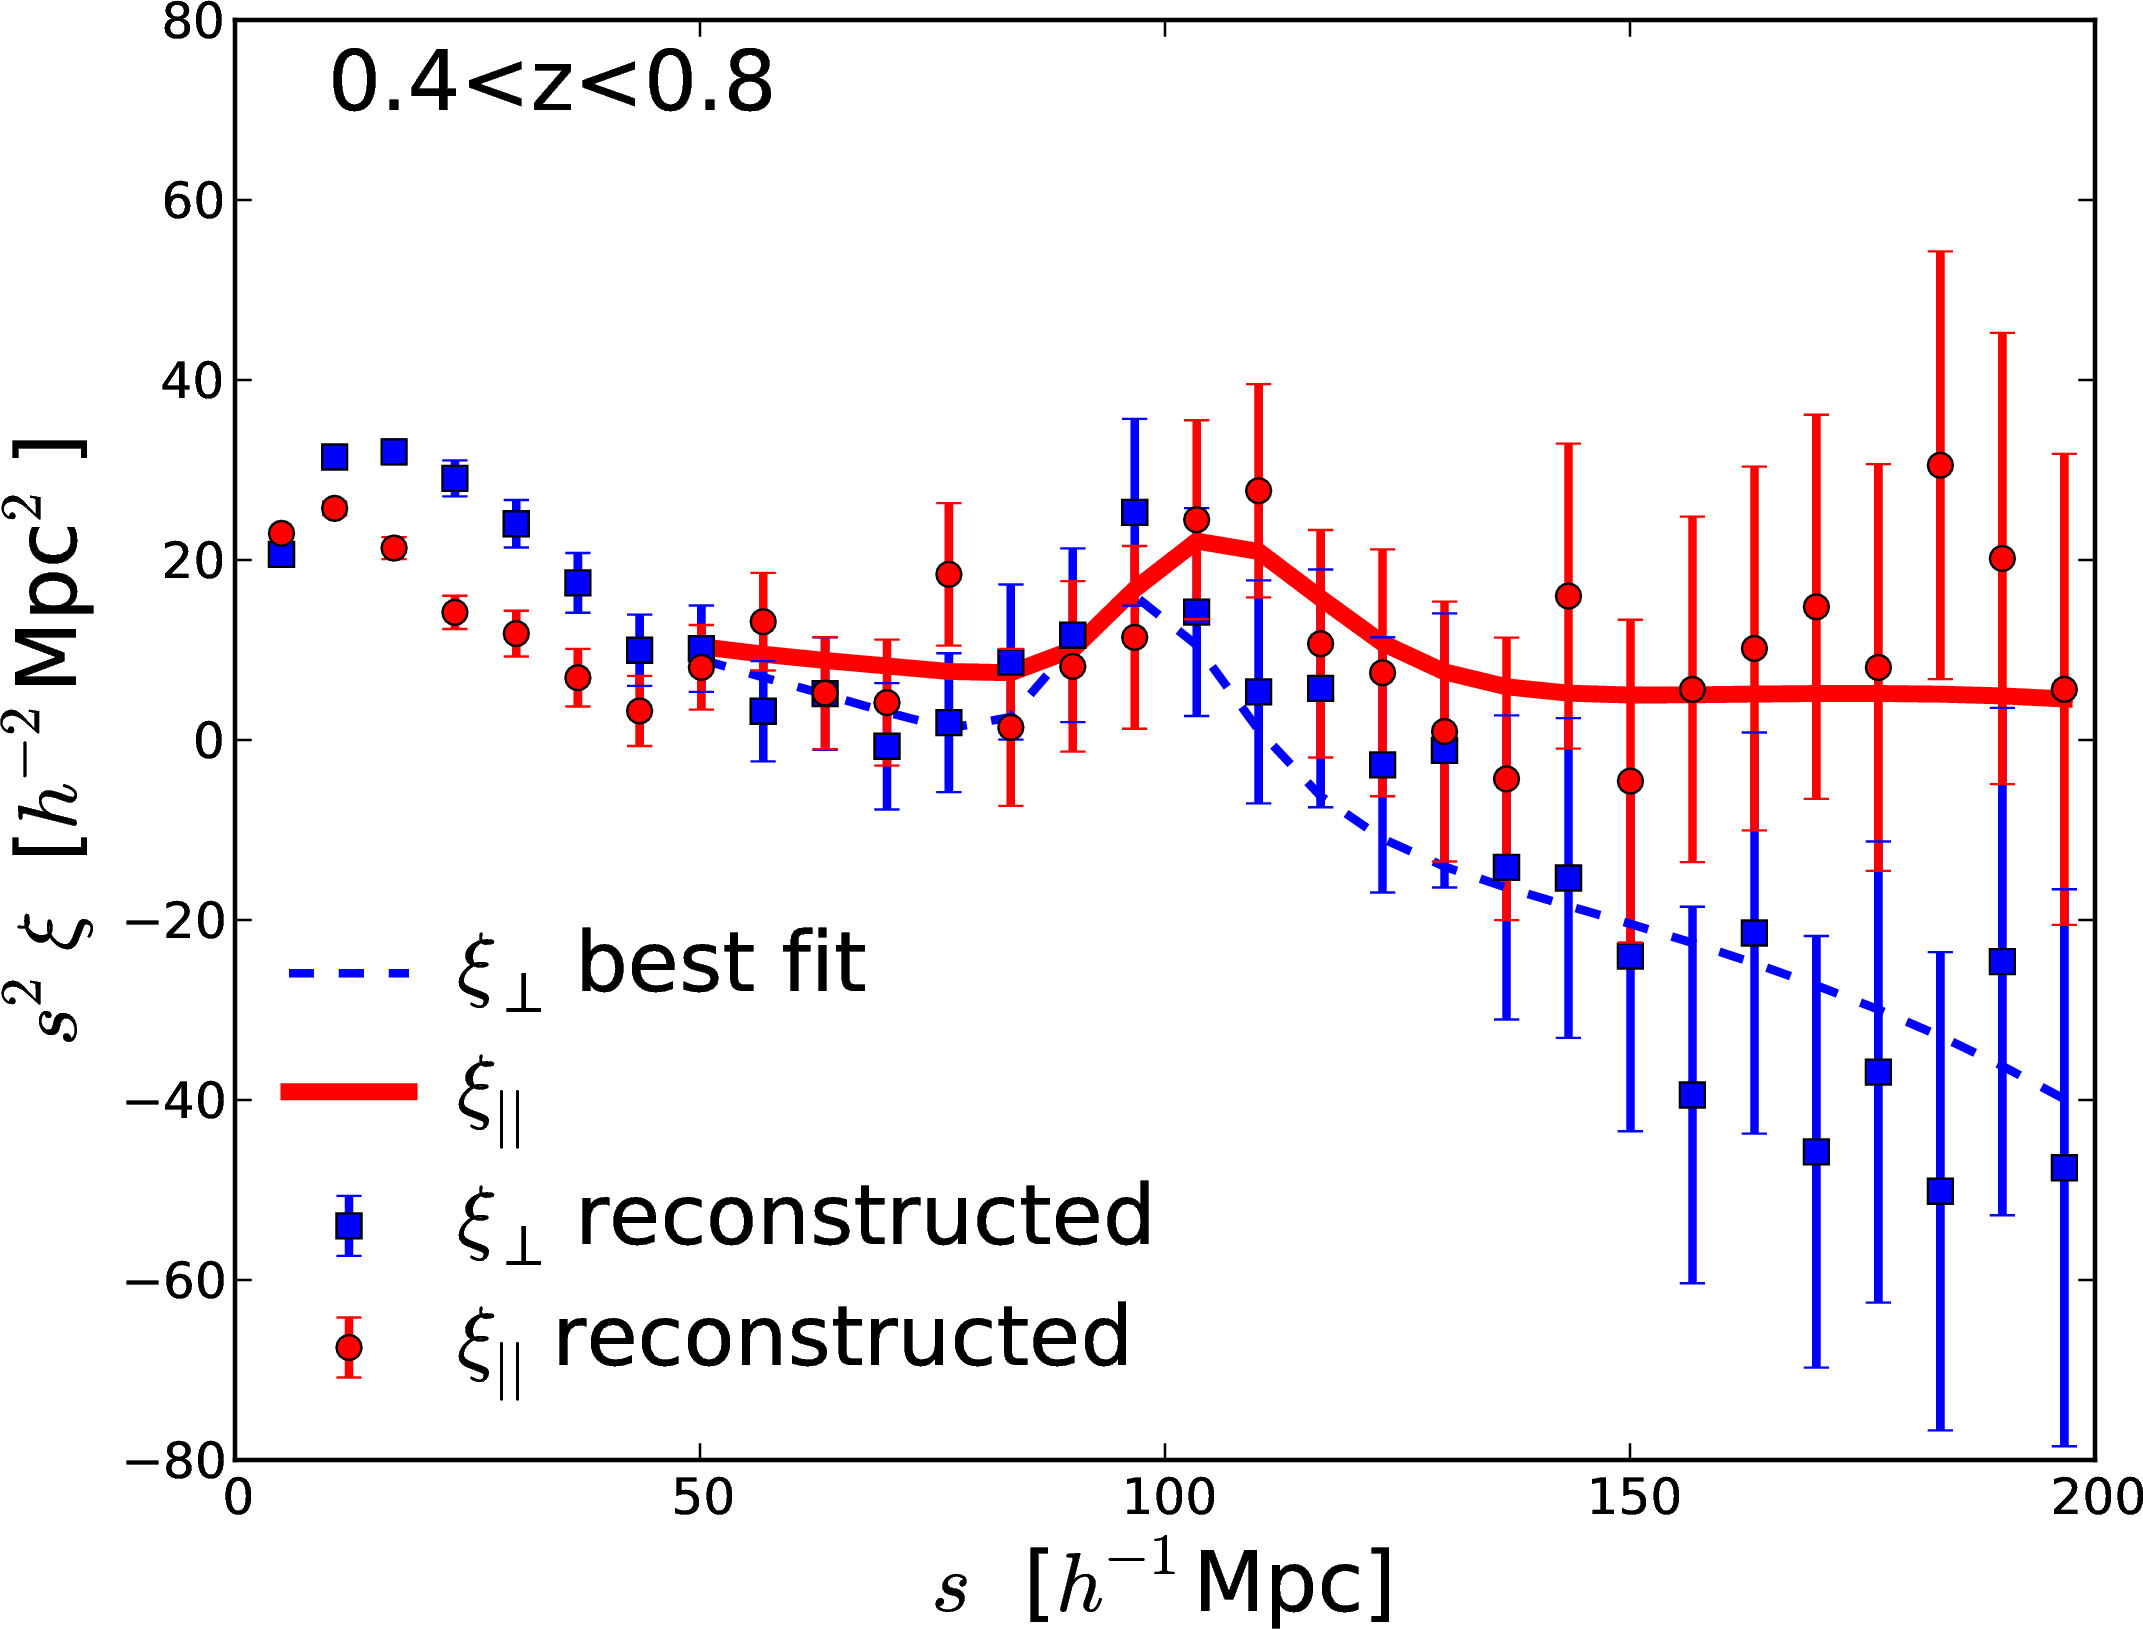
\includegraphics[width=0.9\columnwidth]{figures/WiggleZ_post_rec_Xiwedges_z48/WiggleZ_pre_post_rec_Xiwedges_z48}
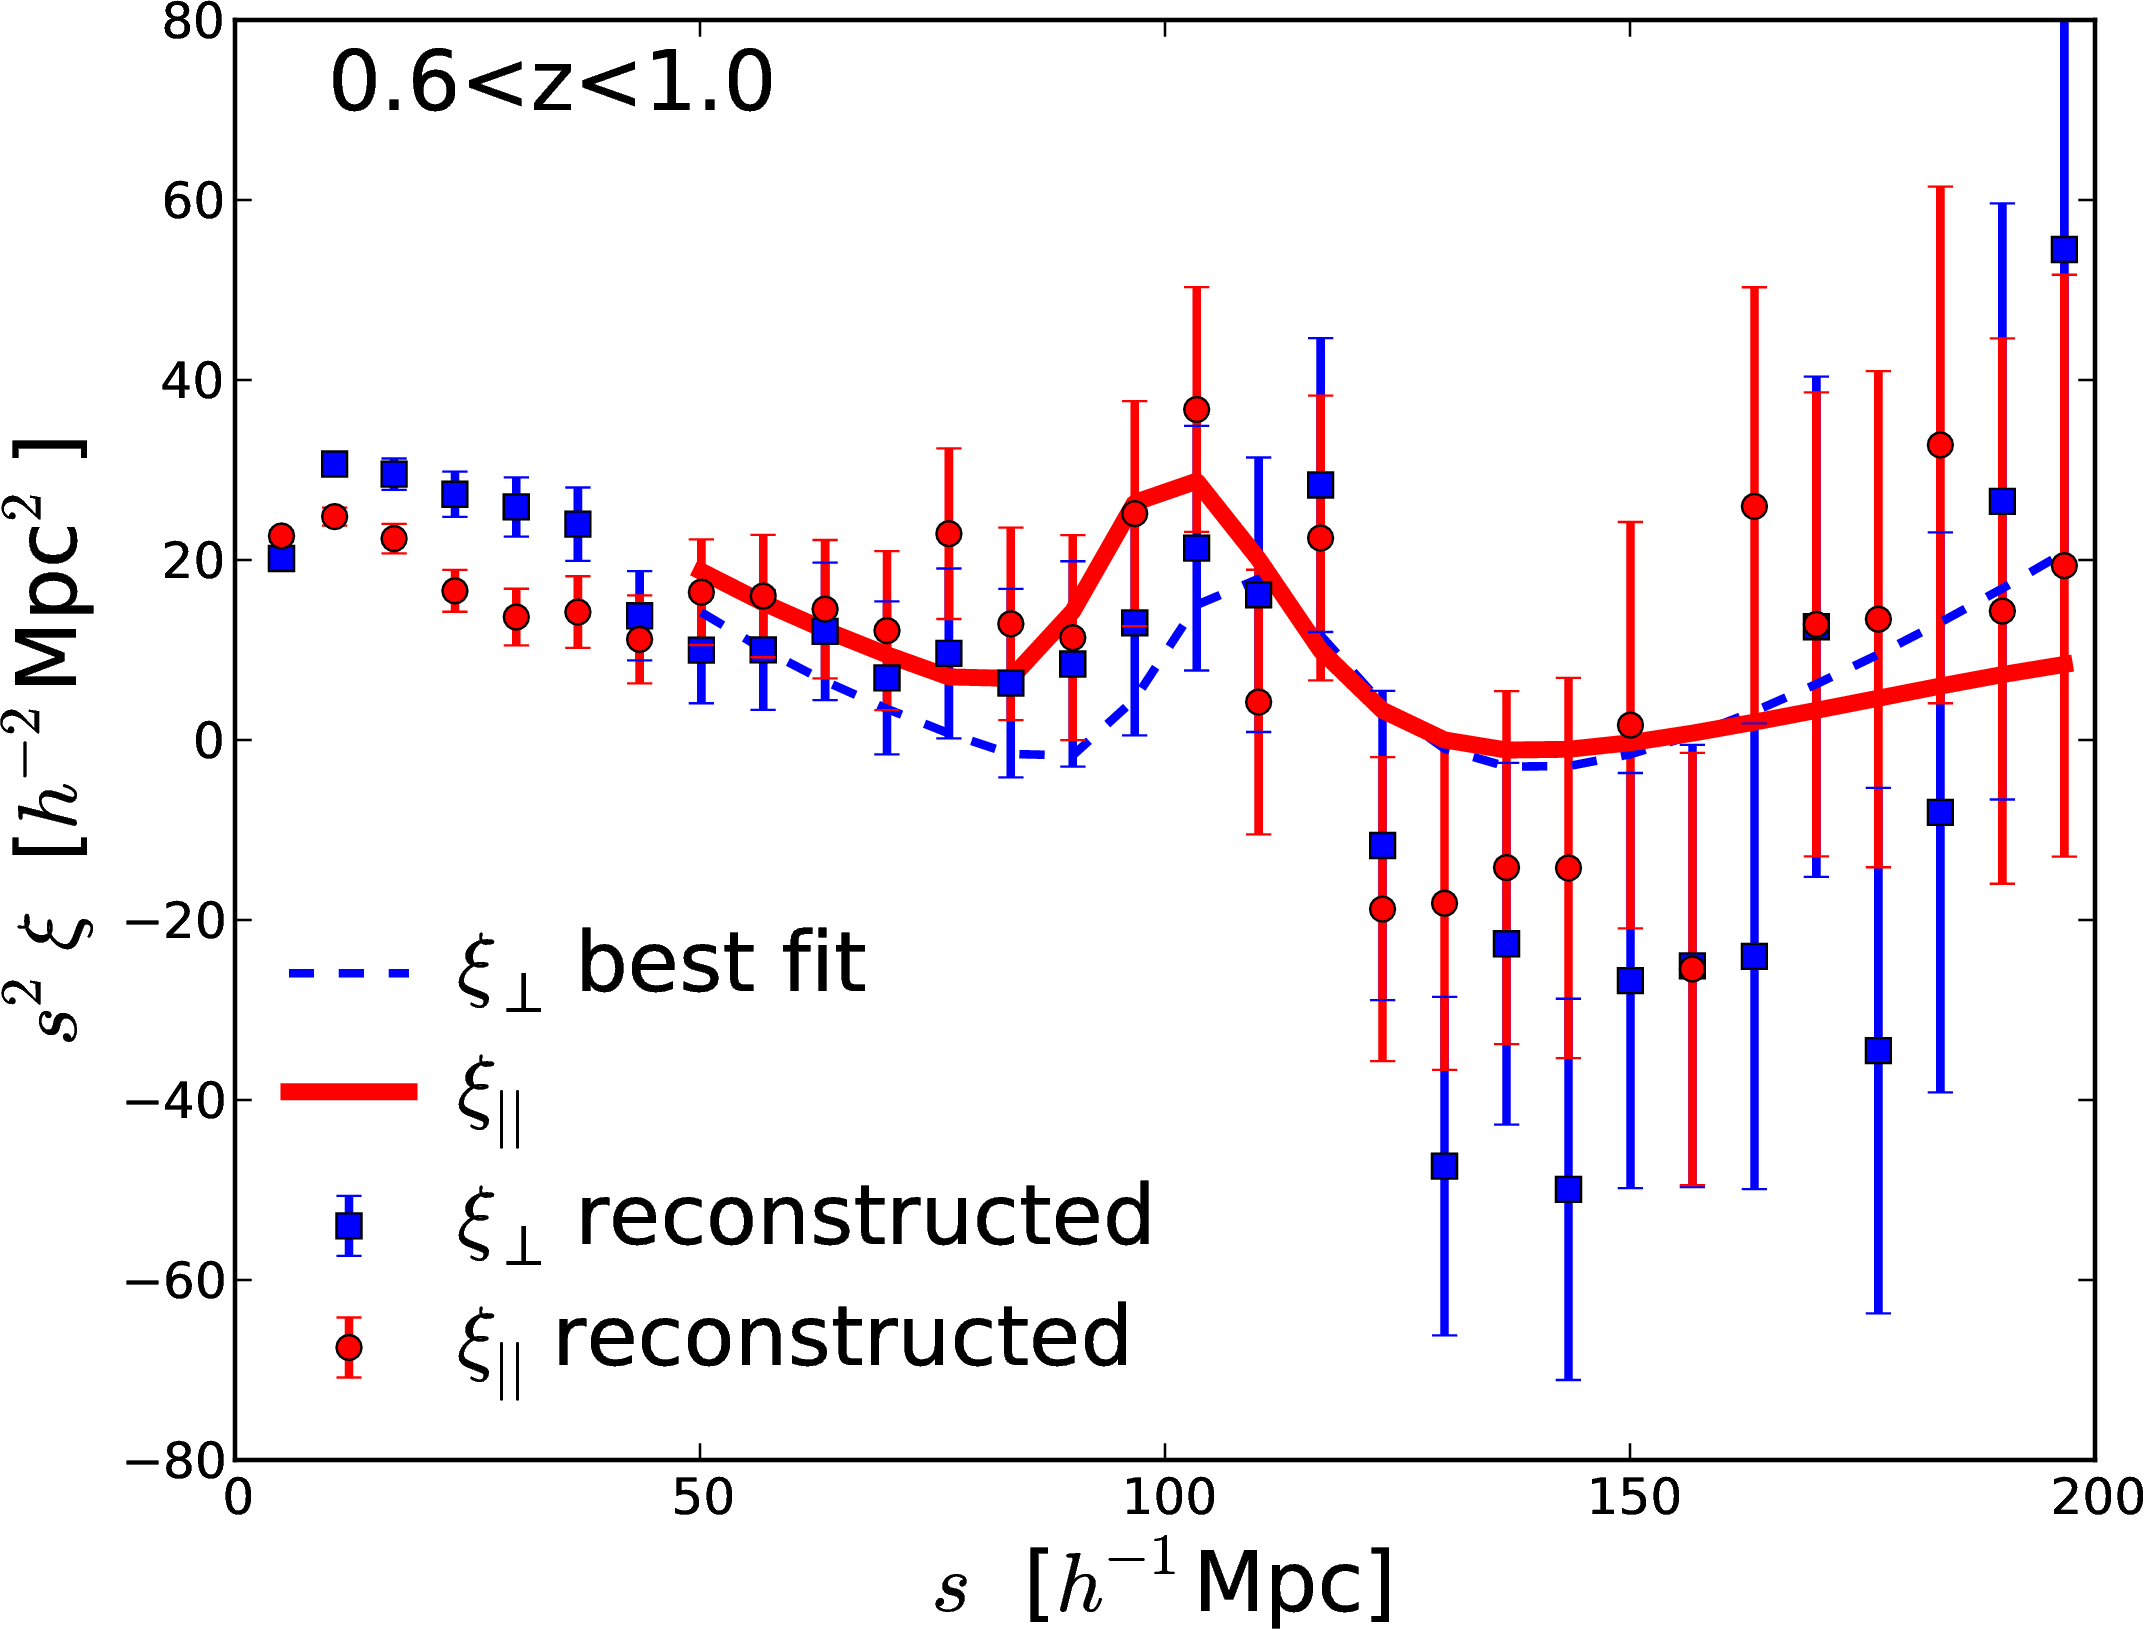
\includegraphics[width=0.9\columnwidth]{figures/WiggleZ_post_rec_Xiwedges_z60/WiggleZ_pre_post_rec_Xiwedges_z60}
\caption{\label{fig:wigglez_wedges_z60}  {\red ADD MULITPOLE DATA} WiggleZ post-reconstruction $0.2<z<0.6$ (upper), $0.4<z<0.8$ (mid), $0.6<z<1$ (lower) clustering $\xi_{||}$ (red line-of-sight; red circles), $\xi_{\perp}$ (transverse; blue squares) and best-fit models.%
}
\end{center}
\end{figure}


\begin{figure}
\begin{center}
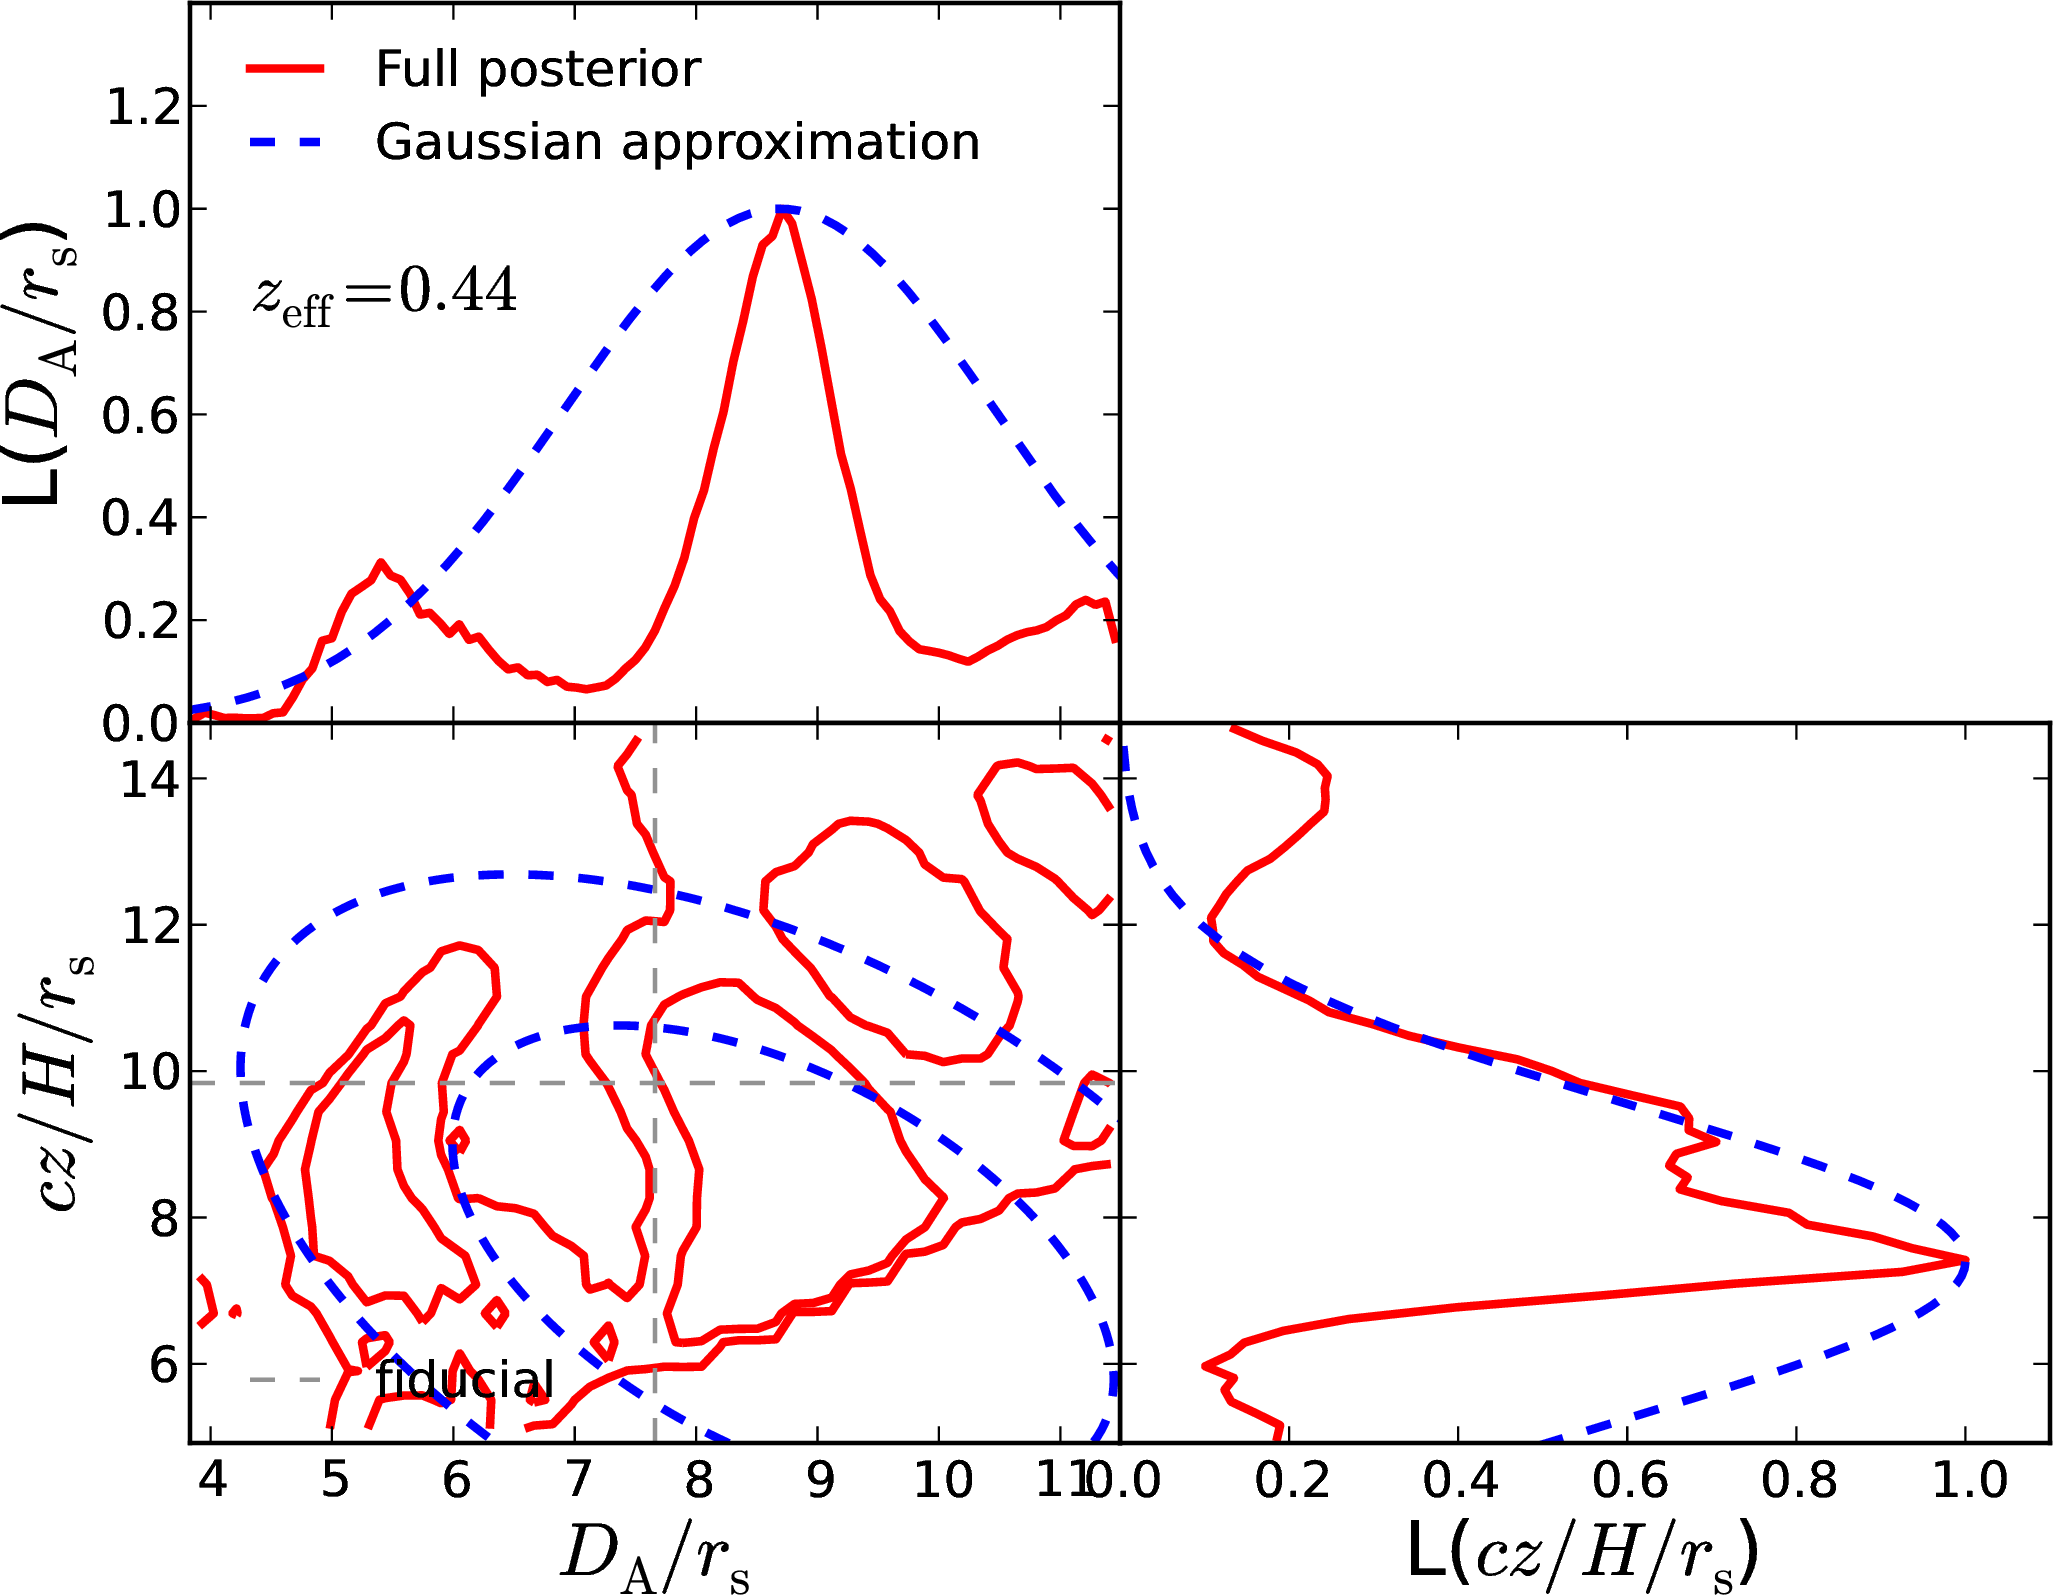
\includegraphics[width=0.9\columnwidth]{figures/stacked_L2D_rpt_wedges_postRec_T0.15_WiggleZ_z0pt2_0pt1/stacked_L2D_rpt_wedges_postRec_T015_WiggleZ_z0pt2_0pt6.png}
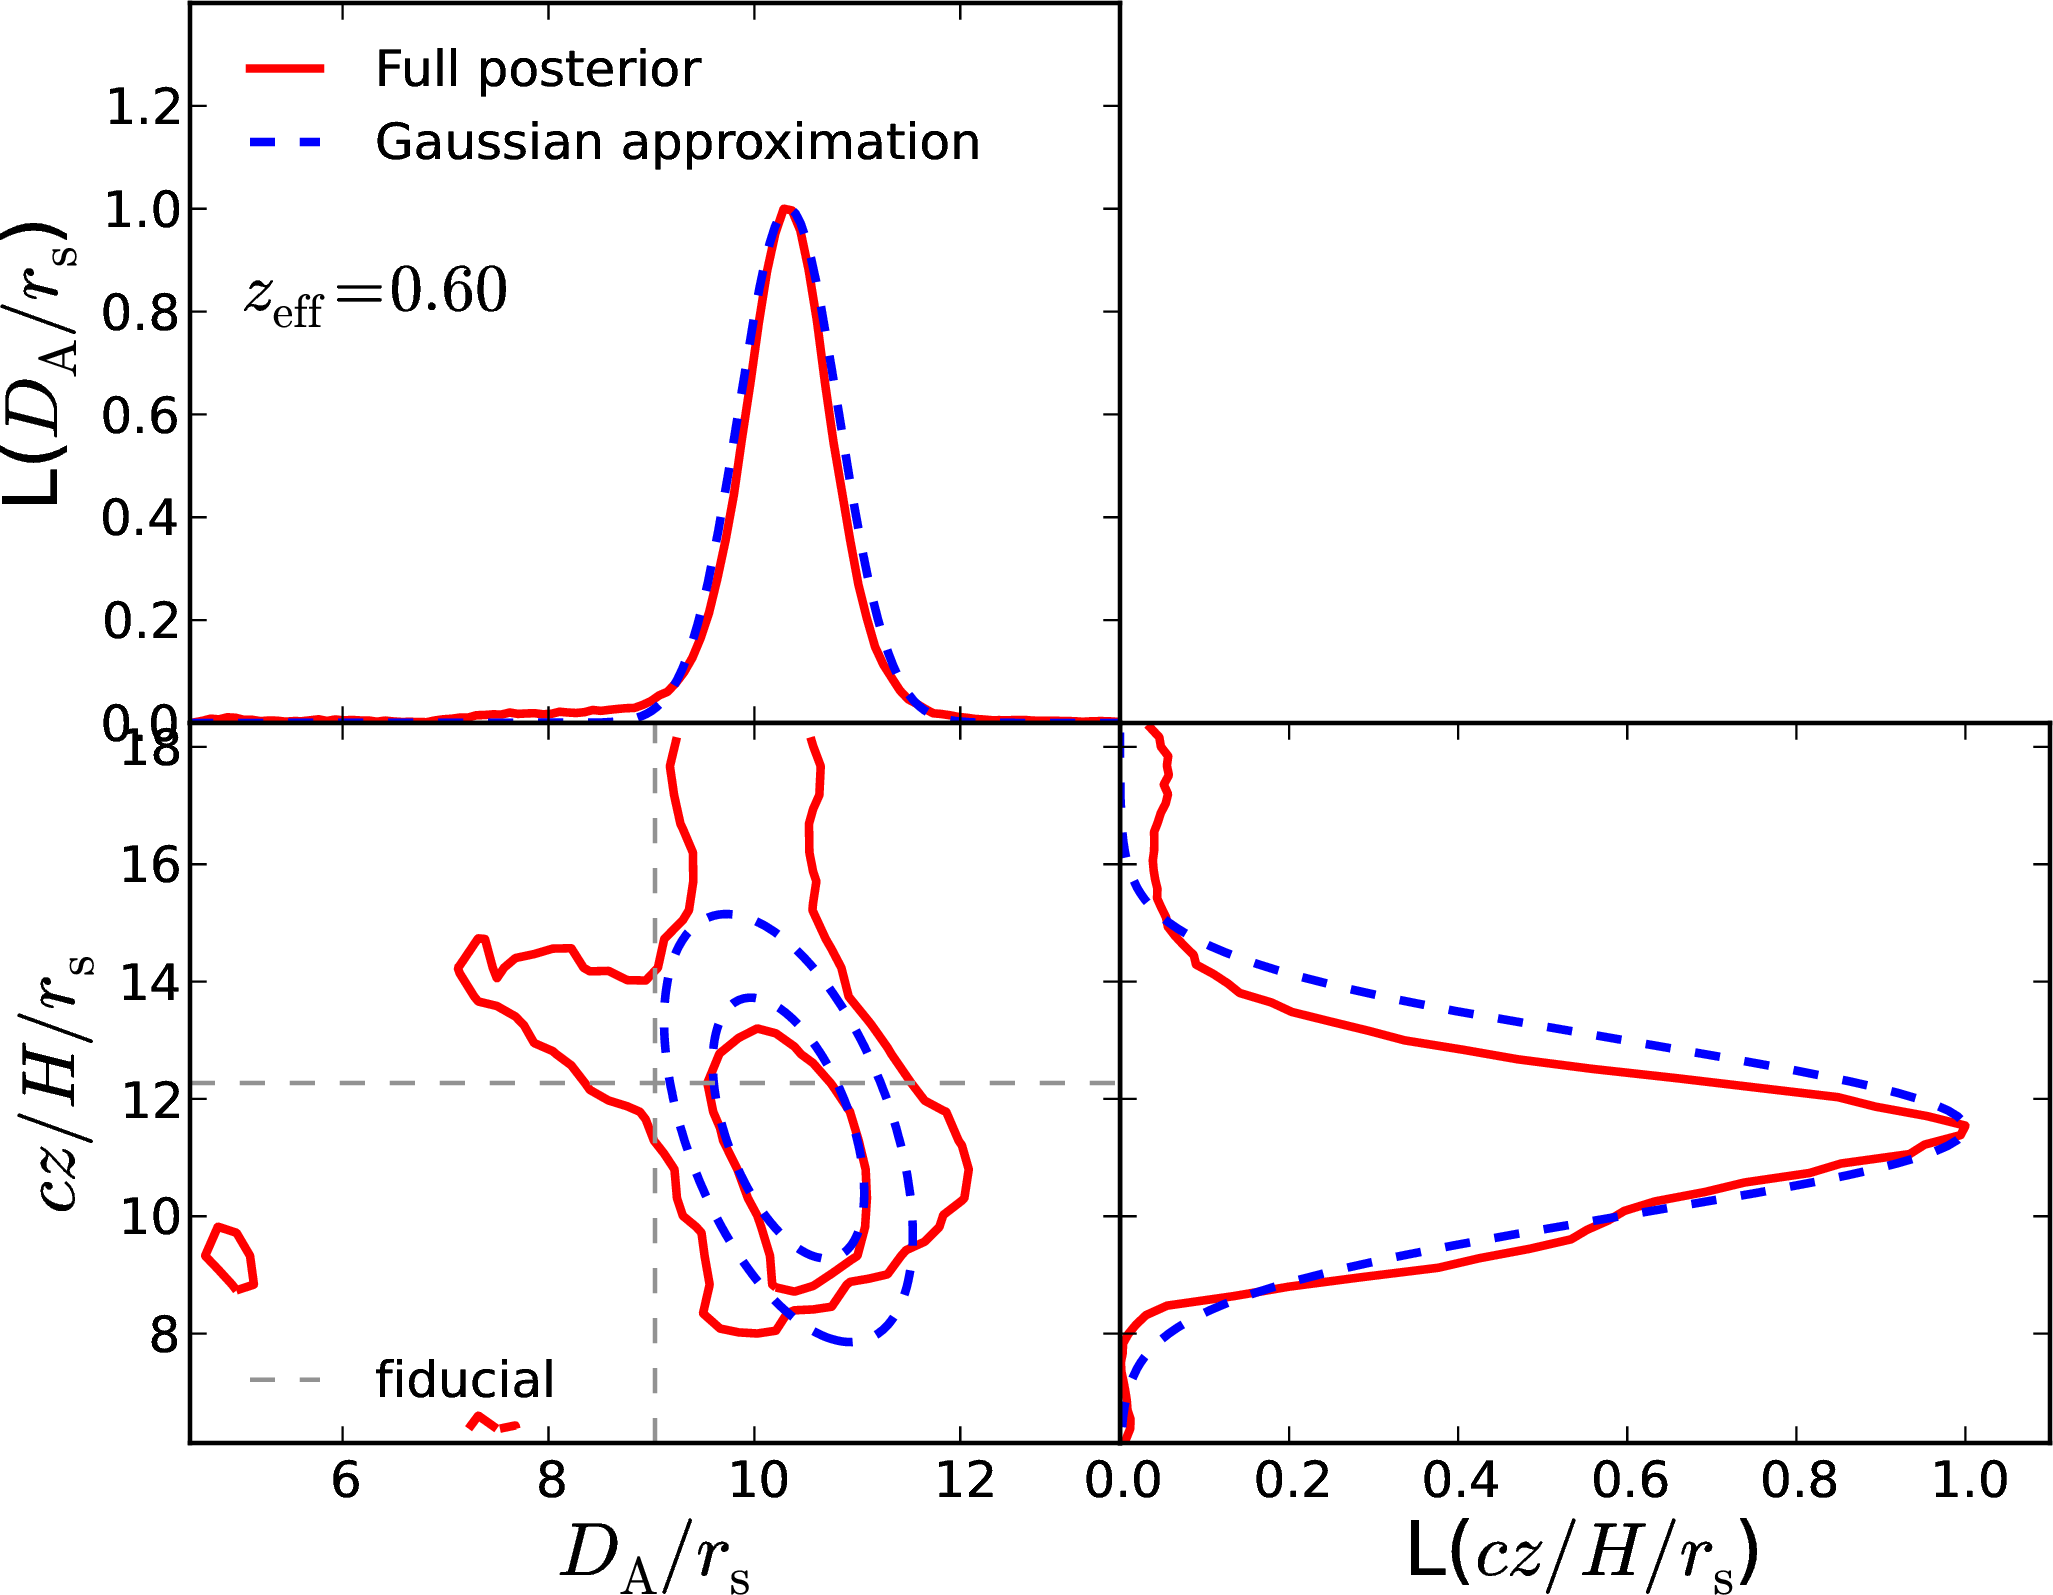
\includegraphics[width=0.9\columnwidth]{figures/stacked_L2D_rpt_wedges_postRec_T0.15_WiggleZ_z0pt4_0pt8/stacked_L2D_rpt_wedges_postRec_T015_WiggleZ_z0pt4_0pt8.png}
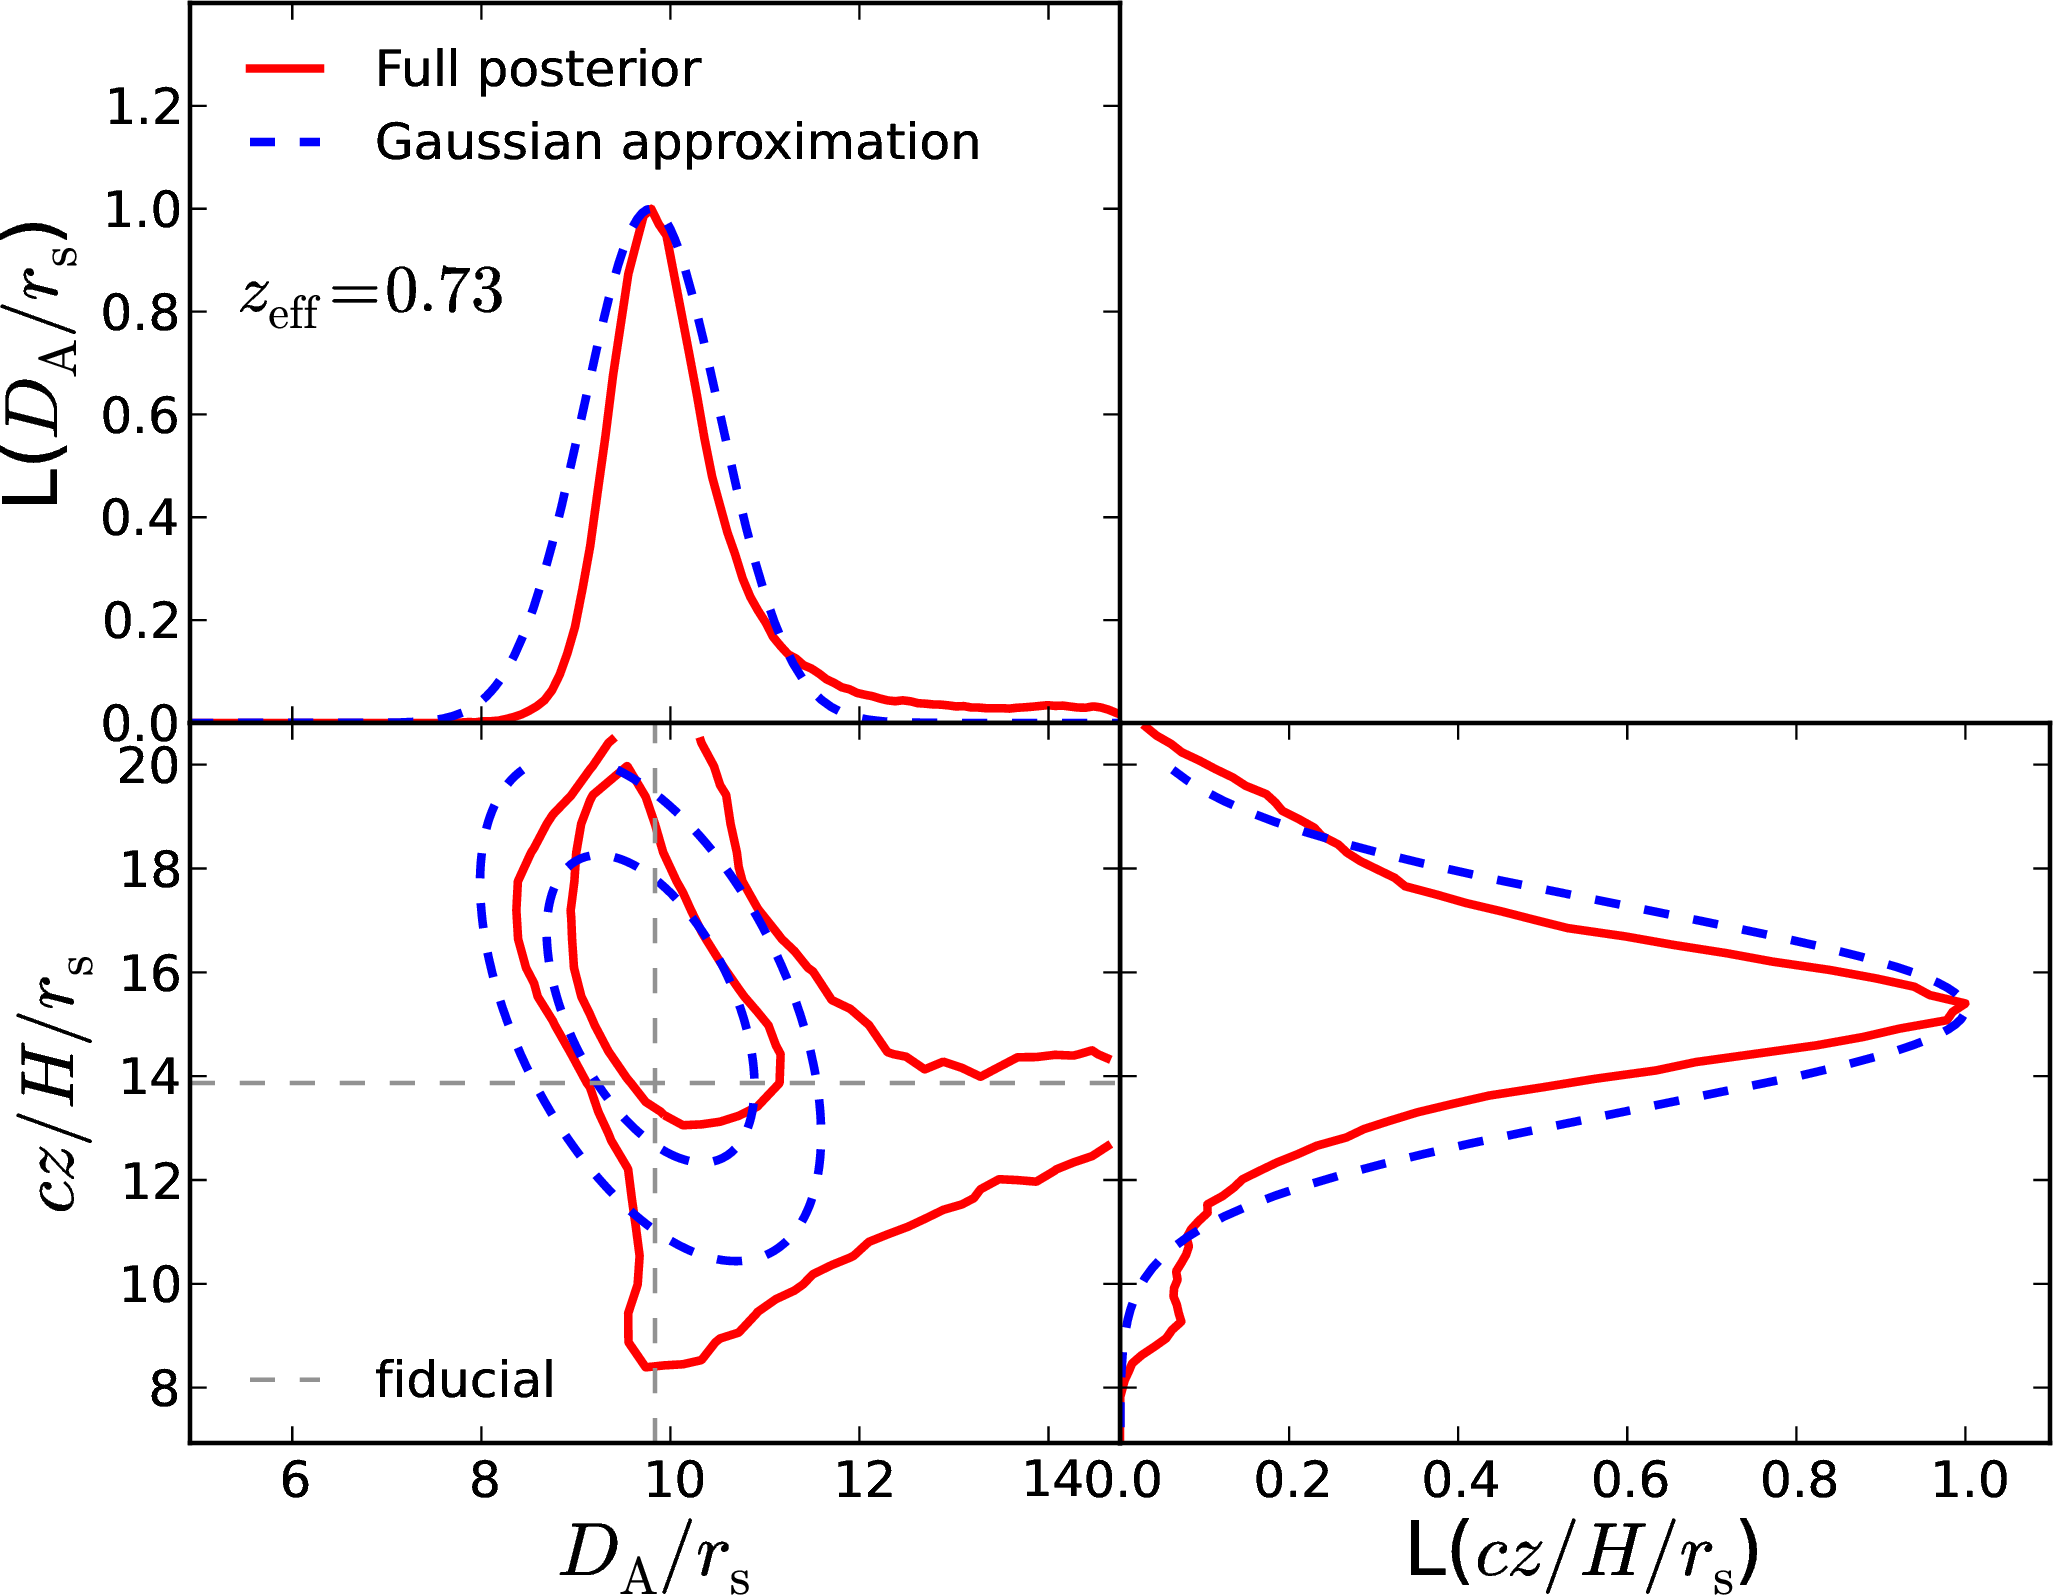
\includegraphics[width=0.9\columnwidth]{figures/z60_Model/stacked_L2D_rpt_wedges_postRec_T015_WiggleZ_z0pt6_1pt0.png}
\caption{\label{fig:HDA_z26_epsilon0.15} Marginalized posteriors of $cz/(Hr_{\rm s})$ and $D_{\rm A}/r_{\rm s}$ (red solid) obtained with WiggleZ post-reconstruction $\xi_{\perp, ||}$ in the three redshift bins $0.2<z<0.6$ (upper), $0.4<z<0.8$ (mid), $0.6<z<1.0$ (lower), using a flat prior on $\epsilon$ [-0.15,0.15].  The blue dashed lines are the Gaussian approximation when using the mode values, mean of the 68$\%$ CL regions and the cross-correlation $r$. The 2D even contours are the $68\%$ and $95\%$ CL regions and the thin gray dashed line marks the fiducial cosmology.  In the lowest redshift bin the data are not sufficient to constrain these parameters well.}
\end{center}
\end{figure}

\begin{figure}
\begin{center}
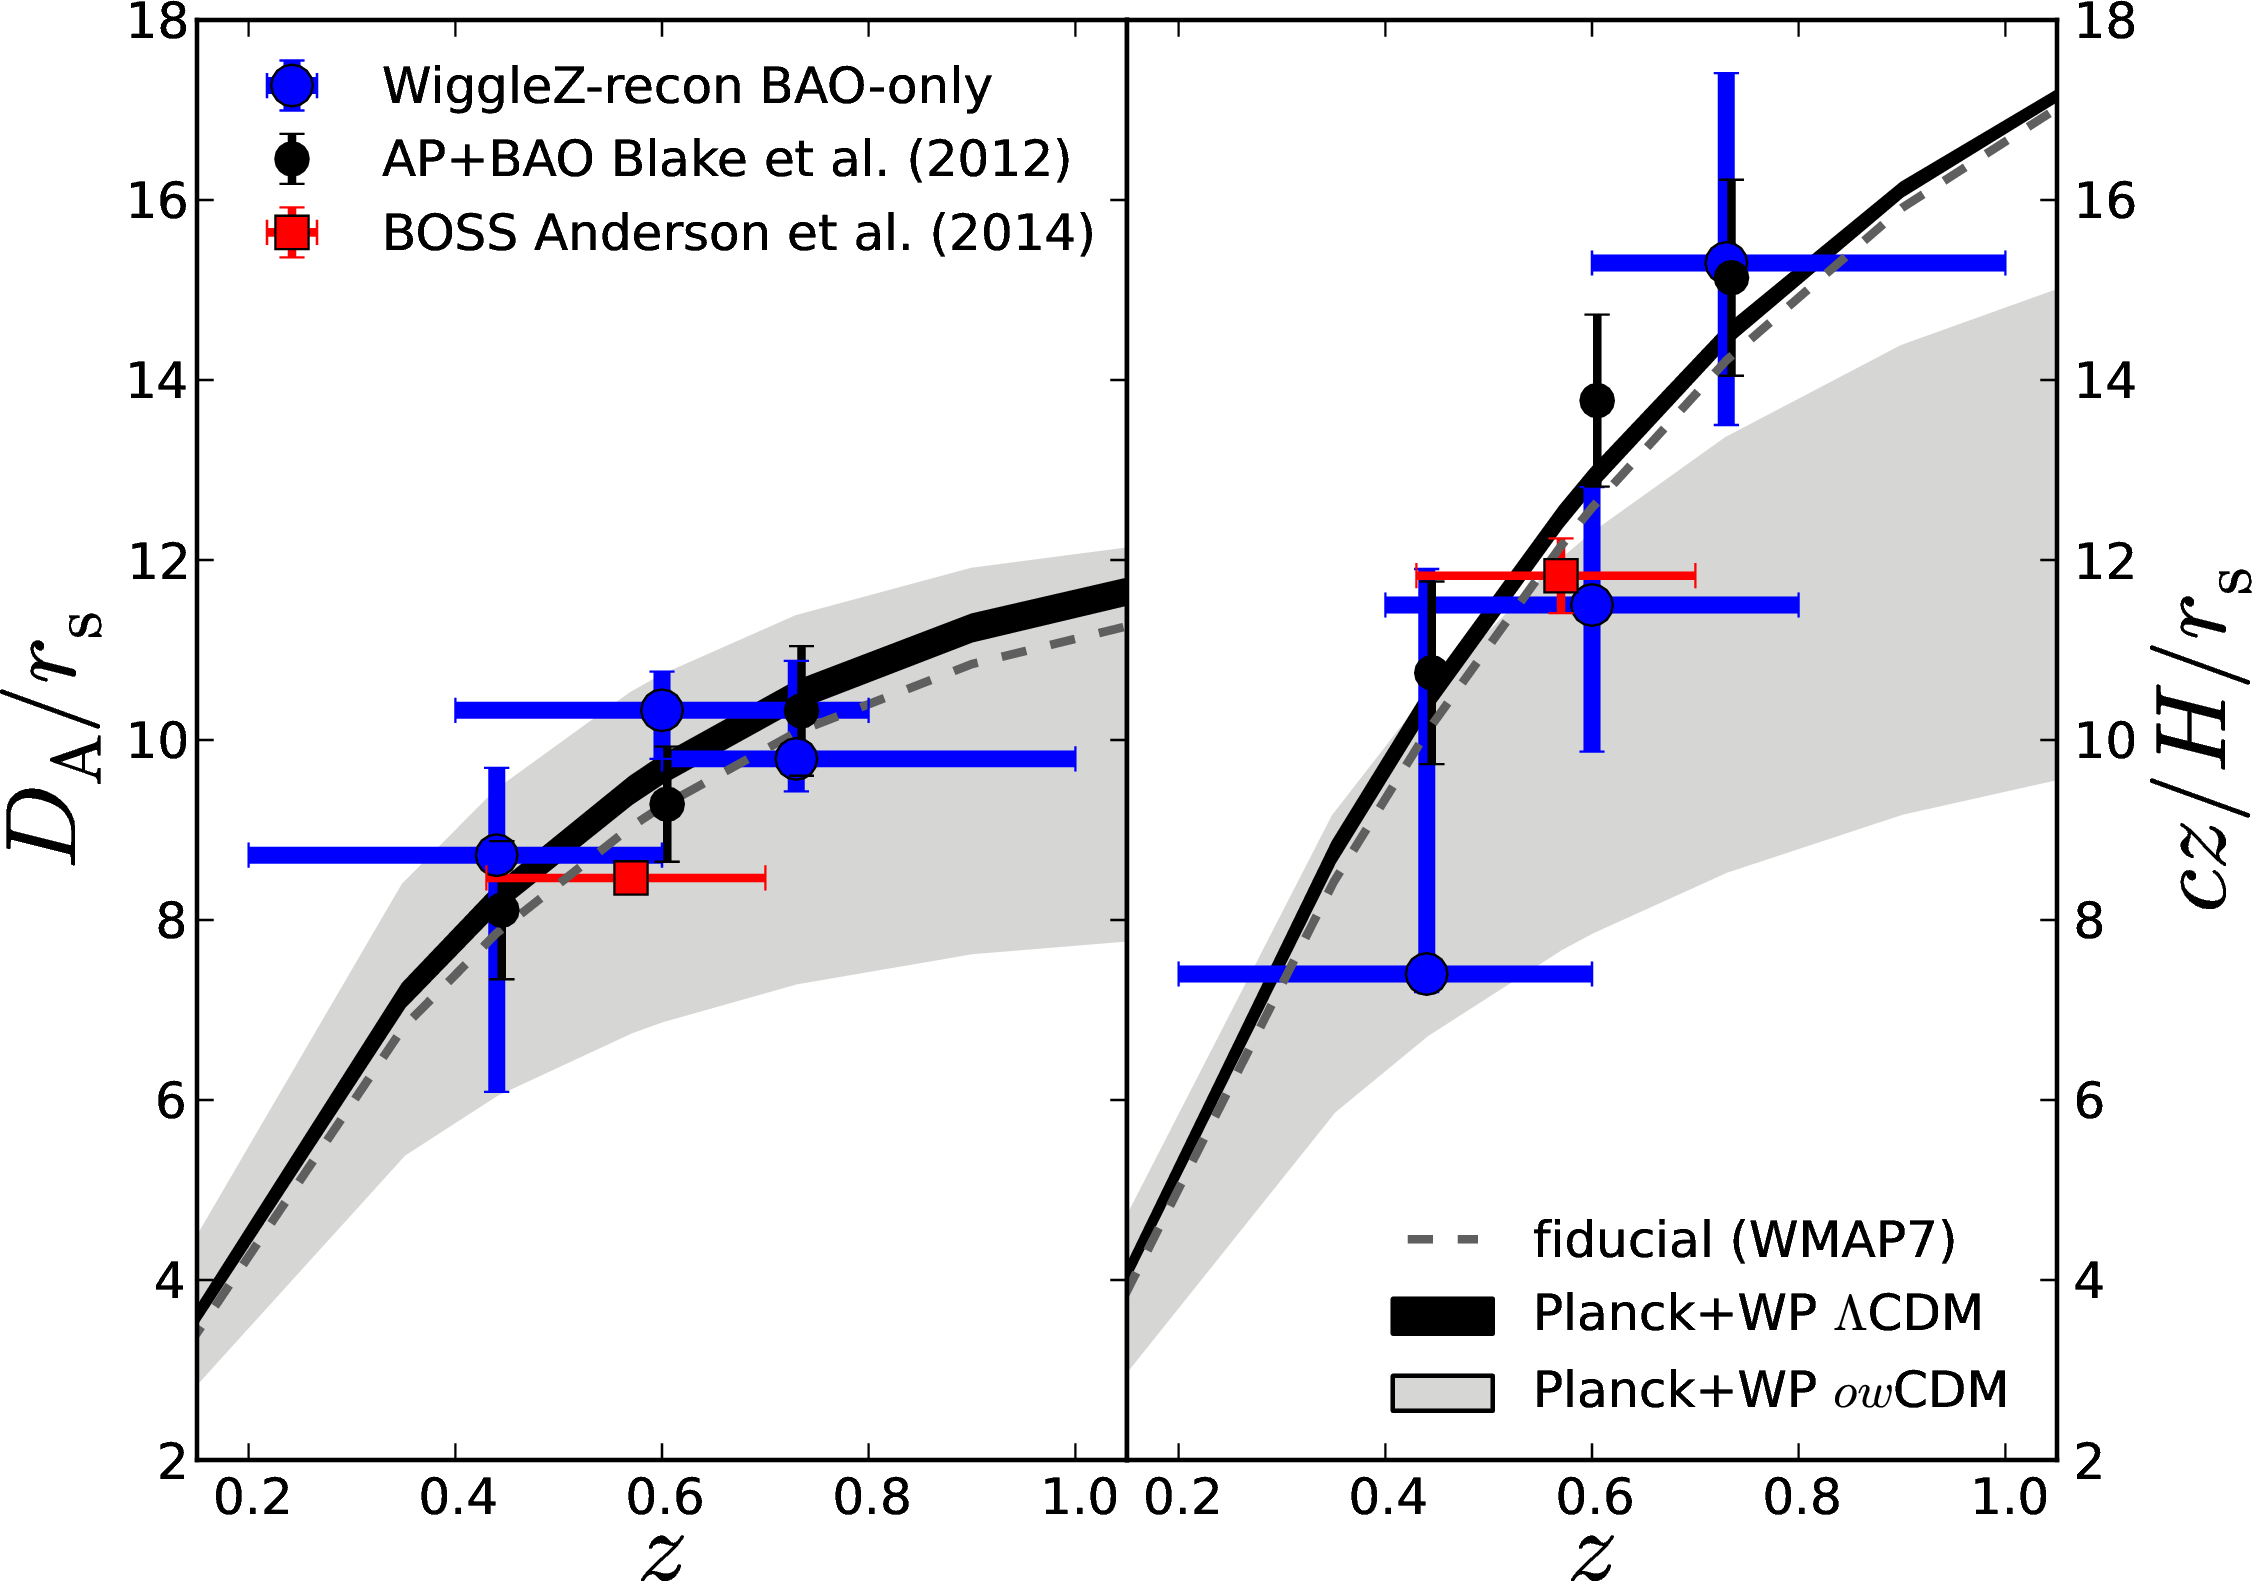
\includegraphics[width=0.7\columnwidth]{figures/hubble_HDa/hubble_HDa}
\caption{\label{fig:hubble_diagram} The WiggleZ results of $D_{\rm A}/r_{\rm s}$ (left) and $cz/(Hr_{\rm s})$ (right) in blue circles are plotted against results from AP+BAO analysis of \cite{BlakeBroughColless2012} (small black circles) and BOSS \cite{AndersonAubourg2014} (red squares), all with 68$\%$ CL regions in the $y$-axis (and redshift range on the $x$). All values are presented in Table \ref{tab:hda_wigglez_reconstructed}. The thick gray bands are $ow$CDM using Planck temperature fluctuations and WMAP9 polarization, and the thin black bands are when assuming and open $w$CDM cosmology. The dashed lines are the fiducial cosmology used in the analysis motivated by the best fit to WMAP7 data (assuming flat $\Lambda$CDM).%
{\red **PUT ON SAME DIAGRAM AS SAM'S?** }
}
\end{center}
\end{figure}










\section{Discussion and conclusion}

\label{sec:disc}
\label{sec:conclusion}

{\green **INCLUDE BOSS**}

{\red **I HAVEN'T EDITED THIS YET**  I THINK WE NEED TO ADD A SUBSECTION ON A COMPARISON BETWEEN THE TWO TECHNIQUES **}

We have presented the first measurement of the 2D BAO signal in the WiggleZ Dark Energy Survey data \citep{KazinKoda2014}, where we fit for the cosmological parameters $\Omega_c h^2$, $D_A(z)$ and $H(z)$ for the three redshift bins $z \in \left[0.44, 0.60, 0.73\right]$.  The WizCOLA simulations provided improved covariance estimates over previous analyses of the WiggleZ data which estimate covariance from lognormal realisations.

Our final constraints appear in Table~\ref{tab:wigglezBinsParams}.  These results are consistent with the Flat $\Lambda$CDM cosmology derived from best-fitting Planck cosmological values and with previous large-scale structure measurements.

In Table \ref{tab:external} and Fig.~\ref{fig:external} we show the comparison between our results and existing constraints on $D_A(z)$ and $H(z)$.  The larger uncertainty in our measurements compared to the BOSS is as-expected from the relative sizes of the data sets.  Nevertheless our results show that using a different type of galaxy tracer with much lower bias (bright blue galaxies as opposed to luminous red galaxies), we recover the same standard cosmological model. 

The main results of this analysis can be summarised as follows:
\begin{itemize}
	\item We update the unreconstructed 1D BAO measurement from \citet{BlakeKazin2011} using a more accurate covariance matrix based on WizCOLA mocks instead of lognormal realisations. The new best-fit parameters are consistent with the original measurements, with the maximum shift occurring in the highest redshift bin, whose value moved by slightly over 1$\sigma$ bringing it closer in line with the other two bins. See Table~\ref{tab:blakekazintable} for results.  Our results represent the final 1D BAO measurement using the {\em unreconstructed} WiggleZ data.  The most precise 1D BAO measurement from WiggleZ uses the {\em reconstructed} WiggleZ data as found in Kazin et al. (2014), which represents the final WiggleZ constraints from an angle-averaged BAO analysis.\footnote{{\red **CHECK WITH CHRIS: These values supersede those reported in \citet{BlakeKazin2011}, but not \citet{KazinKoda2014}}}
	\item We investigated two ways to fit the unreconstructed 2D BAO signal -- multipoles and wedges.  We found using the WizCOLA simulations that the multipoles gave a more robust result with higher statistical significance than wedges, and thus adopted multipoles for our final analysis.
	\item We validated our methodology by fitting 600 realisations of the WiggleZ survey generated by the WizCOLA simulations \citep{KodaBlake2015}. Our analysis recovered the input parameters of the simulation with no evidence for systematic bias. We also validate our methodology by testing agreement of cosmological parameters when analysing the 1D BAO signal with  \citet{BlakeKazin2011}.
	\item We thoroughly tested subtle methodological differences that could possibly have effected our analysis, such as different ways to combine the data from redshift bins, varying or fixing $\sigma_v$, or including the hexadecapole, which all gave consistent results.
	\item We performed the first cosmological analysis using the 2D BAO measurement of WiggleZ data. We detect the 2D BAO peak at a significance of slightly over 2$\sigma$ in each redshift bin. The best fit values of $\Omega_c h^2$, $H(z)$ and $D_A(z)$ are shown in Table~\ref{tab:wigglezBinsParams} and Fig.~\ref{fig:external}.  These are consistent with previous results and with the best fitting Planck cosmology and provide a consistency check on external survey results with tighter constraints from increased statistical power.
\end{itemize}






\begin{table*}
	\centering
	\caption{External constraints on $D_A(z)$ and $H(z)$. }
	%	\resizebox{\columnwidth}{!}{
	\begin{tabular}{cc|c|cc}
		\specialrule{.1em}{.05em}{.05em} 
		Paper & Source &  $z_{\rm{eff}}$ & $D_A(z)$ [Mpc] & $H(z)$ [km/s/Mpc]\\
		\specialrule{.1em}{.05em}{.05em} 
		\citet{Gaztanaga2009} {\red superseded?} & SDSS LRG DR7 & 0.24 & & $79.69\pm2.32$ \\
		& & 0.34 & &  $83.80\pm2.96$ \\
		& & 0.43 & &  $86.45\pm3.27$ \\
		
		\citet{BlakeBroughColless2012} & WiggleZ AP effect & 0.44 & $1205\pm114$ & $82.6\pm7.8$ \\
		& & 0.6 & $1380\pm95$ & $87.9\pm6.1$ \\
		& & 0.73 & $1534\pm107$ & $97.3\pm7.0$ \\
		\cite{ChuangWang2012} & SDSS LRG DR7 & 0.35 & $1048^{+60}_{-58}$ & $82.1^{+4.8}_{-4.9}$ \\
		\citet{AndersonAubourg2014DR11} & SDSS-III BOSS DR11 & 0.57 & $(1421\pm20) (r_d/r_{d,\rm{fid}})$ & $(96.8\pm3.4) (r_{d,\rm{fid}}/r_d)$ \\
		\citet{FontRiberaKirkby2014} & SDSS-III BOSS DR11 Quasars & 2.36 & $1590\pm60$ & $226\pm 8$ \\
		This paper & Wigglez 2D BAO & 0.44 & $1300\pm160$ & $87\pm16$ \\
		&   & 0.60 & $1300\pm180$ & $90\pm15$ \\
		&  & 0.73 & $1350\pm160$ & $82\pm13$ \\
		\specialrule{.1em}{.05em}{.05em} 
	\end{tabular}\label{tab:external}
	%	}
\end{table*}

\begin{figure*}[t]
	%\begin{wrapfigure}{r}{0.5\textwidth}
	\begin{center}
		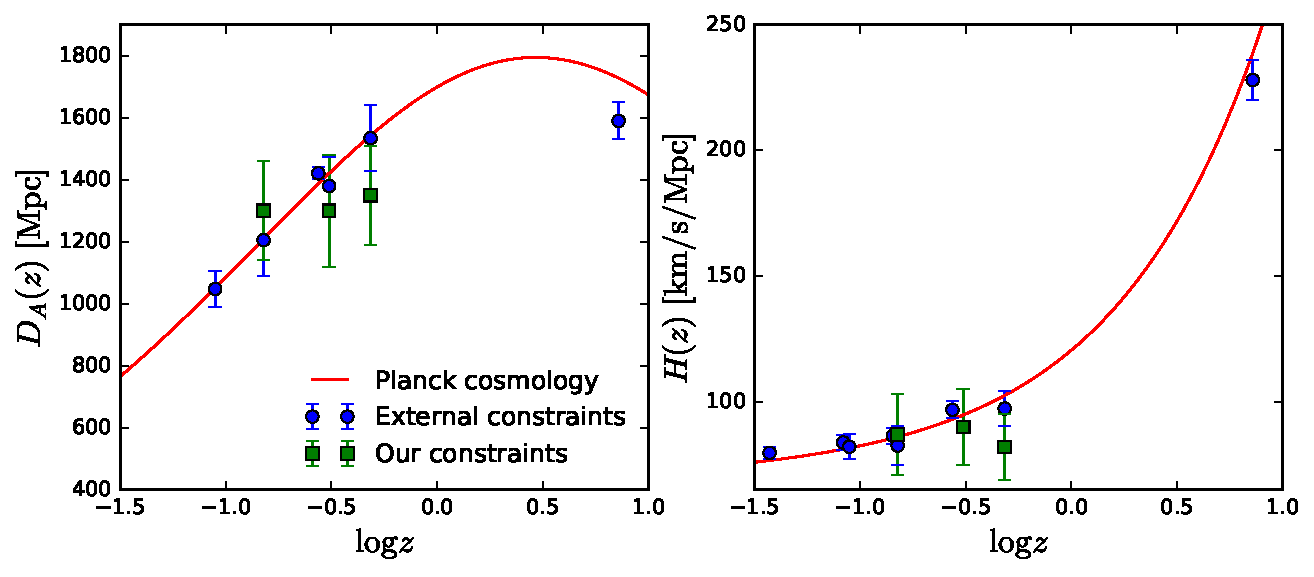
\includegraphics[width=0.9\textwidth]{images/external.pdf}
	\end{center}
	\caption{A comparison with the constraints on $D_A(z)$ and $H(z)$ found in external papers, best fitting Planck cosmology for a Flat $\Lambda$CDM universe \citep{Planck2015Parameters}, and the constraints listed in Table \ref{tab:wigglezBinsParams}.  {\red ADD EYAL'S POINTS, if they can be converted to $D_A(z)$ etc...? **} }
	\label{fig:external}
	%\end{wrapfigure}
\end{figure*}






\section*{Acknowledgments}

We gratefully acknowledge the input of the many researchers that were consulted during the creation of this paper. In particular, David Parkinson for his assistance. Sections of this work were undertaken using the NCI computer under project gi7: `Numerical simulations of stochastic galaxy formation in modified gravity theories'.   We  would also like to thank Joshua Calcino, Carolyn Wood and Sarah Thompson for their input.


\bibliography{bibliography}



\clearpage
\newpage
\phantom{df}
\pagebreak
\phantom{df}
\pagebreak
\appendix

	
	\section{Dewiggling Process} \label{app:dewiggle}
	
	In the literature the \verb;tffit; algorithm developed by \citet{EisensteinHu1998} is the most common method used to generate a power spectrum without the BAO feature. However, the use of this algorithm necessarily constrains an analysis to not only the precision of the algorithm, but also to the cosmologies considered when the algorithm was developed. Whilst most changes in cosmological models have been subtle in the past decade, a quick inspection of the changelog for CAMB\footnote{\url{http://camb.info/readme.html}} \citep{Lewis2000} shows over fifty software releases since the publication of the \verb;tffit; algorithm - representing a continual divergence between CAMB and \verb;tffit; as CAMB continues to become more accurate and consistent with modern cosmological models, whilst \verb;tffit; remains static. 
	
	Given these reasons, we decided to develop an alternate method for generating a power spectrum without the BAO feature present. Given the regular updating of the CAMB software, a replacement algorithm would be most useful if it was capable of taking a standard linear power spectrum from CAMB and returning a filtered version, such that any changes in future cosmology would be reflected in the no wiggle power spectrum simply due to its presence in the original linear power spectrum from CAMB. To this end, several different methods of filtering power spectra were investigated, implemented, and tested, and we summarise those efforts here.  For more detail see \citep{HintonThesis2015}. 
	
	\subsection{Comparison of methods}
	
	The BAO signal is present in the linear power spectrum generated by CAMB in the form of small scale oscillations after the main power peak, as illustrated in Figure~\ref{fig:ApolyDegree}. %\ref{fig:Alinear}.	
%	\begin{figure}[h]
%		\begin{center}
%			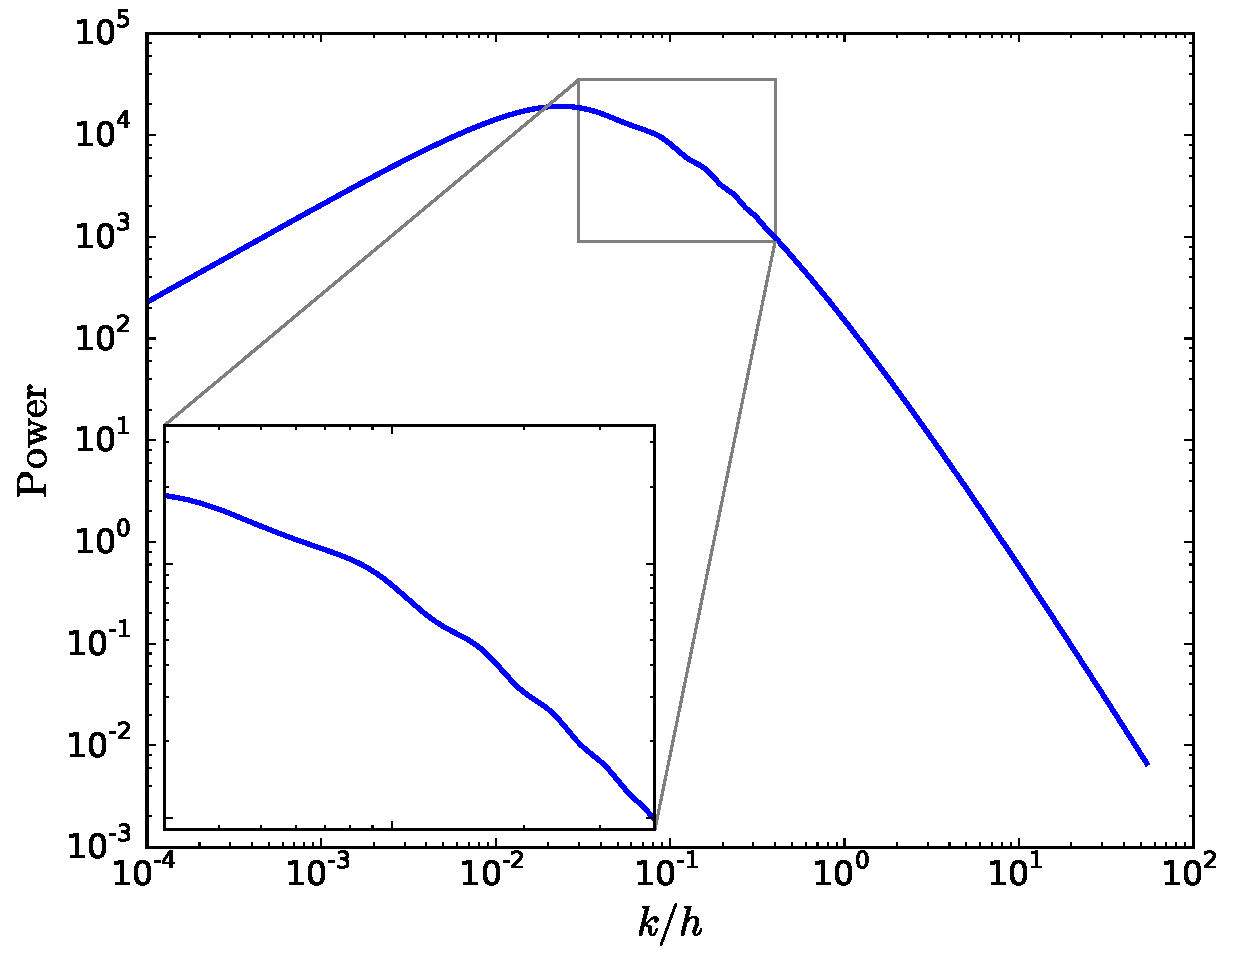
\includegraphics[width=\columnwidth]{images/Alinear.pdf}
%			\caption{A detailed look at the BAO signature present in the linear power spectrum. It presents as a set of wiggles at approximately $k/h = 0.1$.  {\red **Which cosmological model is this?  Choose one with stronger wiggles?**}}
%			\label{fig:Alinear}
%		\end{center}
%	\end{figure}	
	Given the BAO signal is of small amplitude and restricted periodicity, both polynomial data fitting, low order spline interpolation, and frequency based filtering are all viable candidates for investigation.
	We found that low-pass and band-stop filters both failed because the strong broad range signal present in the power spectrum means that signal remains present at all frequencies, and thus there were no viable filters that extracted only the BAO signal.  The two methods that were successful were polynomial regression and spline interpolation.  
	%\subsubsection{Low Pass and Band Stop Filters}	
	%It was hoped that, due to the characteristic periodicity observed in the BAO signal, it might be possible to remove it with either a low pass filter or a band stop filter. Unfortunately, the strong broad range signal present in the power spectrum (likened to a strong continuum) means that signal remains present at all frequencies, and thus there were no viable methods of extracting only the BAO signal. Figure \ref{fig:Alowpass} illustrates the difficulty of the low pass and band stop filters, namely that crushing sufficient frequencies to remove the BAO peak ends up distorting the entire shape of the power spectrum.
%	\begin{figure*}[h]
%		\begin{center}
%			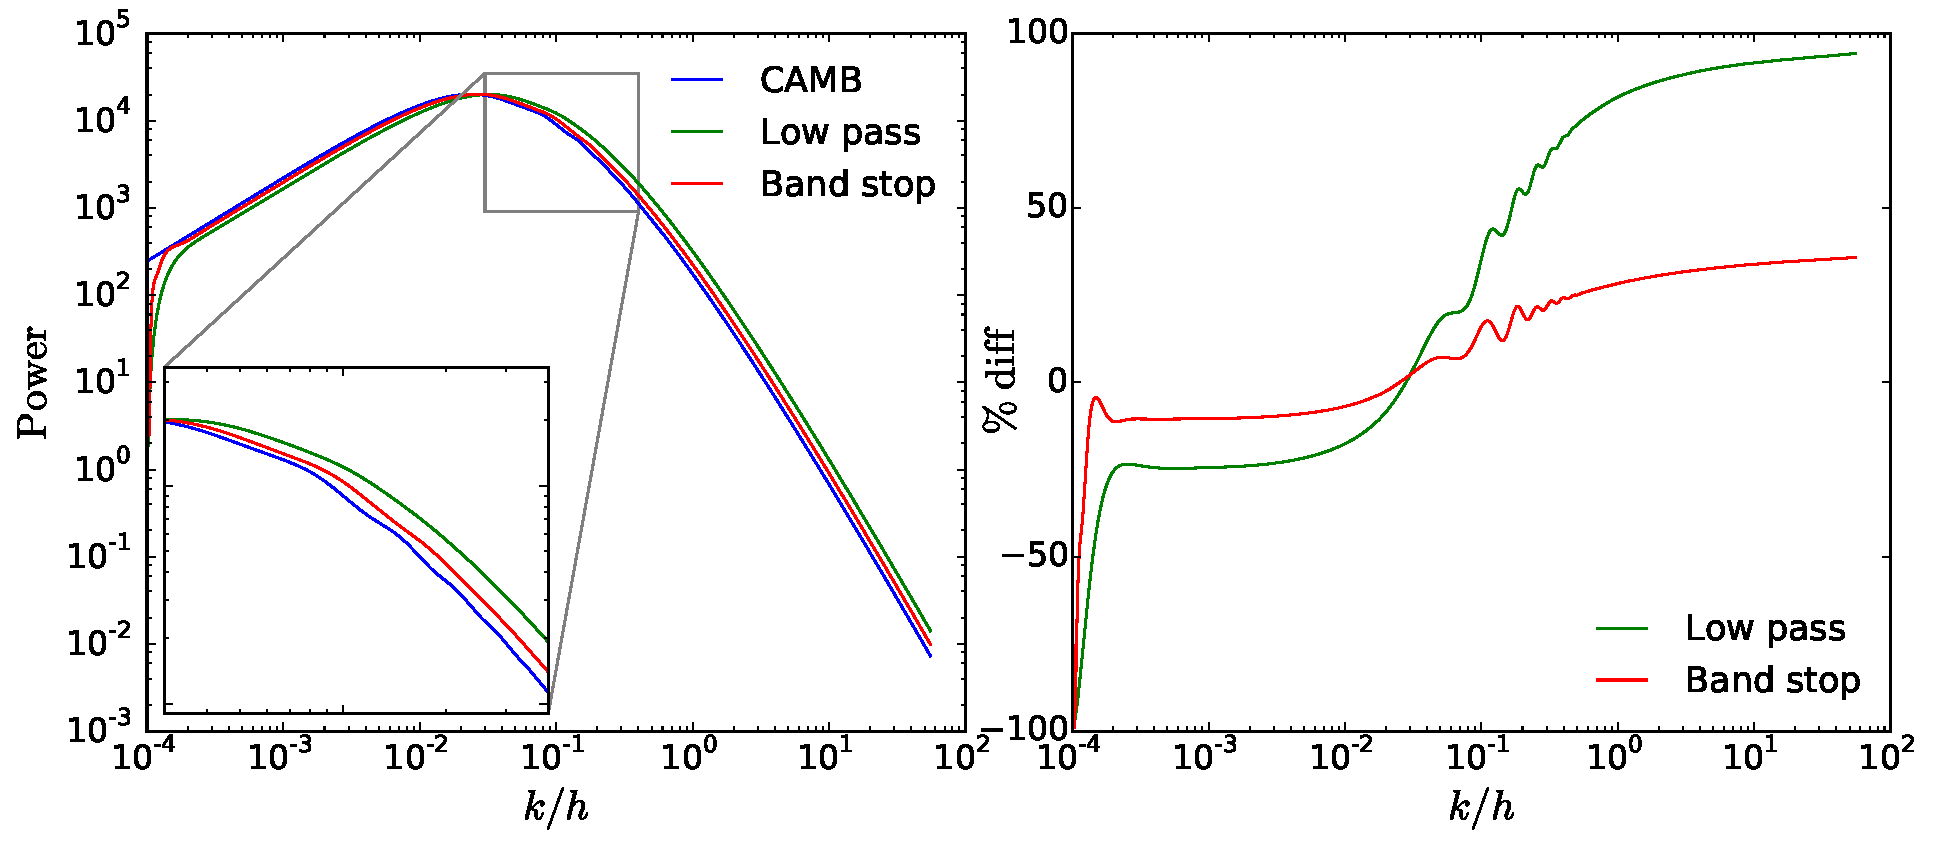
\includegraphics[width=0.8\textwidth]{images/Alowpass.pdf}
%			\caption{Herein lies the failed attempts at using an easily available digital signal processing library to remove the BAO signal without changing the broad power spectrum.}
%			\label{fig:Alowpass}
%		\end{center}
%	\end{figure*}
	
	\subsubsection{Polynomial regression}
	
	Polynomial regression are a tried and tested method for determining broad shape in a given spectrum \citep{baldry2014galaxy}. The higher order the polynomial fit becomes, the better the broad band shape extraction becomes, at the cost of eventually, as one keeps increasing the order, the polynomial model becomes detailed enough it begins to recover BAO signal. To counter this, one can introduce weights on the points, where the data points in the range of the BAO wiggle are down weighted. To make this method more viable, a specific $k/h$ is not chosen as the centre point (as this strongly removes our model independence), instead we can note that the wiggle will appear approximately at the data peak, and down weight this area using a Gaussian weighting function, such that the weights supplied to the polynomial regression take the form $w = 1 - \alpha \exp\left(-k^2/2 \sigma^2\right)$. Using this, we can construct an array of polynomial fits where the polynomial degree, Gaussian width and amount of down weighting are varied to determine the most effective construction to remove the BAO signal. In order to take advantage of the smooth shape of the power spectrum in the log domain, the polynomial regression is applied to the logarithm of the power spectrum.
	
	
	\begin{figure*}
		\begin{center}
			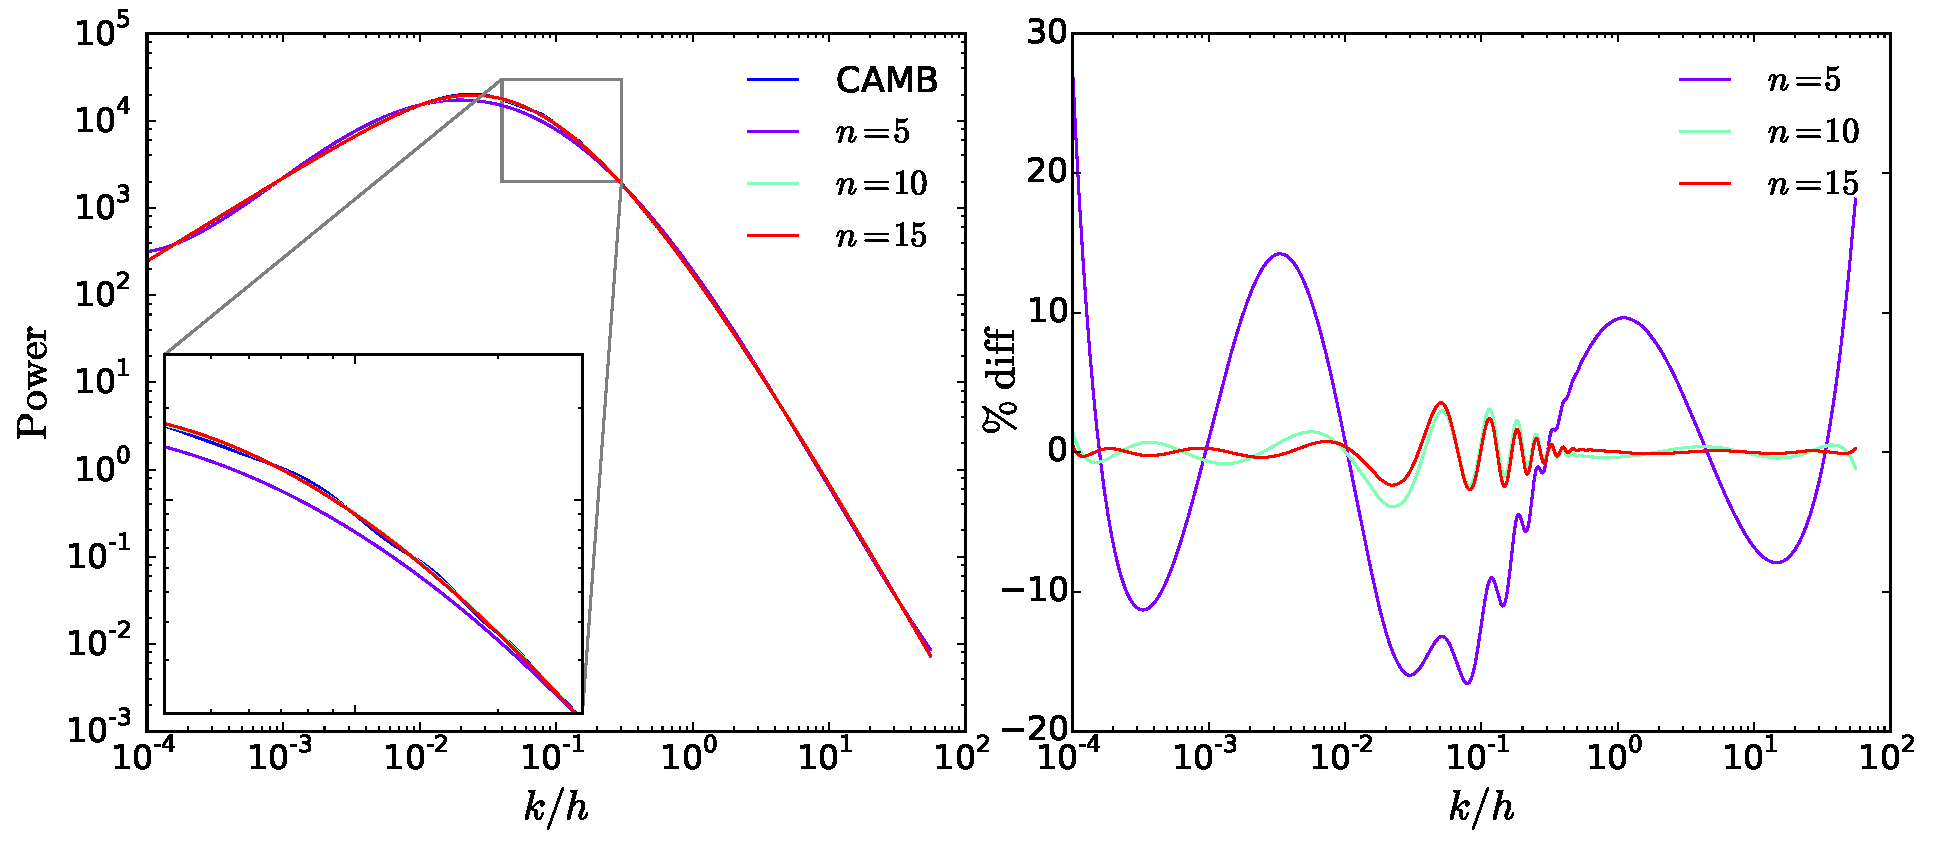
\includegraphics[width=0.7\textwidth]{images/ApolyDegree.pdf}
			\caption{A comparison of the effects of increasing polynomial weight. Due to the high number of data points in the linear CAMB model ($>600$), even a high degree polynomial such as the 15 degree polynomial displayed in red, does not attempt to recover the BAO signal. Given the range of $k_*$ values typically used in model fitting, the right hand side of the graph where $k/h > 0.1$ is most relevant. It is desired that the polynomial fit converge to the CAMB power spectrum at high $k/h$, as occurs with higher order polynomial fits.}
			\label{fig:ApolyDegree}
		\end{center}
	\end{figure*}
	\begin{figure*}
		\begin{center}
			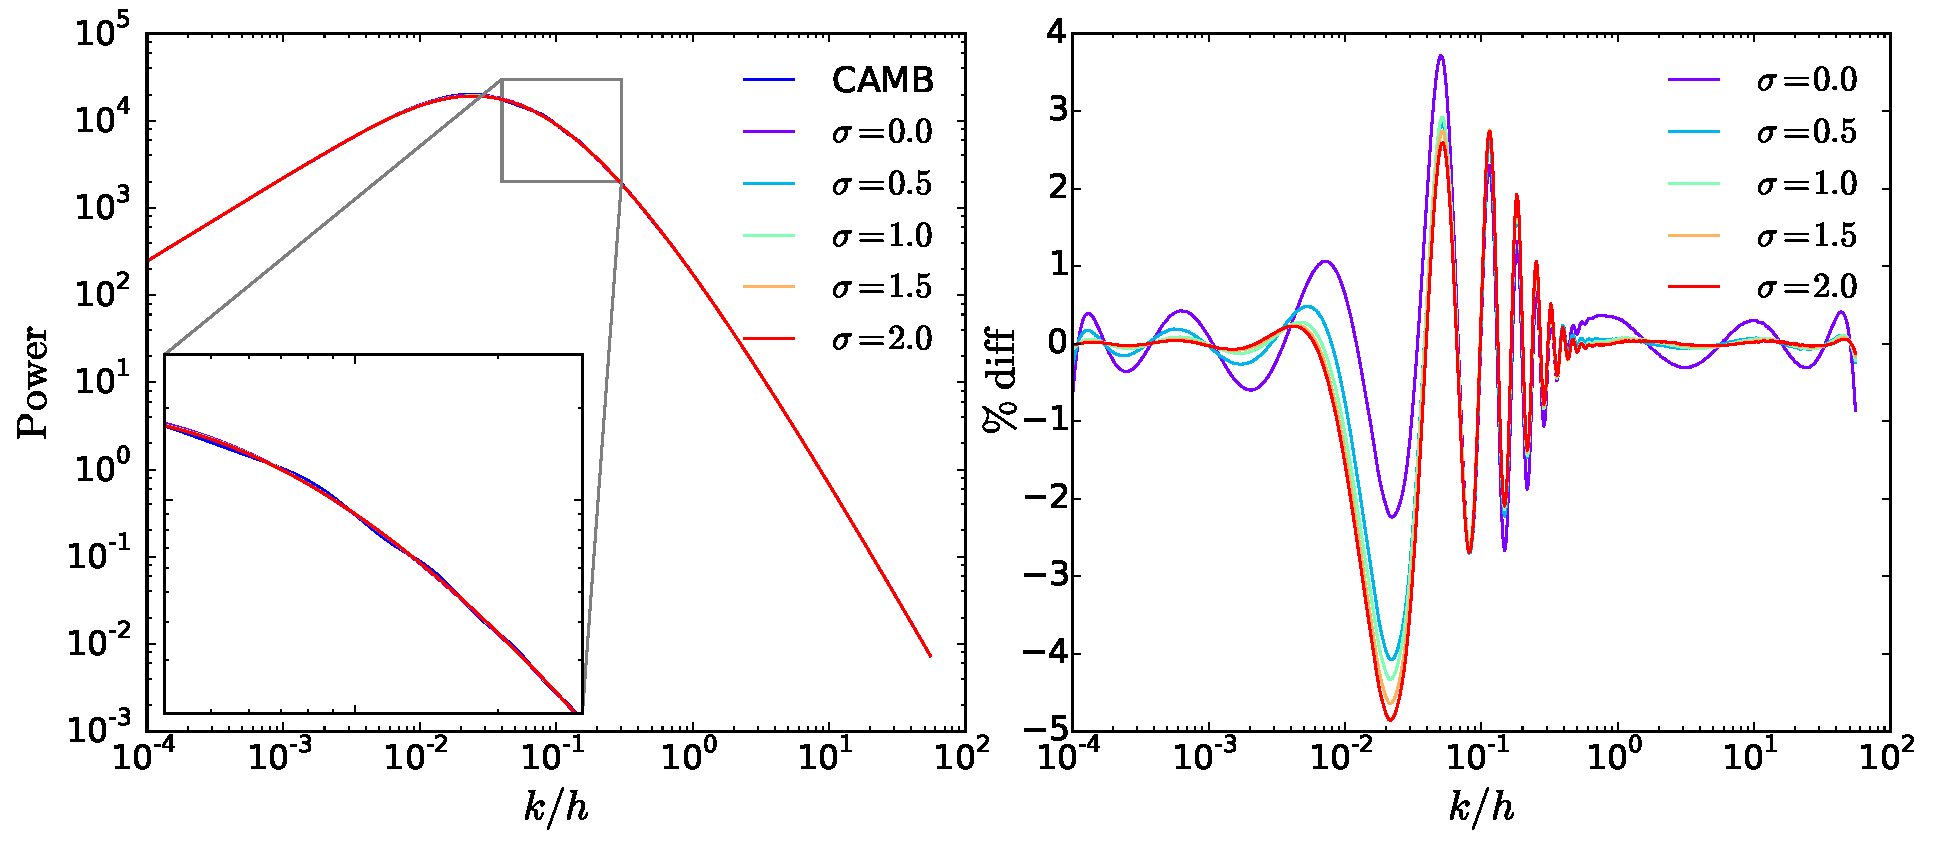
\includegraphics[width=0.7\textwidth]{images/ApolySigma.pdf}
			\caption{With polynomial degree fixed to $n = 13$, the width of the Gaussian used to down weight the peak of the spectrum is compared in this plot. It can be seen that no Gaussian ($\sigma= 0.0$) results in oscillations at high $k/h$, whilst the increasing $\sigma$ initially leads to better convergence at high $k/h$, with continually increasing $\sigma$ reducing the completeness of the BAO signal subtraction.}
			\label{fig:ApolySigma}
		\end{center}
	\end{figure*}
	\begin{figure*}
		\begin{center}
			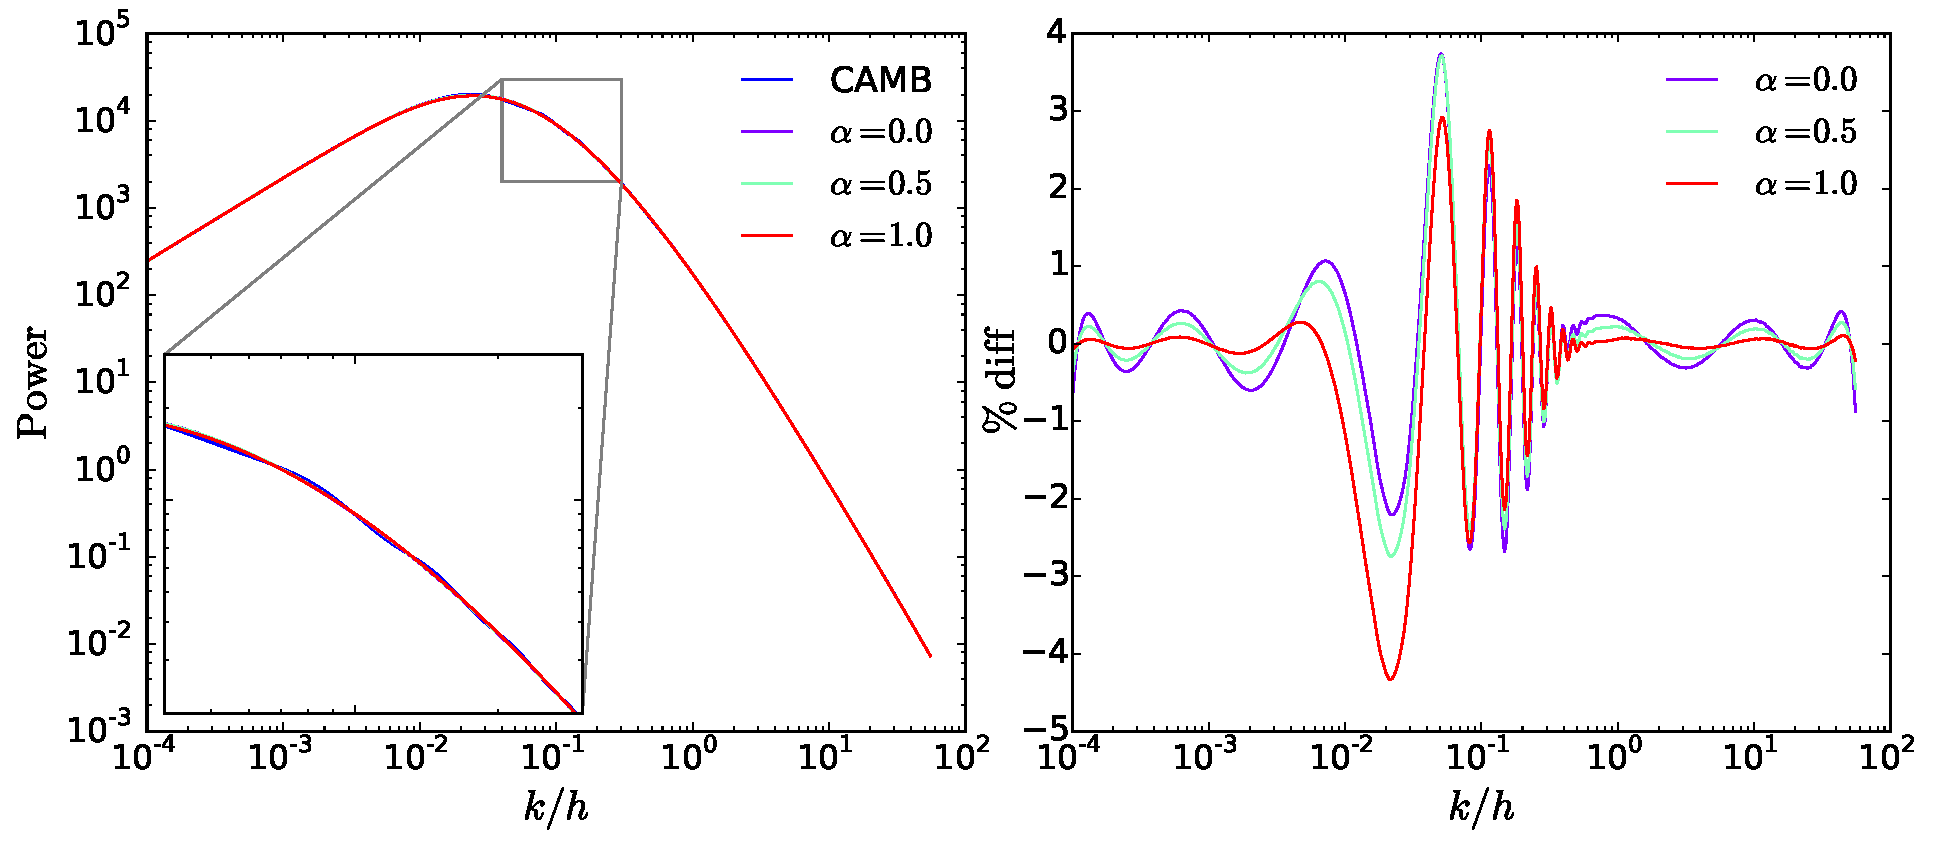
\includegraphics[width=0.7\textwidth]{images/ApolyWeight.pdf}
			\caption{Setting $\sigma = 1$, we can examine the effect of the weight $\alpha$ of the Gaussian down weighting. As expected, setting the weight to zero gives the oscillations at high $k/h$ found in Figure \ref{fig:ApolySigma}. Setting the subtraction to full strength with $\alpha = 1.0$, we see that there is a downward shift in the polynomial fit (as the peak which lifts the fit has effectively been removed). Thus a compromising value in between must be chosen.}
			\label{fig:ApolyWeight}
		\end{center}
	\end{figure*}
	
	
	By comparing a wide array of parametrisations of polynomial degree $n$, Gaussian width $\sigma$ and Gaussian weight $\alpha$, a final combination of $n=13, \sigma=1, \alpha=0.5$ we chosen to act as the best choice for both strong BAO signal subtraction and non distortion of the original linear power spectrum.

	
	\subsubsection{Spline Interpolation}
	
	
	The final method of removing the BAO signal from the linear power spectrum investigated was using spline interpolation. Similarly to the polynomial fits, it has the option of being supplied relevant weights for each data point, and thus a similar investigation as to weights was carried out for spline interpolation as was carried out for polynomial fitting. The spline fitting was found to be completely insensitive to modified weights, but highly sensitive to the positive smoothing factor $s$. A value of $s = 0.18$ compromises between BAO subtraction and low levels of distortion at high $k/h$, as determined by minimising the difference between the resultant spline model and the output of \verb;tffit;. Spline interpolation was similarly investigated in \citet{ReidPercival2010}, who found that use of a cubic b-spline with eight nodes fitted to $P_{\rm{lin}}(k) k^{1.5}$ produced likelihood surfaces in high agreement with formula from \citet{EisensteinHu1998}. In testing this methodology for potential use, no benefit was found to come from rotating the power spectrum via the $k^{1.5}$. This was found for both tests using a univariate spline and a b-spline, however the similarity between the results of the different splines was such that only the univariate spline is documented.
	
	
%	\begin{figure*}[h!]
%		\begin{center}
%			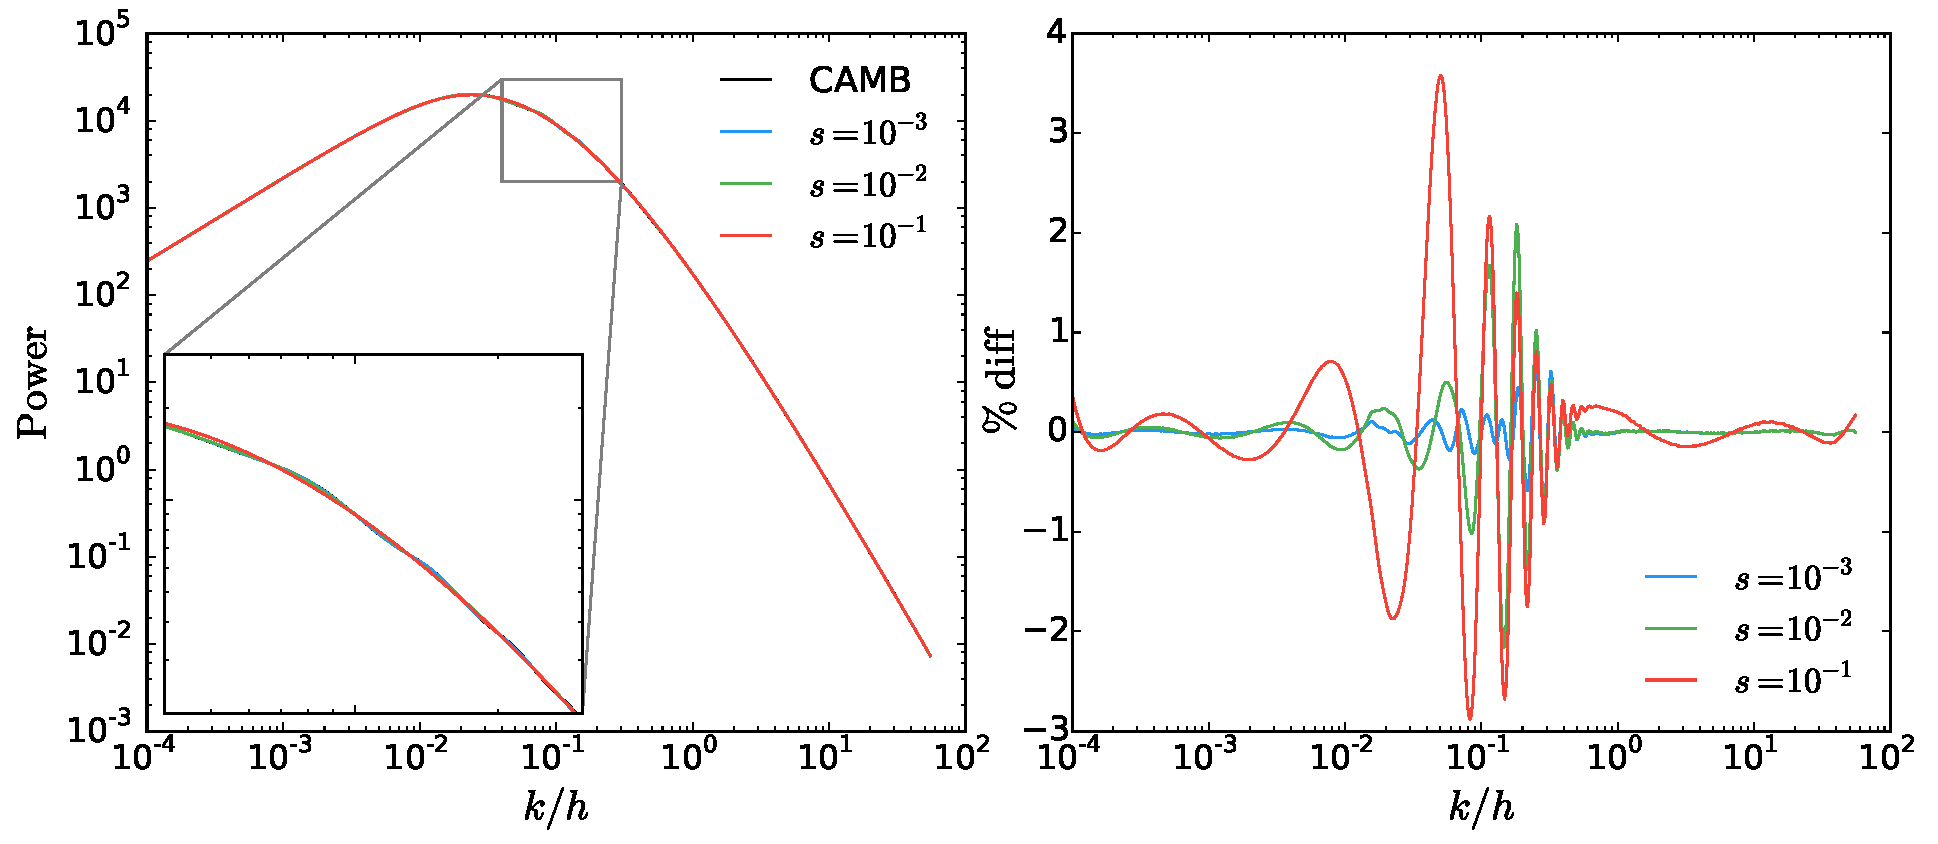
\includegraphics[width=0.8\textwidth]{images/AsplineSmooth.pdf}
%			\caption{Modifying the positive smoothing factor $s$ when computing a 5-point univariate spline has dramatic effects on the extraction of BAO signal. Setting $s < 0.01$ stops the spline from effectively removing the BAO signal, whilst setting it higher such that $s > 0.3$, the deviation from the linear power spectrum starts becoming significant at higher $k/h$ values.}
%			\label{fig:AsplineSmooth}
%		\end{center}
%	\end{figure*}
	
	\subsection{Selection of final model}
	
	Selecting the final method of dewiggling input spectra was done via looking explicitly at how the spectra are used in cosmological fitting: they are transformed into correlation functions and compared to observed data points. As such, the chosen optimal configurations for the polynomial and spline method were compared to \verb;tffit; by performing a cosmological sensitivity test wherein fits to WizCOLA data using the polynomial method, spline method and the algorithm given by \citet{EisensteinHu1998} are directly compared. To ensure this is robust, the value $k_*$ is fixed to 0.1, representing a fit with a very high level of dewiggling (hard thresholds are often limited to around this value, ie \citet{ChuangWang2012} have minimum $k_* = 0.09$), whilst still preserving some of the BAO peak with which to match. This analysis is given in Figure \ref{fig:AcosmologyTest}, and shows that for both spline and polynomial methods outlined above, statistical uncertainty in fits far exceeds any difference in matching results due to the change in dewiggling process. The polynomial method was selected to be the final method, due to the observed roughness in spline fitting which is the result of the changing dependence on the positive smoothing factor.
	
	
	\begin{figure}[t]
		%\begin{wrapfigure}{r}{0.5\textwidth}
		\begin{center}
			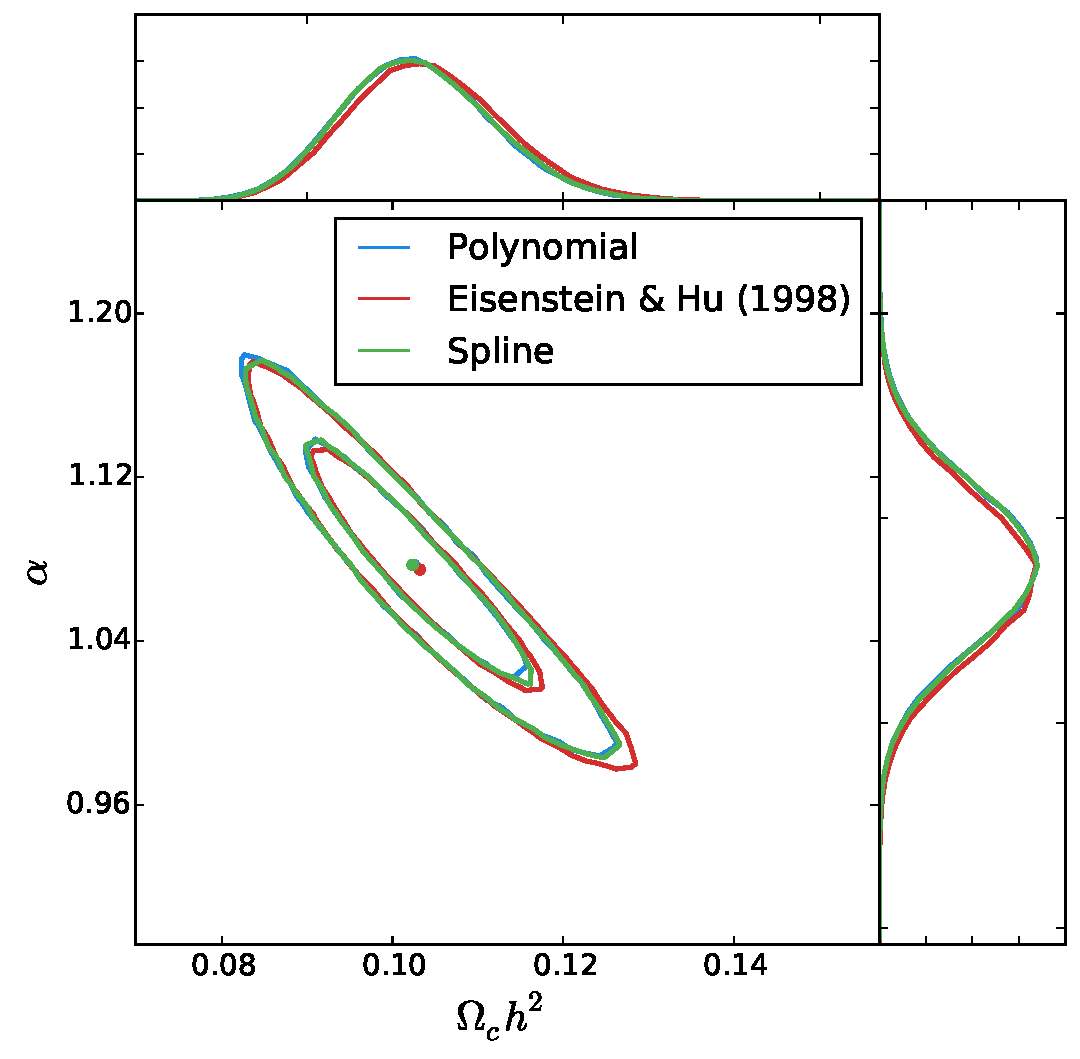
\includegraphics[width=\columnwidth]{images/AcosmologyTest.pdf}
		\end{center}
		\caption{A cosmological sensitivity test between the algorithm from \citet{EisensteinHu1998}, polynomial fitting and spline fitting. Likelihood surfaces and marginalised distributions were calculated using the WizCOLA simulation data at the $z=0.6$ redshift bin, where all 600 realisations have been used as input data, and $k_*$ fixed to $0.1$. With the low value of $k_*$ to increase the significance of the dewiggling algorithm and high data quality to reduce statistical uncertainty beyond the scope of the WiggleZ dataset, any deviation between the different methodologies should represented in the likelihood surfaces represents extremal values of diverge. However, as all likelihood surfaces agree to a high degree, we can conclude any difference in methodology is negligible in comparison to statistical uncertainty.}
		\label{fig:AcosmologyTest}
		%\end{wrapfigure}
	\end{figure}
	
	
	









\begin{comment}
\section{Improving computation speed from Power Spectrum to Correlation Function} \label{app:pk2xi}

The monopole moment of the power spectrum obtained in model creation is analytically transformed to a correlation function via the first order three dimensional Fourier transformation 
\begin{align} \label{eq:she}
\xi(s) = \frac{1}{(2 \pi)^3} \int 4 \pi k^2 \, P(k)\,  \frac{\sin(ks)}{ks}.
\end{align}
Unfortunately, non-linear growth of the power spectrum at high $k$ hinders convergence of numerical computation of the correlation function. In this section, we test two methodologies to increase convergence, respectively from \citet{BlakeDavis2011} and \citet{AndersonAubourg2012}, against a high quality (and thus exceedingly slow) numerical method to determine the effect the modified algorithms have on the final model.

\begin{figure}[t]
	%\begin{wrapfigure}{r}{0.5\textwidth}
	\begin{center}
		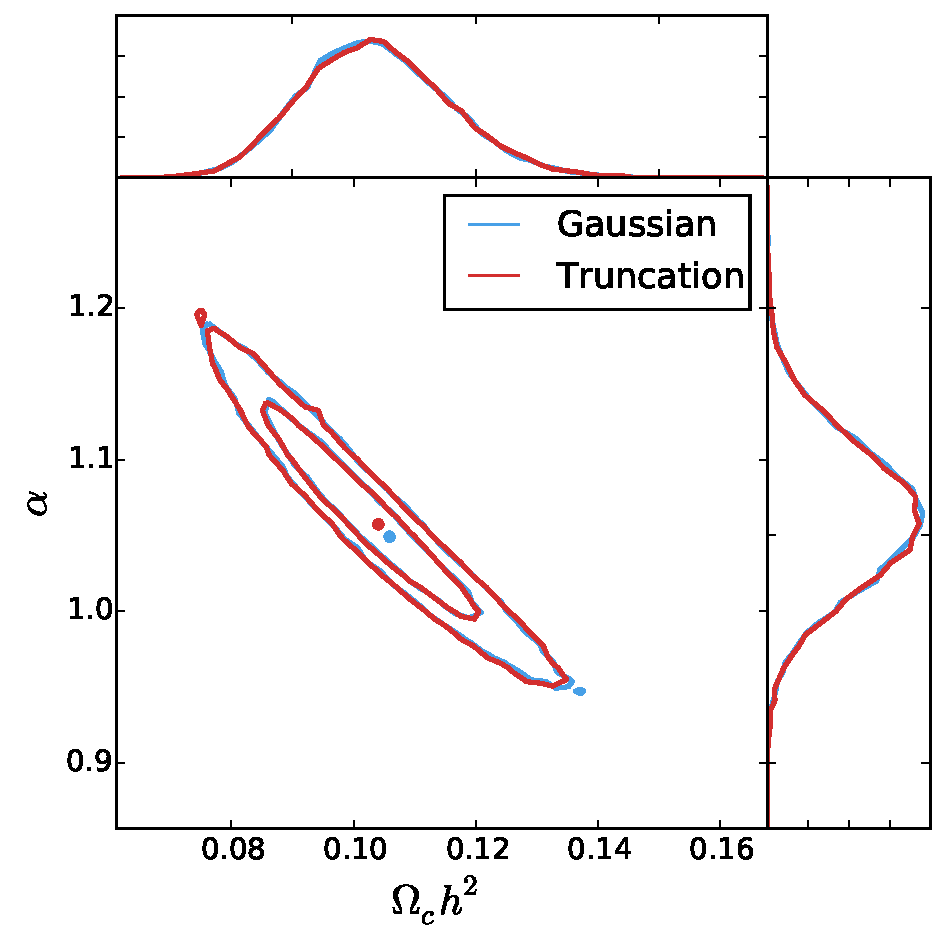
\includegraphics[width=\columnwidth]{images/BcosmoComp.pdf}
	\end{center}
	\caption{Likelihood surfaces for $1\sigma$ and $2\sigma$ confidence levels and marginalised distributions were created using both the Gaussian $a=0.5$ and truncated method of moving from a power spectrum to a correlation function. Models were compared to the combined monopole moment of the 600 WizCOLA simulations in the $z=0.4$ redshift bin. Parameters $\beta, b^2, k_*, \sigma_V H(z)$ are marginalised over in these MCMC fits. Data noisiness exists from halting the MCMC algorithm early (2 million steps combined) after it became clear the two methods gave negligible differences.}
	\label{fig:BcosmoTest}
	%\end{wrapfigure}
\end{figure}


\begin{figure*}
	%\begin{wrapfigure}{r}{0.5\textwidth}
	\begin{center}
		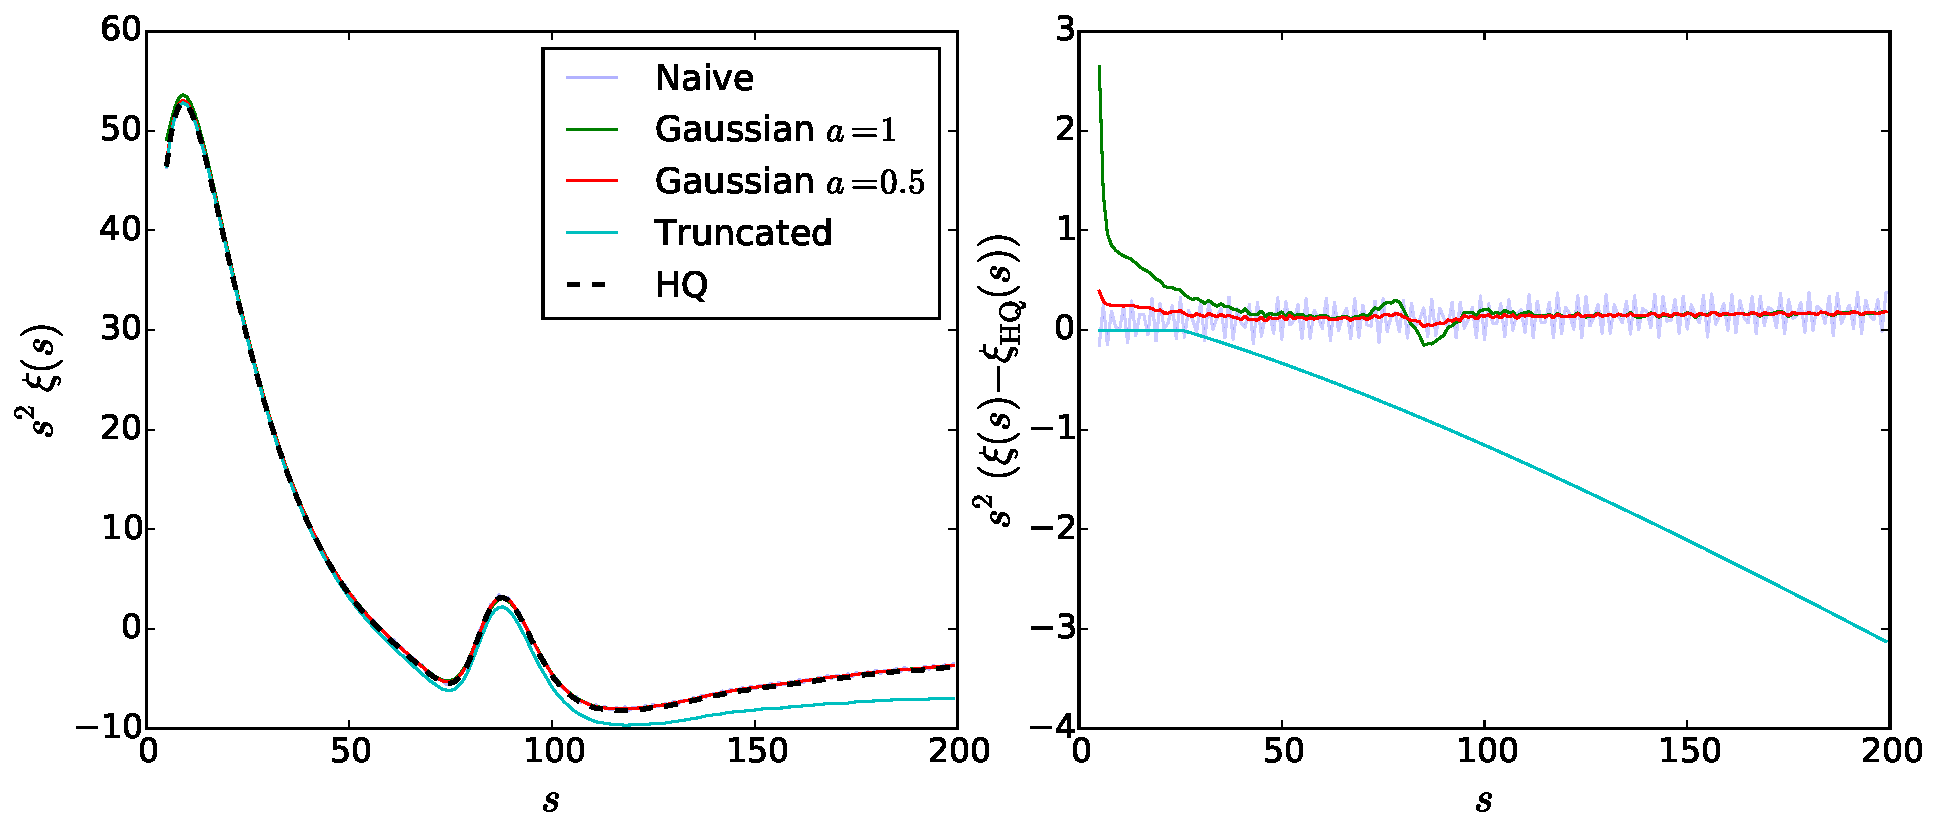
\includegraphics[width=0.8\textwidth]{images/Bxi.pdf}
	\end{center}
	\caption{A comparison of the different algorithms used to perform the numerical Fourier transformation. The power spectrum supplied to the algorithms consisted of 732 data points ranging up to $k = 223.56 \ h/$Mpc. The oscillations present in the naive spectrum are due to the fact the integration bounds are not infinite, and form due to the cumulative effect of the $\sin(ks)$ term when the integration bounds truncate the calculation when $\sin(ks) \neq 0$. The Gaussian method used by \citet{AndersonAubourg2012} with $a=1$ provided good convergence to the high quality algorithm at $s > 20 h^{-1}$ Mpc, with a slight deviation around the BAO peak itself and a general positive offset of approximately of $\Delta = 0.1 s^2 \xi(s)$ (which has negligible impact on cosmological fitting due to the marginalisation over power amplitude from $b^2$). Both the initial deviation and the peak deviation were greatly reduced in magnitude when $a$ was set to $0.5$ instead of $1$. The greatest deviation from the high quality algorithm was found by the truncated algorithm used in \citet{BlakeDavis2011}, where the truncation increased divergence as we go to larger separation.}
	\label{fig:pk2xicomp}
	%\end{wrapfigure}
\end{figure*}



The method employed by \citet{BlakeDavis2011} increases convergence by truncating the numerical integral after a certain point, corresponding to 900 periods of the $\sin(ks)$ term found in \eqref{eq:she}, whilst the method employed by \citet{AndersonAubourg2012} adds a Gaussian dampening term to equation \eqref{eq:she} such that it becomes
\begin{align}
\xi(s) = \frac{1}{(2 \pi)^3} \int 4 \pi k^2 \, P(k)\,  \frac{\sin(ks)}{ks} e^{-a^2 k^2},
\end{align}
where $a$ was set to $1 h^{-1}$ Mpc to damp signal at high high $k$. In addition to these two methods, we test a naive approach in which a supersampled power spectrum is integrated via trapezoids, and a high quality approach, which supersamples each $\sin(ks)$ oscillation independently and sums the contributions from each period. This method, whilst providing high quality integration, takes too much computational time to be viable when using MCMC analysis (approximately one second per point in the correlation function). The results of the comparison are shown in in Figure \ref{fig:pk2xicomp}, which suggests the optimal algorithm to recover a high quality numerical integration whilst retaining sufficient speed is the Gaussian dampening algorithm with $a=0.5$.  We also tested a value of $a=0.1$ with positive results to ensure that this value of $a$ was robust to differing cosmological models with shifted BAO peaks.  However it is recommended that any analysis which involves a highly varying BAO peak location should use a dynamic $a$ value. As this is not the case in the analysis found in this document, $a$ is simply fixed to $0.5$.



Whilst Figure \ref{fig:pk2xicomp} shows what appears to be significant difference between the alternate methods (Gaussian with $a=1$ and truncation), we should realise the plots display $s^2 \xi(s)$, and at the scales of divergence ($\sim 100\, h^{-1}$ Mpc), this means any deviations are exaggerated by approximately four orders of magnitude. Considering this, it is unclear if the difference presented in Figure \ref{fig:pk2xicomp} is in any way significant, so a cosmological comparison was run using the combined 600 realisations of the WizCOLA simulation, to test the limits of these differences with data that should give tight constraints. The resulting likelihood surfaces and marginalised distributions detailed in Figure \ref{fig:BcosmoTest} show that the difference between these two algorithms is completely negligible.


\end{comment}



\section{Optimising range of scale included in fit} \label{app:truncation}


\begin{table}[t]
	\centering
	\caption{A comparison of data fitting ranges found in prior literature}
	\label{tab:truncation}
	\begin{tabular}{lll}
		\specialrule{.1em}{.05em}{.05em} 
		Study & Range $(h^{-1}$Mpc) \\
		\specialrule{.1em}{.05em}{.05em} 
		\citet{XuPadmanabhan2012}    &     $30 < s < 200$           \\
		\citet{SanchezScoccola2012}  &    $40 < s < 200$             \\
		\citet{Sanchez2009}          &    $40 < s < 200$        \\  
		\citet{Gaztanaga2009}        &       $20 < s$    \\  
		\citet{ChuangWang2012}       &       $40 < s < 120$  \\  
		\citet{EisensteinZehavi2005} &       $10 < s < 180$          \\  
		\citet{BlakeDavis2011}       &       $10 < s < 180$         \\  
		\citet{KazinSanchezBlanton2012}&       $40 < s < 150$       \\  
		\citet{BlakeDavis2011}       &       $30 < s < 180$  \\  
		\citet{BlakeDavis2011}       &       $50 < s < 180$    \\  
		This work				& 	$25 < s < 180$ \\
		\specialrule{.1em}{.05em}{.05em} 
	\end{tabular}
\end{table}


The failure of correlation function models at small separations and their similarity at large separations mean it is important to evaluate the range of scales to include in the fit to the BAO signal, as detailed in \S\ref{sec:trunc}.  As the optimal data ranges vary depending on the survey volume, number density, and tracer bias, we investigate the effect of selecting different $s$-ranges on the recovered parameters when fitting to the WizCOLA simulation data. In order to constrain statistical uncertainty as much as possible, fits were performed to the combined dataset, in which the input values are determined from the mean of all 600 realisations of the WizCOLA simulation.  We then compare the output $\Omega_c h^2$ and $\alpha$ with the simulations as a function of the scales fitted. These are shown in Figure \ref{fig:CdatasetTrunc}, and the outcome of the comparison is the decision to use a dataset range of $25 < s < 180 \ h^{-1}$ Mpc.  We compare this to range to previous analyses in Table \ref{tab:truncation}.




\begin{figure}[t]
	%\begin{wrapfigure}{r}{0.5\textwidth}
	\begin{center}
		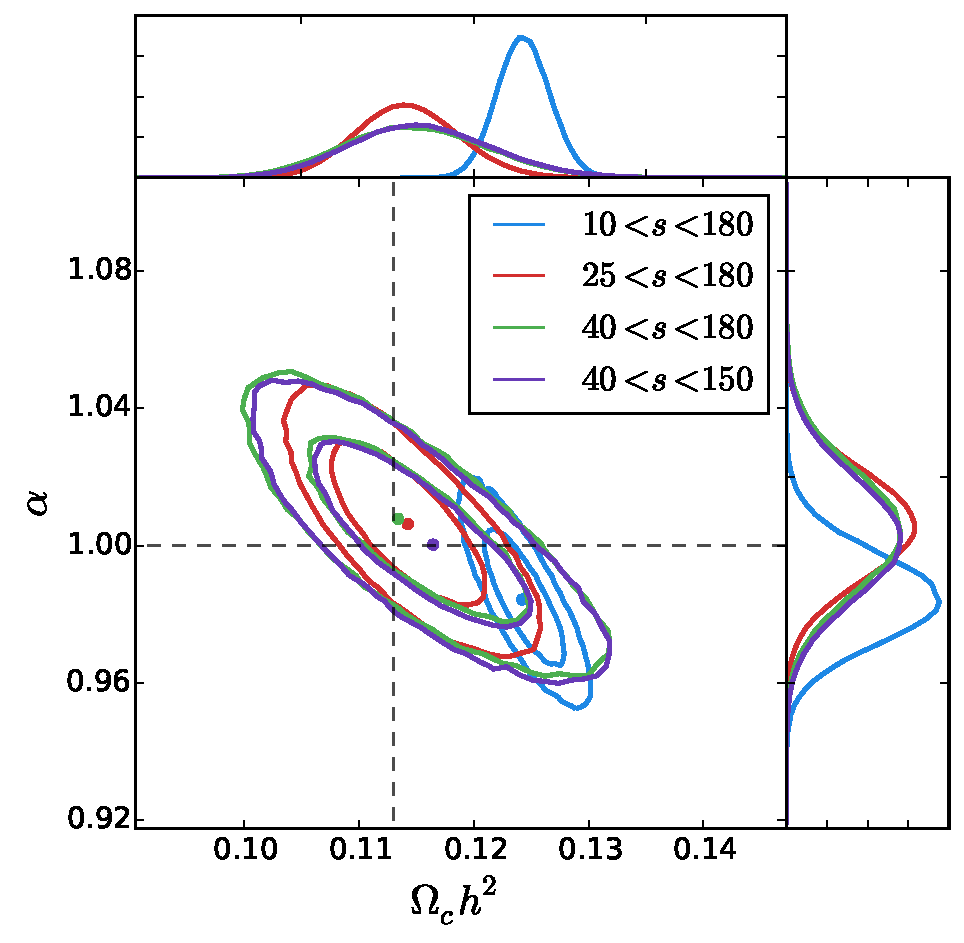
\includegraphics[width=\columnwidth]{images/CdatasetTrunc.pdf}
	\end{center}
	\caption{Four different dataset truncation values are used in fitting to the WizCOLA $z=0.6$ mean dataset. Utilising the $10<s<180 h^{-1}$ Mpc range employed by \citet{BlakeDavis2011} provided strong constraints on the parameters $\Omega_c h^2$ and $\alpha$, but recovered values more than $3-\sigma$ away from the desired outcomes (away from the known parameters used to create the simulation). Increasing the lower bound of the data shifted the recovered parameters to be well below $1-\sigma$ deviation from the desired outcome, at the cost of larger uncertainty in the likelihood surfaces. A reduced upper bound was tested as well due to its presence in prior literature, however minimal impact was found by reducing the upper limit.}
	\label{fig:CdatasetTrunc}
	%\end{wrapfigure}
\end{figure}







\end{document}

